\documentclass[11pt, a4paper, twoside]{Thesis}
\usepackage{etex}
%\usepackage{arabtex}
%\usepackage{utf8}
\usepackage{array}
\usepackage{float}
\usepackage{subcaption}
\usepackage{amsmath}
\usepackage{tocbibind}
%\usepackage{packages/algorithm2e}
\usepackage{multirow}
\usepackage{setspace}
\usepackage{tikz}
\usetikzlibrary{shapes.geometric, arrows}
\usepackage{microtype}
\usepackage{standalone}
\usepackage{tabularx}
\usepackage{booktabs}
% \usepackage{graphicx}
\usepackage[normalem]{ulem}
\useunder{\uline}{\ul}{}
%\usepackage{tabularx}
\usepackage{graphicx}
\usepackage{titlesec}
\graphicspath{ {figures/} }

\usepackage[ruled,vlined,linesnumbered]{algorithm2e}

\newcolumntype{Y}{>{\centering\arraybackslash}X}
\newcolumntype{L}{>{\centering\arraybackslash}m{3cm}}
\setlength{\parindent}{0.7cm}

\makeatletter
\DeclareRobustCommand\onedot{\futurelet\@let@token\@onedot}
\def\@onedot{\ifx\@let@token.\else.\null\fi\xspace}

\titleformat{\paragraph}
{\normalfont\normalsize\bfseries}{\theparagraph}{1em}{}
\titlespacing*{\paragraph}
{0pt}{3.25ex plus 1ex minus .2ex}{1.5ex plus .2ex}

\def\eg{\emph{e.g}\onedot} \def\Eg{\emph{E.g}\onedot}
\def\ie{\emph{i.e}\onedot} \def\Ie{\emph{I.e}\onedot}
\def\cf{\emph{c.f}\onedot} \def\Cf{\emph{C.f}\onedot}
\def\etc{\emph{etc}\onedot} \def\vs{\emph{vs}\onedot}
\def\wrt{w.r.t\onedot} \def\dof{d.o.f\onedot}
\def\etal{\emph{et al}\onedot}
\usepackage[group-separator={,}]{siunitx}

\makeatother

\newcommand{\argmax}{\operatornamewithlimits{argmax}}
\newcommand{\argmin}{\operatornamewithlimits{argmin}}
\newcommand{\abs}[1]{\left\lvert#1\right\rvert}
\newcommand{\norm}[1]{\left\lVert#1\right\rVert}
\newcommand{\listofalgorithmes}{\tocfile{\listalgorithmcfname}{loa}}
\newcommand\Chapter[2]{
  \chapter[#1: {\itshape#2}]{#1\\[1ex]\Large#2}
}

	\begin{document}
\newcommand{\calcic}{\calc^{\subseteq}}

\newcommand{\ICs}{\mathcal{C}}
\newcommand{\Cl}{\mathit{Cl}}

\newtheorem{dtheorem}[theorem]{Theorem}
\newcommand{\NP}{\mathsf{NP}}
\newcommand{\NLOG}{\mathsf{NLogSpace}}
\newcommand{\LOG}{\mathsf{LogSpace}}
\newcommand{\ACzero}{\mathsf{AC}^0}

\newcommand{\leanparagraph}[1]{\smallskip\noindent\textbf{#1}. }

\newcommand{\nop}[1]{}

\newcommand{\calc}{\mathcal{K}_{\mathit{taut}}}

\newcommand{\dlf}[1]{\mathcal{#1}}
\def\rel#1{\mbox{\small\textsc{#1}}}
\def\conc#1{\mbox{\textsf{#1}}}
\def\inst#1{\mbox{\small{\texttt{#1}}}}
\def\axiom#1{\mbox{\textit{#1}}}
\def\var#1{\mbox{\textsl{#1}}}
\def\code#1{\mbox{\small{\texttt{#1}}}}
\def\lex#1{\mbox{{\small``\textsf{#1}''}}}

\makeatletter
\providecommand{\leftsquigarrow}{%
  \mathrel{\mathpalette\reflect@squig\relax}%
}
\newcommand{\reflect@squig}[2]{%
  \reflectbox{$\m@th#1\rightsquigarrow$}%
}
\makeatother

\def\impliedBy{\leftarrow}
\def\la{\leftarrow}
\def\slot{\rightarrow\hspace{-1.3ex}\rightarrow}
\def\tslot{\Rightarrow\hspace{-1.3ex}\Rightarrow}

\newcommand{\dlpluslog}{\ensuremath{\mathcal{DL}\text{+}\mathit{log}}}


\newcommand{\redx}{\ensuremath{\lp^M_x}\xspace}
\newcommand{\redinter}{\ensuremath{\lp^M_\inter}\xspace}

\newcommand{\flpfred}[2]{\ensuremath{{#1^{#2}_{\mathit{f}}}}\xspace}
\newcommand{\flpnred}[2]{\ensuremath{{#1^{#2}_{\mathit{t}}}}\xspace}
\newcommand{\flpcred}[2]{\ensuremath{{#1^{#2}_{\mathit{c}}}}\xspace}
\newcommand{\flpredas}[2]{\ensuremath{{#1^{#2}_{\mathit{FLP}}}}\xspace}
\newcommand{\flpreddllp}[3]{\ensuremath{{#1^{#2,#3}_{\mathit{FLP}}}}\xspace}
\newcommand{\glredas}[2]{\ensuremath{{#1^{#2}_{\mathit{GL}}}}\xspace}
\newcommand{\dlpred}[2]{\ensuremath{{#1^{#2}_{\mathit{d}}}}\xspace}
\newcommand{\strred}[2]{\ensuremath{{#1^{#2}_{\mathit{s}}}}\xspace}
\newcommand{\conf}[1]{\ensuremath{{\mathit{conf}(#1)}}\xspace}

\newcommand{\atom}[2]{\ensuremath{\mathit{#1}(#2)}\xspace}
\newcommand{\ew}[2]{\ensuremath{\mathbf{EW}(\mathit{#1},{#2})}\xspace}
\newcommand{\dlpropatom}[2]{\ensuremath{{
\mathrm{DL}[#1;\,#2]
}}\xspace}

\newcommand{\dlatom}[3]{\ensuremath{{
\dlpropatom{#1}{#2}(#3)
}}\xspace}
%\newcommand{\h}[1]{\ensuremath{\mi{Head()}}}
\newcommand{\ddlatom}[5]{\ensuremath{
\begin{array}{@{}r@{}l@{}}
\mathrm{DL}[#1,& #2 \\
               & #3;\, #4](#5)
\end{array}
}\xspace}

\newcommand{\redfot}{\ensuremath{\lp^M_\fot}\xspace}

\newcommand{\mop}{\ensuremath{\mathsf{L}}\xspace}
\newcommand{\mopb}{\ensuremath{\mathsf{B}}\xspace}
\newcommand{\mopm}{\ensuremath{\mathsf{M}}\xspace}
\newcommand{\mopo}{\ensuremath{\mathsf{O}}\xspace}

\newcommand{\limpl}{\ensuremath{\supset}}
\newcommand{\dnot}{\ensuremath{not\text{ }}}
\newcommand{\snot}{\ensuremath{\sim}\xspace}

\newcommand{\domain}{\ensuremath{U}\xspace}
\newcommand{\sinter}{\ensuremath{\mathbf{I}}\xspace}
\newcommand{\minter}{\ensuremath{\langle \inter, \sinter \rangle}\xspace}
\newcommand{\hinter}{\ensuremath{I}\xspace}
\newcommand{\inter}{\ensuremath{\mathcal{I}}\xspace}
\newcommand{\interfunsym}{\ensuremath{\inter}\xspace}
\newcommand{\interfun}{\ensuremath{\cdot^\interfunsym}\xspace}
\newcommand{\interdef}{\ensuremath{\inter = \langle \domain, \interfun
  \rangle}\xspace}

\newcommand{\logic}{\ensuremath{\mathscr{L}}\xspace}
\newcommand{\lang}{\ensuremath{\mathcal{L}}\xspace}
\newcommand{\flang}{\ensuremath{\mathcal{L}}\xspace}

\newcommand{\fsymb}{\ensuremath{\mathcal{F}}\xspace}
\newcommand{\psymb}{\ensuremath{\mathcal{P}}\xspace}
\newcommand{\psymbc}{\ensuremath{\mathcal{P}_\mathit{c}}\xspace}
\newcommand{\psymbr}{\ensuremath{\mathcal{P}_\mathit{r}}\xspace}
\newcommand{\psymbdl}{\ensuremath{\mathcal{P}_\mathit{o}}\xspace}
\newcommand{\psymblp}{\ensuremath{\mathcal{P}_\mathit{p}}\xspace}
\newcommand{\psymblpi}{\psymblp^{({-})}}
\newcommand{\csymb}{\ensuremath{\mathcal{C}}\xspace}
\newcommand{\vsymb}{\ensuremath{\mathcal{V}}\xspace}

\newcommand{\signature}{\ensuremath{\Sigma}\xspace}
\newcommand{\signaturelp}{\ensuremath{\Sigma_\mathit{p}}\xspace}
\newcommand{\signaturedl}{\ensuremath{\Sigma_\mathit{o}}\xspace}


\newcommand{\dlpsigdef}{\ensuremath{\signature=\langle \fsymb,\psymbdl,\psymblp\rangle}\xspace}
\newcommand{\sigdefdl}{\ensuremath{\signaturedl=\langle \fsymb,\psymbdl\rangle}\xspace}
\newcommand{\sigdeflp}{\ensuremath{\signaturelp=\langle \fsymb,\psymblp\rangle}\xspace}


\newcommand{\hu}{\ensuremath{\mathrm{HU}}\xspace}
\newcommand{\hb}{\ensuremath{\mathrm{HB}}\xspace}


\newcommand\hex{{\sc hex}}
\newcommand{\head}[1]{\ensuremath{H(#1)}\xspace}
\newcommand{\body}[1]{\ensuremath{B(#1)}\xspace}
\newcommand{\pbody}[1]{\ensuremath{B(#1)^+}\xspace}
\newcommand{\nbody}[1]{\ensuremath{B(#1)^-}\xspace}

\newcommand{\HBi}[3]{\ensuremath{\hb_{#1,#2}(#3)}\xspace}
\newcommand{\HBis}[3]{\ensuremath{\hb_{#1,#2}^*(#3)}\xspace}
\newcommand{\HB}[1]{\ensuremath{\hb(#1)}\xspace}
\newcommand{\HU}[1]{\ensuremath{\hu(#1)}\xspace}

\newcommand{\DLA}[1]{\ensuremath{\mathrm{D({#1})}}\xspace}
\newcommand{\DLAq}{\ensuremath{\mathrm{DL}^{?}}\xspace}
\newcommand{\DLAp}{\ensuremath{\mathrm{DL}^{+}}\xspace}

\newcommand{\DLApm}{\ensuremath{\mathrm{DL}_{m}^{+}}\xspace}
\newcommand{\DLApa}{\ensuremath{\mathrm{DL}_{a}^{+}}\xspace}
\newcommand{\DLAqm}{\ensuremath{\mathrm{DL}_{m}^{?}}\xspace}
\newcommand{\DLAqa}{\ensuremath{\mathrm{DL}_{a}^{?}}\xspace}

\newcommand{\DLAm}{\ensuremath{\mathrm{DL}}\xspace}


\newcommand{\hm}{\ensuremath{HM}\xspace}

\newcommand{\gr}[1]{\ensuremath{gr(#1)}\xspace}
\newcommand{\grset}[2]{\ensuremath{gr_{#2}(#1)}\xspace}
\newcommand{\gro}[1]{\ensuremath{gr_o(#1)}\xspace}

\newcommand{\AS}[1]{\ensuremath{\mathrm{AS}(#1)}\xspace}
\newcommand{\cAS}[1]{\ensuremath{\mathrm{AS^c}(#1)}\xspace}
\newcommand{\fAS}[1]{\ensuremath{\mathrm{AS^f}(#1)}\xspace}
\newcommand{\nAS}[1]{\ensuremath{\mathrm{AS^t}(#1)}\xspace}

\newcommand{\lp}{\ensuremath{\Pi}\xspace}
\newcommand{\DL}{\fot}
\newcommand{\fot}{\ensuremath{\cO}\xspace}

\newcommand{\modl}{\ensuremath{\lang_{\mop}}\xspace}
\newcommand{\fmodl}{\ensuremath{\flang_{\mop}}\xspace}
\newcommand{\fmodlcomb}{\ensuremath{\flang_{\mop}^{\flang \cup \lp}\xspace}}
\newcommand{\fmodlnoq}{\ensuremath{\fmodl'}\xspace}

\newcommand{\varsub}{\ensuremath{\beta}\xspace}
\newcommand{\varass}{\ensuremath{B}\xspace}

\newcommand{\shoiqd}{\ensuremath{\mathcal{SHOIQ}(\mathbf{D})}\xspace}
\newcommand{\dlr}{\ensuremath{\mathcal{DLR}}\xspace}
\newcommand{\dlrom}{\ensuremath{\mathcal{DLRO}^{-\{\leq\}}}}
\newcommand{\dlro}{\ensuremath{\mathcal{DLRO}}}
\newcommand{\shoind}{\ensuremath{\mathcal{SHOIN}(\mathbf{D})}\xspace}
\newcommand{\shoiq}{\ensuremath{\mathcal{SHOIQ}}\xspace}
\newcommand{\shoq}{\ensuremath{\mathcal{SHOQ}}\xspace}
\newcommand{\sroiq}{\ensuremath{\mathcal{SROIQ}}\xspace}
\newcommand{\shif}{\ensuremath{\mathcal{SHIF}}\xspace}
\newcommand{\shifd}{\ensuremath{\mathcal{SHIF}(\mathbf{D})}\xspace}
\newcommand{\shiq}{\ensuremath{\mathcal{SHIQ}}\xspace}
\newcommand{\shiqd}{\ensuremath{\mathcal{SHIQ}(\mathbf{D})}\xspace}
\newcommand{\shoin}{\ensuremath{\mathcal{SHOIN}}\xspace}
\newcommand{\alc}{\ensuremath{\mathcal{ALC}}\xspace}
\newcommand{\alchiq}{\ensuremath{\mathcal{ALCHIQ}}\xspace}
\newcommand{\alcnr}{\ensuremath{\mathcal{ALCNR}}\xspace}
\newcommand{\elpp}{\ensuremath{\mathcal{EL}^{++}}\xspace}
\newcommand{\dllite}{\ensuremath{\mathit{DL\text{-}Lite}}\xspace}


\newcommand{\datalog}{\textsc{Datalog}\xspace}
\newcommand{\datalogv}{$\mbox{\textsc{Datalog}}^{\lor}$\xspace}
\newcommand{\datalogn}{$\mbox{\textsc{Datalog}}^{\neg}$\xspace}
\newcommand{\datalogvn}{$\mbox{\textsc{Datalog}}^{\lor,\neg}$\xspace}

%\newcommand{\wrt}{w.r.t.\xspace}
%\newcommand{\ie}{i.e.,\xspace}
%\newcommand{\eg}{e.g.,\xspace}
%\newcommand{\vs}{vs.\xspace}

\newcommand{\dllog}{$\dlf{DL}$\mbox{+}\textsc{log}\xspace}
\newcommand{\comblog}[1]{$\dlf{#1}$\mbox{+}\textsc{log}\xspace}



\newcommand{\dlvhex}{DLVHEX\xspace}

%% COMPLEXITY CLASSES



\newcommand{\logspace}{\textsc{LogSpace}\xspace}

\newcommand{\nlogspace}{\textsc{NLogSpace}\xspace}

\newcommand{\ptime}{\textsc{PTime}\xspace}

\newcommand{\p}{\textsc{P}\xspace}
\newcommand{\pc}{\textsc{P}\complete\xspace}

\newcommand{\ph}{\textsc{PH}\xspace}

\newcommand{\np}{\textsc{NP}\xspace}
\newcommand{\complete}{\text{-complete}}
\newcommand{\completeness}{\text{-completeness}}
\newcommand{\npc}{\textsc{NP}\complete\xspace}

\newcommand{\conp}{\textsc{co-NP}\xspace}
\newcommand{\conpc}{\textsc{co-NP}\complete\xspace}

\newcommand{\pip}[1]{\ensuremath{\Pi^P_{#1}}\xspace}
\newcommand{\sigmap}[1]{\ensuremath{\Sigma^P_{#1}}\xspace}
\newcommand{\deltap}[1]{\ensuremath{\Delta^P_{#1}}\xspace}

\newcommand{\transflpsem}[1]{\ensuremath{\rho({#1})}\xspace}
\newcommand{\transposdlsimnormal}[1]{\ensuremath{\nu({#1})}\xspace}


\newcommand{\pspace}{\textsc{PSpace}\xspace}

\newcommand{\psp}{\pspace}

\newcommand{\exptime}{\textsc{ExpTime}\xspace}
\newcommand{\exptimec}{\textsc{ExpTime}\complete\xspace}
\newcommand{\exptimecs}{\textsc{ExpTime}\completeness\xspace}

%\newcommand{\C}{\textsc{C}\xspace}
\newcommand{\nexptime}{\textsc{NExpTime}\xspace}
\newcommand{\nexptimec}{\textsc{NExpTime}\complete\xspace}
\newcommand{\nexptimecs}{\textsc{NExpTime}\completeness\xspace}
\newcommand{\nexp}{\textsc{NExp}\xspace}
\newcommand{\nexpc}{\textsc{NExp}\complete\xspace}

\newcommand{\conexptime}{\textsc{co-NExpTime}\xspace}
\newcommand{\conexp}{\textsc{co-NExp}\xspace}
\newcommand{\conexpc}{\textsc{co-NExp}\complete\xspace}

\newcommand{\exptimen}[1]{\textsc{{#1}ExpTime}\xspace}

\newcommand{\nnexptime}[1]{\textsc{{#1}NExpTime}\xspace}


\newcommand{\nconexptime}[1]{\textsc{co-{#1}NExpTime}\xspace}

\newcommand{\nexptimeNP}{\ensuremath{\textsc{NExpTime}^\textsc{NP}}\xspace}



\newcommand{\ckb}{\ensuremath{\mathcal{KB}}\xspace}



\newcommand{\ckbdef}{\ensuremath{\mathcal{KB} = \langle \fot, \lp
    \rangle}\xspace}

\newcommand{\citeN}[1]{\protect\citeauthor{#1}~\shortcite{#1}\protect}


\newcommand{\dlextension}[2]{\ensuremath{\tau^{#1}(#2)}}

% queries
% certain answers
\newcommand{\cansw}[2]{\ensuremath{\mathit{cansw}(#1,#2)}}
% skeptical answers
\newcommand{\pansw}[2]{\ensuremath{\mathit{pansw}(#1,#2)}}

\newcommand{\st}{\ensuremath{\,.\,}}
\newcommand{\names}{\ensuremath{\mathcal{N}}\xspace}

% DL-program
%\newcommand{\dlpdef}{\ensuremath{\dlp=(\DL,\lp)}\xspace}
\newcommand{\dlpdef}{\ensuremath{P=(\DL,\lp)}\xspace}
\newcommand{\dlp}{\ensuremath{\mathcal{KB}}\xspace}

\newcommand{\dlpi}[2]{\ensuremath{\mathcal{KB}_{#1,#2}}\xspace}
\newcommand{\dlpis}[2]{\ensuremath{\mathcal{KB}_{#1,#2}^*}\xspace}

\newcommand{\lpis}[2]{\ensuremath{\lp_{#1,#2}^*}\xspace}
\newcommand{\tuple}[1]{\langle#1\rangle}
\newcommand{\cA}{\mathcal{A}}
\newcommand{\cC}{\mathcal{C}}
\newcommand{\cG}{\mathcal{G}}
\newcommand{\cO}{\mathcal{O}}
\newcommand{\cP}{\mathcal{P}}
\newcommand{\cT}{\mathcal{T}}
\newcommand{\cS}{\mathcal{S}}
\newcommand{\cN}{\mathcal{N}}
\newcommand{\cH}{\mathcal{H}}
\newcommand{\cU}{\mathcal{U}}
\newcommand{\bR}{\mathbf{R}}
\newcommand{\bC}{\mathbf{C}}
\newcommand{\bI}{\mathbf{I}}
\newcommand{\bS}{\mathbf{S}}
\newcommand{\bP}{\mathbf{P}}
\newcommand{\cR}{\mathcal{R}}
\newcommand{\myequation}[4]{%
\newcommand{\h}
\vspace*{#1\baselineskip}

\begin{equation}
\label{#2}
#3
\end{equation}

\vspace*{#4\baselineskip}
}


\newcommand{\FLP}{\ensuremath{\mathit{flp}}\xspace}

\newcommand{\mi}[1]{\mathit{#1}}
\newcommand{\Supp}{\mi{Supp}}

\newcommand{\NewRAnsSet}{\ensuremath{\mathit{SupRAnsSet}}}


\newcounter{myenumctr}
\newenvironment{myenumerate}{\begin{list}{(\arabic{myenumctr})}{\usecounter{myenumctr}
\topsep=0pt
\setlength{\leftmargin}{0.5\labelwidth}
\setlength{\itemindent}{1.5\labelwidth}
\setlength{\itemsep}{0cm}}}
{\end{list}}



% definition of uminus operator sign

\def\uminus{\setbox0=\hbox{$\cup$}\rlap{\hbox
    to\wd0{\hss\raise0.3ex\hbox{$\scriptscriptstyle{-}$}\hss}}\box0}

\def\uminusstar{\setbox0=\hbox{$\cup$}\rlap{\hbox
    to\wd0{\hss\raise0.3ex\hbox{$\scriptscriptstyle{-^\star}}\hss}}\box0}


% definition of alternative uplus operator sign

\def\myuplus{\setbox0=\hbox{$\cup$}\rlap{\hbox
    to\wd0{\hss\raise0.4ex\hbox{$\scriptscriptstyle{+}$}\hss}}\box0}


% definition of capminus operator sign

\def\cminus{\setbox0=\hbox{$\cap$}\rlap{\hbox
    to\wd0{\hss\raise0.3ex\hbox{$\scriptscriptstyle{-}$}\hss}}\box0}


\def\cminusstar{\setbox0=\hbox{$\cap$}\rlap{\hbox
    to\wd0{\hss\raise0.3ex\hbox{$\scriptscriptstyle{-}$}\hss}}\box0^\star}

\newcommand{\lpor}{\mid}

\newcommand{\naf}[1]{\ensuremath{\mathit{not}~ #1}}

\newcommand{\uplusc}{\ensuremath{\uplus_c}}
\newcommand{\uminusc}{\ensuremath{\uminus_c}}
\newcommand{\cminusc}{\ensuremath{\cminus_c}}

\newcommand{\uplusi}{\ensuremath{\uplus_i}}
\newcommand{\uminusi}{\ensuremath{\uminus_i}}
\newcommand{\cminusi}{\ensuremath{\cminus_i}}

\newcommand{\upluso}{\ensuremath{\uplus_\mathrm{opt}}}
\newcommand{\uminuso}{\ensuremath{\uminus_\mathrm{opt}}}
\newcommand{\cminuso}{\ensuremath{\cminus_\mathrm{opt}}}
% A single rule outside a program.
\newcommand{\prule}[2]{\ensuremath{\mathit{#1}\gets\mathit{#2}}}

% stable model of a Combined KB:
%\newcommand{\smodels}{\ensuremath{\models_s}}

% for logic programs
\newenvironment{program}{\[\begin{array}{rll}}{\end{array}\]}
\newcommand{\tsrule}[2]{\ensuremath{\mathit{#1} &\gets& \mathit{#2}\\}}


\newcommand{\mknflang}{\ensuremath{\lang_{\mathit{MKNF}}}\xspace}
\newcommand{\mknfmodels}{\ensuremath{\models^{\mopk,\mopnot}}\xspace}
\newcommand{\ssmodels}{\ensuremath{\models_{S5}}\xspace}

\newcommand{\amodels}{\ensuremath{\models_{\mathit{a}}}\xspace}
\newcommand{\cmodels}{\ensuremath{\models_{\mathit{c}}}\xspace}
\newcommand{\fmodels}{\ensuremath{\models_{\mathit{f}}}\xspace}
\newcommand{\nmodels}{\ensuremath{\models_{\mathit{t}}}\xspace}


\newcommand{\mknfinter}{\ensuremath{M}\xspace}
\newcommand{\mknfstructure}{\ensuremath{(\inter, \mknfinter, N)}\xspace}


\newcommand{\mopk}{\ensuremath{\mathsf{K}}\xspace}
\newcommand{\mopnot}{\ensuremath{\mathsf{not}}\,}

% more compact itemize environments
\newenvironment{myitemize}
   {\begin{itemize}\setlength{\itemsep}{-0.08cm}}{\end{itemize}}


\newcommand{\be}{\begin{enumerate}}
\newcommand{\ee}{\end{enumerate}}

\newcommand{\shoinSWRL}{\shoin-SWRL\xspace}

\newcommand{\smallfol}{{\text{\footnotesize{+FOL}}}}
\newcommand{\smalldl}{{\text{\footnotesize{+DL}}}}
\newcommand{\folflogic}{$\text{F}^{\smallfol}\text{-Logic}$\xspace}
\newcommand{\dlflogic}{$\text{F}^{\smalldl}\text{-Logic}$\xspace}
\newcommand{\folfmodels}[1]{\ensuremath{{\ \models_{\mathsf{f},#1}\ }}\xspace}
\newcommand{\nfolfmodels}[1]{\ensuremath{{\ \nmodels_{\mathsf{f},#1}\ }}\xspace}

%\newcommand{\DLmodels}{\ensuremath{{\ \models_\DL\ }}\xspace}
\newcommand{\cdlmodels}{\ensuremath{{\ \models_{\DL,c}\ }}\xspace}

% combined signature
\newcommand{\csig}{\ensuremath{\langle \signature_\Phi, \signature_P \rangle}\xspace}

\newcommand{\attr}[1]{\ensuremath{\twoheadrightarrow\!\!#1}\xspace}
\newcommand{\type}[1]{\ensuremath{:\!\!#1}\xspace}
\def\bD{\mathbf{D}}
\newcommand{\cE}{{\mathbf E}}
\newcommand{\cV}{\mathcal{V}}



\def\DLB{{\it L}}
\newcommand{\bt}{\begin{tabular}}
\def\cI{{\cal I}}


\newcommand{\et}{\end{tabular}}
\newcommand{\bs}{\begin{theorem}}
\newcommand{\es}{\end{theorem}}
\newcommand{\bsw}[1]{\begin{theorem}[#1]}
\newcommand{\esw}{\end{theorem}}
\newcommand{\bc}{\begin{corollary}}
\newcommand{\ec}{\end{corollary}}
\newcommand{\bcw}[1]{\begin{corollary}[#1]}
\newcommand{\ecw}{\end{corollary}}
\newcommand{\ble}{\begin{lemma}}
\newcommand{\ele}{\end{lemma}}
\newcommand{\blew}[1]{\begin{lemma}[#1]}
\newcommand{\elew}{\end{lemma}}
\newcommand{\bp}{\begin{proposition}}
\newcommand{\ep}{\end{proposition}}
\newcommand{\bd}{\begin{definition}\rm}
\newcommand{\ed}{\end{definition}}
\newcommand{\bdw}[1]{\begin{definition}[#1]\rm}
\newcommand{\edw}{\end{definition}}
\newcommand{\ba}{\begin{algorithm}\rm}
\newcommand{\ea}{\end{algorithm}}
\newcommand{\baw}[1]{\begin{algorithm}[#1]\rm}
\newcommand{\eaw}{\end{algorithm}}
\newcommand{\bbs}{\begin{example}\rm}
\newcommand{\ebs}{\end{example}}
\newcommand{\bbsw}[1]{\begin{example}[#1]\rm}
\newcommand{\ebsw}{\end{example}}
\newcommand{\bb}{\begin{remark}\rm}
\newcommand{\eb}{\end{remark}}
\newcommand{\beq}{\begin{eqnarray*}}
\newcommand{\eeq}{\end{eqnarray*}}
\newcommand{\baq}{\begin{array}}
\newcommand{\eaq}{\end{array}}


\newcommand{\mids}{\,{\mid}\,}
\newcommand{\ins}{\,{\in}\,}
\newcommand{\gts}{\,{>}\,}
\newcommand{\ges}{\,{\ge}\,}
\newcommand{\les}{\,{\le}\,}
\newcommand{\lts}{\,{<}\,}
\newcommand{\eqs}{\,{=}\,}
\newcommand{\eq}{\ensuremath{\eqs\!}}
\newcommand{\diff}{\ensuremath{\neqs\!}}
\newcommand{\neqs}{\,{\neq}\,}
\newcommand{\modelss}{\,{\models}\,}
\newcommand{\notmodelss}{\,{\not\models}\,}
\newcommand{\cups}{\,{\cup}\,}
\newcommand{\caps}{\,{\cap}\,}
\newcommand{\subseteqs}{\,{\subseteq}\,}
\newcommand{\sqsubseteqs}{\,{\sqsubseteq}\,}

%\ifdraft
%\newcommand{\comment}[1]{{\textcolor{blue}{*** #1 ***}}}
%\else
%\newcommand{\comment}[1]{}
%\fi

\newcommand{\missing}[1]{{\textcolor{red}{* #1?*}}}


%\setcode{utf8}

% *************** Front matter ***************
\frontmatter

\title  {Immotion - Exergame for Warm Up Guidance and Motivation}

\authors  {\texorpdfstring
            {{Marko Vuji\'c}}
            {}
            }
\addresses  {\groupname\\\deptname\\\univname}  % Do not change this here, instead these must be set in the "Thesis.cls" file, please look through it instead
%\usdate
\date       {Saarbr\"ucken, \today }
\subject    {}
\keywords   {}

\maketitle

%\newpage
%\mbox{}
%\thispagestyle{empty}
%\newpage

\setstretch{1.3}

\thispagestyle{empty}
\setcounter{tocdepth}{5}
\section*{Eidesstattliche Erkl\"{a}rung}
Ich erkl\"{a}re hiermit an Eides Statt, dass ich die vorliegende Arbeit selbstst\"{a}ndig verfasst und keine
anderen als die angegebenen Quellen und Hilfsmittel verwendet habe.

\vspace{0.60cm}
\section*{Statement in Lieu of an Oath}
I hereby confirm that I have written this thesis on my own and that I have not used any other media or
materials than the ones referred to in this thesis.
\vspace{1.5cm}

\section*{Einverst\"{a}ndniserkl\"{a}rung}
Ich bin damit einverstanden, dass meine (bestandene) Arbeit in beiden Versionen in die Bibliothek der
Informatik aufgenommen und damit ver\"{o}ffentlicht wird.

\vspace{0.60cm}
\section*{Declaration of Consent}
I agree to make both versions of my thesis (with a passing grade) accessible to the public by having
them added to the library of the Computer Science Department.
\vspace{3cm}

\begin{flushright}
\noindent Saarbr\"{u}cken, \today
\hfill
Marko Vuji\'c
\end{flushright}

\clearpage  % Declaration ended, now start a new page
%% ----------------------------------------------------------------

%%\newpage
%\mbox{}
%\thispagestyle{empty}
%\newpage

% The Abstract Page
\addtotoc{Abstract}  % Add the "Abstract" page entry to the Contents
\abstract{Past research related to exergames has found that they can help to motivate people to exercise by converting physical activity into an enjoyable game. However, these exergames have been single purpose usually home fitness only. In this thesis, we designed an exergame for warm up guidance and motivation to be used in gyms and fitness centers before physically more strenuous exercise. We utilized immersive technologies based on the hypothesis that they can be used as a guiding tool for warm up procedures, would increase warm up duration, and increase exercise enjoyment. By making the game interactive and appealing, with intervals that last as long as the player chooses to, the warm up procedure undergoes a shift from a repetitive and tiresome activity to an entertaining and challenging necessity. In order to evaluate our exergame, we conducted a user study comparing warm up procedure with a video showing a fitness instructor performing a warm up session to a warm up procedure with our exergame. In both conditions, the movements the participants needed to perform were identical. The usage of the exergame, showed a statistically significant increase in exercise duration relative to the non-gaming condition. TODO% The exergame showed a significant increase in user motivation and enjoyment when compared to the non gaming condition, with the Kinect condition found to be slightly more motivating than the screen condition.
\addtocontents{toc}{\vspace{1em}}  % Add a gap in the Contents, for aesthetics
%The current study employed an in-house developed exergame and manipulated the game features in a 2 (autonomy-supportive game features: on vs. off) × 2 (competence-supportive game features: on vs. off) experiment to predict need satisfaction, game enjoyment, motivation for future play, effort for gameplay, self-efficacy for exercise using the game, likelihood of game recommendation, and game rating.
\clearpage

%% ----------------------------------------------------------------
%\newpage
%\mbox{}
%\thispagestyle{empty}
%\newpage

\setstretch{1.3}  % Reset the line-spacing to 1.3 for body text (if it has changed)

% The Acknowledgements page, for thanking everyone
\acknowledgements{
\addtocontents{toc}{}  % Add a gap in the Contents, for aesthetics    \vspace{1em}


}
\clearpage  % End of the Acknowledgements
%% ----------------------------------------------------------------
%\newpage
%\mbox{}
%\thispagestyle{empty}
%\newpage

%\newpage
%%\mbox{}
\thispagestyle{empty}
%\newpage

\setstretch{1}
\begin{spacing}{0.1}
\pagestyle{fancy}
\tableofcontents
%\newpage
\listoffigures	
%\newpage
\listoftables
%\newpage
%\listofalgorithmes
\end{spacing}

\clearpage

\setstretch{1.3}
% *************** Main matter ***************
\mainmatter

%\chapter{Introduction}
\label{chap:intro}

\section{Motivation}
\label{chap:motivation}

%\chapter{Literature review}\label{chapter:warmup}
%Deterding et al. go on to explain that a gamified system, like a game, usually has rules and is goal oriented. Gamification is not a full-fledged game, although it utilizes many techniques that games implement such as, levels, clear goals, time constraints, badges, value conscious game design, challenge, limited resources and leader boards. It allows people to stay grounded in reality, whilestill profiting from successful game benefits like gaining access to a person’s emotions and intrinsic motivation, which in turn will help create habits. ZA ABRSTACT??
The following chapter provides an overview of the past research related to warm up (WU) as a preparatory exercise prior to performing physical activity, theories that describe and explain user's engagement and motivation when interacting with a gamified system and conceptually related works in the domain of gamified solutions relevant to fitness and exercise. In other words, this section explores the overlap of five different fields, namely exergames and gamification, health and fitness, injury prevention and motivational psychology. This concept is illustrated in Figure \ref{fig:diagram}.
\begin{figure}[h]
    \centering
    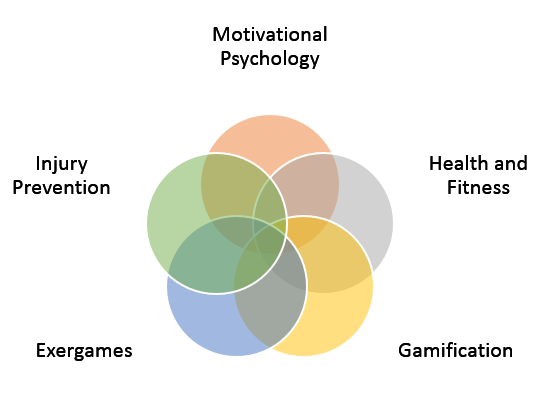
\includegraphics[width=0.75\textwidth]{diagram}
    \caption{The five general fields that relate to this work. The target field is presented as the overlap of the five fields}
    \label{fig:diagram}
\end{figure}
To impose structure, first the basic concepts related to warm up and an overview of studies and results regarding the benefits of WU is given. Following, the concepts of gamification and exergames are introduced. Finally, a comparison between the presented approaches and our solution will be made together with the direction the
research in this thesis will take, and the motivations behind it.
\section{Warm Up in Sports}
\subsection{The Importance of Physical Activity}
In the last few decades, there has been a significant increase of women and men who engage in some sort of physical activity. Physical activity is beneficial to ones health. According to medical professionals, regular physical activity can significantly decrease the commonness of chronic diseases such as high blood pressure, heart disease,
(colon and breast) cancer, hypertension and diabetes as well as reduce cardiovascular-related deaths, to name a few \cite{mayr2015prevention, warburton2006health}. Regular exercise reduces the incidence of obesity
and obesity-related illnesses, maintains a general standard of health, and is associated with a reduced risk of premature death \cite{warburton2006health}. Moreover, regular engagement in sports of any kind can also pose as a countermeasure for psychological disorders and greatly limit the severity of
episodes of anxiety and depression \cite{mayr2015prevention}.
\subsection{Overview of Sports Injury}\label{subsection:injury}
The counterpart to all of the mentioned health benefits is that engaging in regular physical activity is often associated with a higher risk of injury which can occur in athletes of all age \cite{van1997severity}. To put it differently, there exists a higher risk of injury of the musculoskeletal system including soft tissue
damage, fractures, ligament and tendon tears, and nerve injuries in athletes who engage in some sort of physical (sport) activity \cite{mayr2015prevention}. Sport related injuries generally occur in joints: the knee, ankle, hip, shoulder, elbow, wrist and spine, usually from a sports related accident but often due to overuse, repetitive microtraumas that are solely insufficient to cause macroscopic injuries
 \cite{mayr2015prevention}. During international athletics championships between 2007 and 2014, data regarding injuries has been collected in order to compare the characteristics of injuries between female and male athletes \cite{edouard2015sex}. The results showed that males suffered more thigh strains than female athletes and that injury incidences differed between genders for location, type and event groups. The results concerning main injury locations for female and male athletes are presented in figure \ref{fig:injuries}. The type of the injury depends on many factors, and usually is divided into: \textit{intrinsic} and \textit{extrinsic} \cite{mayr2015prevention}. The various types of injuries and their corresponding causes are presented in Appendix A (Figure %\ref{chapter:warmup}
). Generally, extrinsic injuries are linked to the practice of sports itself and the environment the activity is catrried out. On the other hand, intrinsic injuries are tied to biological characteristics, anatomical factors, gender, and age, among others \cite{mayr2015prevention}. Fischer \textit{et al.} (2016) differentiate between \textit{damage} as an overuse injury and \textit{injury} as an acute injury. They further state that an injury occurs in a single acute action (acute injury), while damage appears after repeated action as the result of many repetitive minor insults (overuse injury) \cite{fischer2016causes}. In their book \textit{Overuse Injuries of the Musculoskeletal System}, Pecina and Bojanic (1993) state how ``the main characteristic of an injury is acuteness, whereas damage has a chronic character'' \cite{pecina1993overuse}. Acute injuries are more likely to occur in sports that include high-speed running, rapid movement, or full-body contact, whereas aerobic low-contact sports that include long training sessions may produce overuse injuries  \cite{mayr2015prevention}.
\begin{figure}[h]
    \centering
    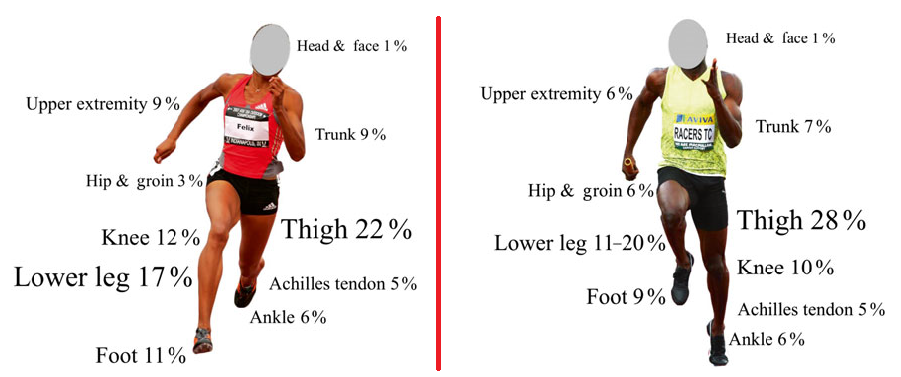
\includegraphics[width=0.85\textwidth]{injuries}
    \caption{Main injury location for female and male athletes during
international athletics championships from 2007 to 2014. Adapted from \cite{mayr2015prevention}}
    \label{fig:injuries}
\end{figure}\\
In order to prevent injuries, athletes should receive the correct amount of training and recovery period, and have a healthy lifestyle. The correct amount of training depends on the type of the physical activity itself, as much as the physical characteristics of the athlete. Moreover, the sports technique must be correct and, in case it is required, a good quality equipment should be used that is adapted to the player (morphology and level of play) in order to prevent injuries. Injury prevention strategies should be gender-specific. That is, as discussed in \cite{edouard2015sex} and presented in Figure \ref{fig:injuries}, for injury prevention ``one size does not fit all'', and hence it should be adapted to the differences in injury characteristics between female and male athletes. Lastly, studies reccomend that every physical activity must be preceded by a suitable warm up procedure which gives athletes time to adjust for a more intense activity, and should end with a cooling down phase \cite{mayr2015prevention}. Next, a definition and an overview of WU prior sport activities is given. %NISI BAS PUNO O WARM UP + INJURY PREVENTION PISAO OVDE  
\subsection{Defining Warm Up}
Despite very contrasting beliefs and limited scientific evidence regarding its effectiveness in many situations, WU has become a standard practice among professional and recreational athletes \cite{bishop2003warm1, bishop2003warm2, shellock1985warming}. WU in sports is defined as a period of preparatory exercise which is carried out in order to prepare the athlete for the demands of the subsequent physical activity  \cite{karvonen1992importance, woods2007warm, hedrick1992exercise}.
%karvonen skini i procitaj
Typically, WU includes a short and low-intensity preparatory activity which is followed by a stretching routine and sports specific exercise \cite{safran1989warm}. 
The ideal WU depends on the physical activity performed,
the level of competition and the age of the participants and should include the muscle groups that are required during the training or competition
 \cite{mayr2015prevention}.Various studies point out that the main purpose of WU is to enhance the subsequent competition or training performance and improve muscle dynamics to reduce the risk of sport-related injury \cite{bishop2003warm1, shellock1985warming, knudson2008warm}. 
 %HERE MENTION THE STUDIES THAT SAY THIS DOESNT HELP.  CHECK LEMON ILIEV
Nonetheless, there is still deficiency of scientific evidence on what kind of WU can influence both muscle damage prevention and performance improvement \cite{safran1989warm}.\\ The following section will shed lights on some of the assumed benefits of WU as a preparatory routine before physically more demanding exercise. 
\subsection{The Benefits of Warm Up}
Fradkin \textit{et al.} (2010) carried out a systematic review and meta-analysis of relevant studies concerning the benefits of WU on performance. They found that an adequate WU supports an improvement in performance in 79\% of the research studies analyzed. Furthermore, they pointed out that there exists little evidence supporting detrimental effects WU might have on performance and sports participants.
WU can affect the performance via variety of temperature and non-temperature related mechanisms \cite{bishop2003warm1}. 
%By performing a low intensity training routine before taking part in more demanding exercise, an increase in one's body temperature \(Magnusson 
%et al., 2000\) and muscle blood flow occurs \(Tiidus \& Shoemaker, 1995\).  
The most relevant effects of WU can be attributed to physiological mechanisms like increased muscle temperature, decreased resistance of muscle and joints (decreased stiffness), increased oxygen delivery to muscles, increased nerve-conduction rate and speeding of metabolic reactions \cite{bishop2003warm1}. 
However, the benefits of WU are not exclusively physical. Apart from the physiological changes a body undergoes during this preparatory period, it has been hypothesized that a possible psychological benefit can also be gained by following a proper WU routine \cite{bishop2003warm1,shellock1985warming}.
It has been suggested that WU can serve as a preparatory phase, providing time for athletes to concentrate and mentally prepare for the forthcoming exercise \cite{shellock1985warming}. 
%Thus, possible psychological benefits is increased mental preparedness for the forthcoming exercise\cite{bishop2003warm1}. 
Moreover, in the study that investigated the link between a WU and psychological processes, Ladvig (2013) reported that athletes who performed a proper WU routine before engaging in more demanding physical activity demonstrated significantly higher levels of exercise related motivation and enjoyment. Thus, increased motivation and enjoyment is an additional psychological benefit of WU \cite{ladwig2013psychological}.
 %findings of this theisis: http://aut.researchgateway.ac.nz/bitstream/handle/10292/325/WeerapongP.pdf?sequence=1
\\Apart from physiological and psychological benefits, WU has been suggested to have an important role in sports-related injury prevention \cite{shellock1985warming}. Unfortunately, there exist no high-quality research studies in order to draw a definite conclusion as to the effect WU has on sports-related injury prevention \cite{fields2007should}. Fradkin \textit{et al.} (2006) reviewed five
high-quality studies that investigated the effects of warming up in humans on injury risk in physical activity \cite{fradkin2006does}. Five studies reported sufficient data on the effects of warming up on reducing injury risk in humans. However, only three of the studies found that performing a WU prior to performance significantly reduced the risk of injury in athletes, while the remaining two found that warming up has no effects in injury decrease\cite{fradkin2006does}. Therefore, the reearchers concluded that there is insufficient evidence to endorse or discontinue WU routine prior to physical activity in order to prevent injury among sports participants. However, the weight of evidence is in favour of a decreased risk of injury \cite{fradkin2006does}. Safran, \textit{et al.} (1989), proposed a possible bio-mechanical explanation for injury reduction with WU. The results of this study showed that warmed-up muscles in the animal models can elongate more before failure caused by increased force and length of stretch \cite{safran1989warm}.\\ According to some studies, an appropriate WU procedure should consist of three factors. These factors represent the WU components mentioned most often in the WU literature: 
\begin{itemize}
\item a period of aerobic exercise to increase body
temperature \cite{safran1989warm},
\item a period of sport-specific stretching to stretch 
the muscles to be used in the subsequent
performance \cite{safran1989warm}, and
\item a period of activity incorporating movements
similar to those to be used in the subsequent
performance \cite{safran1989warm}.
\end{itemize}
%Furthermore, Nosaka and Clarckson found that high and low intensities of WU could reduce the magnitude musculatory damage ... They proposed that 
%A search of the literature identified only one published research paper on the effects of warm-up on the severity of muscle damage (Nosaka & Clarkson, 1997).  Nosaka and Clarkson (1997) found that both high (100 repetitions of maximal concentric contraction) and low (100 repetitions of minimal concentric contraction) intensities of 
%warm-up could reduce the magnitude of mu
%scle damage as indicated by reduced 
%soreness sensation, strength and range of 
%motion loss, swelling, and creatine kinase 
%activity.  The authors proposed that warm-up 
%might help to increase muscle temperature 
%and circulation, and consequen
%tly, increase muscle and conne
%ctive tissue el
%asticity
%the majority of effects of warm up have been attributed to temperature related mechanism
%TO DISCUSS STRETCHING! HERE %
%ne znam da li je ovo za komponenete dobro ovde? mozda bi trebao dodati jos nesto..
\subsection{The Types of Warm Up}
There exist various types of WU procedures that professional and recreational athletes at any level use as a preparatory phase for the more physically demanding exercise. First, it is important to distinguish between WU and stretching activities. While WU mainly focuses on core body temperature elevation, stretching involves movements that stretch the muscle in order to increase the range of motions of joints or group of joints \cite{knudson2008warm}. 
Generally, WU procedures can be classified into \textit{passive} and \textit{active} WU procedures, and are centered on increase in core and muscle temperature. However, they accomplish this objective through different approaches. The former involves raising muscle or core temperature by some external means (e.g. hot showers, saunas), while the latter aims to increase the body temperature through active movements of the major muscle groups (e.g. jogging, cycling, swimming) \cite{shellock1985warming, bishop2003warm2}. The most effective WU that could potentially affect the subsequent performance generally depends on the duration, intensity and the nature of the sports activity to be performed \cite{bishop2003warm2}. As each sport has its own unique requirements, it is difficult to specify a general WU routine that is beneficial and has a positive impact by maximizing the subsequent performance. Nonetheless, it is suggested that a proper WU should use general, whole-body movements and last 5-10 minutes, followed by a five minute recovery period \cite{bishop2003warm2}. However, in cold weather, the duration of the WU procedure should be increased \cite{mayr2015prevention}. %Vec si pisao o faktorima wu prethodno, pa ovde imas kontradikciju + You just mentioned performance, now introduce somehow injury prevention objasni zasto pises sad o injury prevention programu kad nema bas dokaza da ima efekta%
Furthermore, one example of injury-preventive WU program widely used in football which is easily adapted to other sports, thus to our context also, is the \textit{FIFA 11+}, developed in cooperation with national and international experts under the leadership of the \textit{FIFA Medical and Research Centre }(F-MARC), in order to
reduce the incidence of football injuries \cite{mayr2015prevention}. This is a WU
program designed for sports injury prevention and is comprised of ten structured exercises \cite{fifa}. The program includes various exercises that focus on core stabilization, eccentric training of thigh muscles, to name a few. A recent review by Barengo \textit{et al.} (2014) showed how the FIFA 11+ program can decrease the incidence of injuries in amateur football players and also improve neuromuscular performance, enough to consider this program a fundamental public health intervention \cite{barengo2014impact}.\\*\\*
%reci da cemo koristiti vezbe koje su recommneded u fifa. dodaj za fatigue
%Several studies were conducted in the 1950s-1970s to investigate the effects of warming-up on athletic performance
%(Richards, 1968). In this context, approximately 60% of these studies found that warm-up was better
%to perform than no warm-up, whereas ~11% found that no warm-up was better, and the remaining ~29% found
%no significant differences between different protocols of warm-up and no warm-up (Blank, 1955). 
%tu sad das ove linkove
%(Generally, a warm-up to minimize impairments and enhance performance should be composed of a submaximal intensity aerobic activity followed by large amplitude dynamic stretching and then completed with sport-specific dynamic activities.
%these say that some stretching is ok
%http://www.jospt.org/doi/pdf/10.2519/jospt.1994.19.1.12
%https://www.ncbi.nlm.nih.gov/pubmed/21373870
%The efficacy, and characteristics, of warm-up and re-warm-up practices in soccer players: a systematic review. This review demonstrated that a static stretching WU reduced acute subsequent performance, while WU activities that include dynamic stretching, PAP-based exercises, and the FIFA 11+ can elicit positive effects in soccer players. The efficacy of an active RWU during half-time is also justified.
%ovo se placa nesto 
 %http://greatist.com/fitness/stretching-dynamic-warmup-040413
Although considering the aforementioned benefits and the fact it is widely recommended to undertake the practice of WU, many amateur and recreational athletes do not seem to perform a proper WU before an exercise \cite{fradkin2010effects}. The reasons for this are manifold. Some people do not realize the importance of WU, find it tiresome or being pressed for time and eager for instantaneous results, start with the more strenuous activity immediately. A recent survey carried out by Fradkin, \textit{et al.} (2010) which included 1040 golfers and their WU habits, revealed the most common reasons for not warming-up. The survey showed that out of all the questioned golfers, over 70\% never or rarely warm-up. The most common reasons for not performing a proper WU routine were the perception that WU is needless (38.7\%), lack of time (36.4\%) and that they do not want to be bothered with this routine (33.7\%).
% A survey of 1040 randomly selected golfers was conducted over a 3-week period in July 1999. Information about golf participation, usual warm-up habits and reasons for these warm-up behaviours was obtained by a verbally administered self-report survey. Over 70% of the surveyed golfers stated that they never or seldom warm-up, with only 3.8% reporting warming-up on every occasion. The most common reasons why golfers warmed-up included to play better (74.5%), to prevent injury (27.0%), and because everyone else does (13.2%). Common reasons for not warming-up were the perception that they don't need to (38.7%), don't have enough time (36.4%) and can't be bothered (33.7%).
These results suggest that educational and motivational solutions with primary focus on the benefits of WU, including injury prevention, need to be developed and implemented in order to increase the proportion of athletes who engage in WU routines before every strenuous exercise. One possible solution is the usage of \textit{Gamification} and \textit{Exergames} in motivating athletes to perform WU more regularly. 
\pagebreak
\section{Gamification and Exergames}
Having outlined the basic concepts regarding WU procedures, the following section sheds light 
on the dimensions of Gamification and Exergames and the current work in these fields. In order to tie in with the idea of comparing these concepts, after introducing Gamification and Exergames in further detail, the emphasis will be placed upon gamified solutions in the domain of fitness and health. 
\subsection{Introduction}
%http://link.springer.com/chapter/10.1007%2F978-3-319-07127-5_23
%(http://www.enterprise-gamification.com/mediawiki/index.php?title=Category:Gamification_Design_Elements)
% are commonly used 
%check this here https://badgeville.com/wiki/health
%% add gamification example reference
% http://www.enterprise-gamification.com/mediawiki/index.php?title=Gamification_Examples
\paragraph{A Primer in Gamification}
In recent years, there has been a tremendous increase in popularity of video games inspired software solutions designed to address issues in a variety of functional areas, incentivize consumer behavior or increase motivation and the desire for achievement. What these software solutions all have in common is that they are based on the concept of \textit{Gamification}. This term has begun to rise in popularity in 2010 (see Figure \ref{fig:buzz}), and since then has been a trending topic. %ovde dodaj 
%It has proved to be an effective tool for certain businesses for developing new skills, solve problems, improve results or address.
\begin{figure}[h]
    \centering
    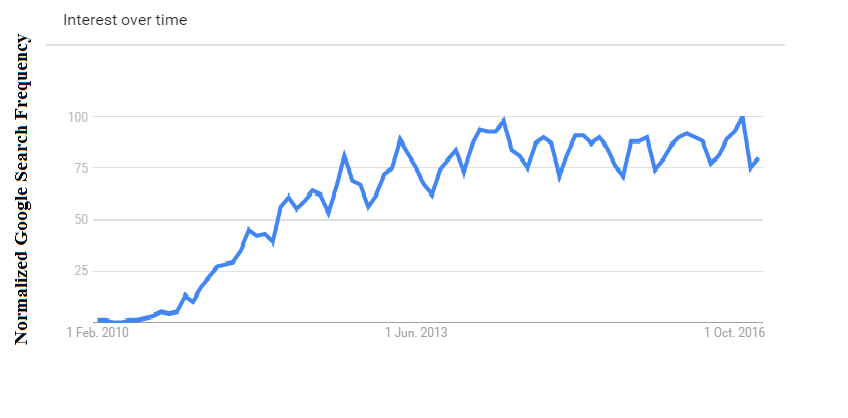
\includegraphics[width=\textwidth]{buzz}
    \caption{Google search frequency of the term \textit{gamification} from Janauary 2010 through January 2017. Data source: Google Trends, www.google.com/trends}
    \label{fig:buzz}
\end{figure}\\
Gamification is being used and studied in various domains, from education and academic performance to health care, finance, company culture building and recruitment, to name a few \cite{gamificationExamples, gamificationWiki, enterpriseGamify}. Large companies like Nike \cite{nikePlus}, Deloitte \cite{deloitte}, Starbucks \cite{starbucks}, Coca Cola \cite{coke} and Toyota \cite{toyota} have all used gamified solutions in order to increase customer loyalty, change behaviors, 
and drive innovation. Gamified solutions for sports activities are LLLLLLLL also.  %OVO TU DOTERAJ ZA STRAVE example u STUFF
Moreover, there is an increasing number of startups (e.g. Foursquare, CodeAcademy) that have gamification  at  their  core \cite{codeacademy} or offer assistance to enterprises to gamify their existing services (e.g. Badgeville \cite{badgeville}). Hamari \textit{et al.} (2014) reported on an increasing popularity of gamification related researches in the academia \cite{hamari2014does}. Figure \ref{fig:pub} gives an overview of the increase of writing on this topic. The figure includes only the number of publications for every year for the term \textit{Gamification} and excludes patents and citations. 
\begin{figure}[h]
    \centering
    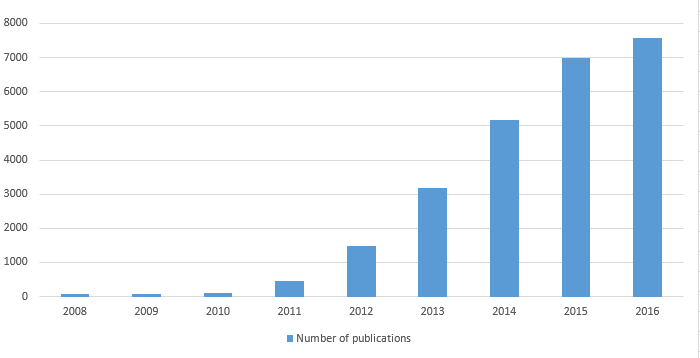
\includegraphics[width=\textwidth]{pub}
    \caption{Search hits on 'Gamification'. Data source: www.scholar.google.com}
    \label{fig:pub}
\end{figure}
It is worth noticing that the appearance of the term Gamification titles of publication has been increasing more rapidly than search hits for the same term (see Figure \ref{fig:buzz}). This suggests that Gamification is becoming more popular in academic circles as a research topic.%read fred's comments on this 
\paragraph{A Primer in Exergames}
Recent progressions in ubiquitous technologies offer a solution that could dispute a number of potential barriers preventing individuals to engage in regular physical activities. This solution comes in a form of video games that are developed for a certain purpose other than entertainment alone, mainly for the context of health and fitness, named \textit{exergames}. Compared to the term gamification, the term exergame or \textit{exergaming} has been known for a while, and its roots can be found in games released in the late eighties. The name exergame is a concatenation of the words exercise and game, sometimes referred to as \textit{Active Video Gaming} (AVGs) \cite{altamimi2012survey}. This genre includes video games with the aim of encouraging and facilitating physical activity which rely on technology that tracks body movement or reaction \cite{altamimi2012survey}. A large amount of research has been put into exergames development, and there exist several successful commercial
products today. The Nintendo Wii, released in November 2006 for the home entertainment market,
was the first mainstream game console which contained a built in exergaming system. Nintendo Wii exergame contributed to a
73\% increase in Nintendo's net sales, with 24.5 million consoles and 148.4 million software units sold to date (Nintendo, 2008), making it the second highest selling video game in 2007.%citiraj!!!  
Apart from exercise, exergames have been used in fields such as art, education, rehabilitation  \cite{altamimi2012survey}. Researches found the the usage of exergames in these fields has led to the 
development of skills such as educational skills and social skills \cite{altamimi2012survey}. 
Moreover, one important skill that exergames can
build on is children's motor skills \cite{delgado2009low}. Taking into account all the mentioned benefits one can gain with exergames, it is understandable that there is an increase of writing on this topic (see 
Figure \ref{fig:pubEx}). As in the former figure, this one also includes only the number of publications for every year for the terms \textit{exergame} or \textit{exergaming}and excludes patents and citations. 
\begin{figure}[h]
    \centering
    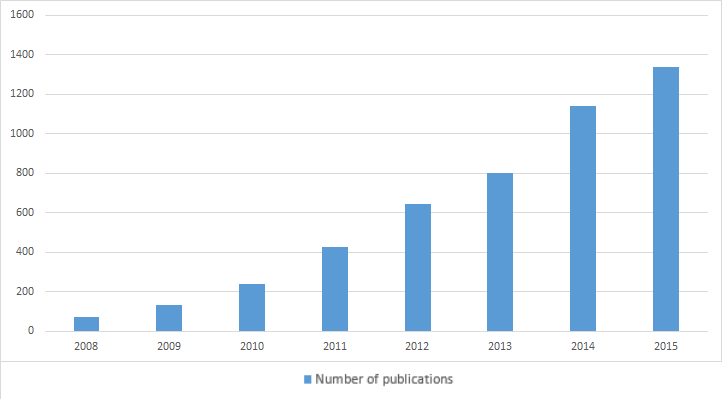
\includegraphics[width=0.9\textwidth]{pubEx}
    \caption{Search hits on 'exergame' or 'exergaming'. Data source: www.scholar.google.com}
    \label{fig:pubEx}
\end{figure}
By breaking down the barriers to traditional exercise and work-outs, exergames have the potential to promote physical
activity and stimulate behavioral change, within a fun, enjoyable and motivating context.
\section{Gamification vs Exergames}

\pagebreak
\section{Theories of Motivation}
The player forms the root of Gamification and, in any system, the outcome is affected and driven by his motivation (Zichermann \& Cunningham, 2011, p. 15). Therefore, to understand the potentials and fundamental aspects behind Gamification, one important part is to understand what drives people's motivation. Thus, psychology is  essential  to  Gamification  in order to understand  how  human  nature  works  and  how  it can  be  influenced  in  order  to  create  an  effective  Gamified  system. For this reason, the next sections introduce different views from psychology about motivation and explain what has to be considered in terms of truly engaging individuals. There are two main purposes of this section. The first is to provide a suitable overview of the subject itself and to introduce terms that will be used later in the discussion. The second purpose is to present theories that describe and explain various psychological effects that games have on players and how can they be used to enhance user's engagement and motivation when interacting with a gamified system. Two important theories that are regarded as important foundations for  the  concept of Gamification are presented. First, the Self Determination theory introduced by Ryan and Deci, and then the State of Flow by Mihaly Csikszentmihalyi are discussed. 

\subsection{The Rules of Motivation}
Gamification is about motivating  individuals to act in a certain way, or at least develop an inclination for specific behavior,  whether  it's  visiting  the gamified  system  more  often,  learning a new language, or exercising more. 
The word \textit{motivation} originates from Latin \textit{motivus} and stands for ``serve to move''. In other words, motivation can be interpreted as \textit{to be moved to do something}. It can be defined as ``those forces within an individual that push or propel him to satisfy basic needs or wants'' \cite{pardee1990motivation}. One of the most influential researchers in the domain of human motivation and behavior, Richard M. Ryan \& Edward L. Deci (2010b), argue that people \textit{can be moved} to act by various types of factors, as so with highly diverse experiences and consequences. For example, people can be motivated because they value the activity they perform, or because there exists some external influence and pressure. Furthermore, they point out that each person has different amounts and also different kinds of motivation. That is, each person is different in level (i.e. how much motivation) and orientation (i.e. what type of motivation) of their motivation, whereas orientation might be a goal which gives rise to action and therefore governs human behavior. \\*

\subsection{Self Determination Theory}
%deci ima dva papera
An aspect to understanding player motivations is by questioning the source of one's motivation. One of the most influential motivational theories is the Self Determination Theory (SDT) introduced by Ryan \& Deci (add reference). It is an empirically derived theory of human motivation that makes distinctions between different types of motivation in terms of reasons and goals that cause the respective action. That is, SDT proposes that behaviors that are intentional might vary in the extent to which they are \textit{self-determined} versus \textit{controlled}. This means that behaviors can vary in the extent they are experienced as being freely chosen and coming from one's self in contrary to being pressured or controlled externally. When these behaviors are experienced as freely chosen they are considered self-determined or autonomous, whereas the extent they are experienced as coerced, they are considered controlled \cite{deci1994promoting}. Having this in mind, SDT distinguishes between \textit{Intrinsic} and \textit{Extrinsic} motivation. The first type of motivation, as the word \textit{intrinsic} already suggests, refers to performing an activity for the inherent satisfaction. When intrinsically motivated, a person is moved to act because the activity is challenging, interesting and enjoyable on its own rather than because of some external prods, pressures, or rewards. On the other hand, extrinsic motivation refers to performing an action because it leads to \textit{separable outcome}. That is, there is some external reward or influence which drives the person to accomplish the task (Deci  \& Ryan, 2000). The comparison between people intrinsically and those extrinsically motivated reveals that the former have more interest, excitement, and confidence which in turn, can not only enhance performance, persistence, and creativity but consequently boost vitality, increase self-esteem and general well-being \cite{ryan2000self}. Though this division is for most people intuitively understandable, it is not always as clear as it may seem. For example, as the SDT theory states, \textit{motivations are fluid}. Hence, people can convert extrinsic motivators to intrinsic if they internalize the desire to do so. To put it more simply, in a situation where the extrinsic motivator is found meaningful, pleasurable and consistent with a person's worldview, it can be perceived and adopted as if it was intrinsic \cite{zichermann2012}.
Although, in one sense, intrinsic motivation can exist within an individual, in another sense, it can exist in the relation between the individual and the activity one performs. Having that in mind, it is important to point out that not everyone is intrinsically motivated for the same activities and that not everyone is intrinsically motivated for any particular activity \cite{ryan2000intrinsic}. In SDT, the \textit{basic psychological need satisfaction} is assumed to be the core motivational mechanism that directs human's behavior. SDT postulates three innate psychological needs (see Figure \ref{fig:ss} ), that are ``essential for ongoing psychological growth, integrity, and well-being'' and all three of them play a necessary part in optimal development, hence none can be disregarded without significant negative consequences. These needs are the need for autonomy, competence and relatedness. When individuals experience them, they become self-determined and intrinsically motivated to pursue things that interest them the most \cite{deci2000and}. %https://selfdeterminationtheory.org/SDT/documents/2010_VandenBroeckVansteenkisteNSscale_JOOP.pdf
\begin{itemize}
\item \textbf{Autonomy} represents individuals' innate desire to feel \textit{free} and to experience a sense of choice and psychological freedom when carrying out certain activities \cite{deci2000and}. Situations in which individuals are provided with the opportunity to choose freely, accompanied with a positive feedback, have been shown to influence and improve autonomy and, hence, the intrinsic motivation of individuals [ryan 2006]. For example, students  are  autonomous when they willingly spend time and energy for completing their assignments. 
\item \textbf{Competence} represents individuals' innate desire to feel effective when interacting with the environment. For example, students are competent in cases when they feel they can meet the challenges of their schoolwork. Furthermore, Deci \& Ryan (2000) point out that positive feedback can signify effectance and provide a satisfaction of the need for competence, thus enhancing intrinsic motivation, whereas negative feedback that convey ineffectance, tend  to
diminish the sense of competence and hence undermine intrinsic motivation. 

%A. P. Hill, "A Brief Guide to Self-Determination Theory," September 2011. [Online]. Available: http://www.heacademy.ac.uk/assets/hlst/documents/projects/round_11/r11_hill_guide.pdf. [Accessed 10 April 2013].

\item \textbf{Relatedness} corresponds to experiencing meaningful connection to others, that is, to be a member of a group, to love and care and to be loved and cared for \cite{broeck2010capturing}. This psychological need is satisfied when individuals experience a sense of togetherness and develop a close and intimate relationship with others.
\end{itemize}
\begin{figure}[h]
    \centering
    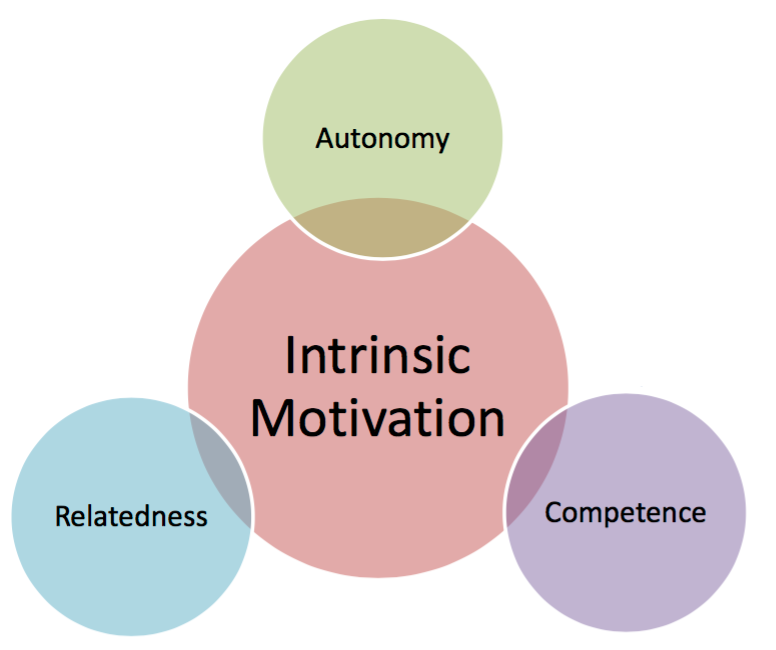
\includegraphics[width=0.6\textwidth]{ss}
    \caption{Basic psychological needs according to Ryan, R.M. \& Deci E.L. \cite{deci1994promoting} }
    \label{fig:ss}
\end{figure}
The specification of autonomy, competence, and relatedness is important because it allows the prediction of variables that can affect individual's intrinsic motivation and the development of their extrinsic motivation \cite{deci1994promoting}. These needs can be achieved by means of diverse game elements, which will be discussed in detail in the next section.\\*\\*
Despite the observable evidence that humans, in general, can have intrinsic motivational tendencies towards some activities, this bias appears to manifest only in certain conditions and circumstances. Hence, SDT also places much emphasis on understanding conditions that enhance and sustain versus subdue and diminish intrinsic motivation.  A sub-theory of SDT called Cognitive Evaluation Theory (CET) was presented by Deci and Ryan (1985) and focuses on social and environmental factors that promote or undermine this type of motivation using language that reflects the assumption that intrinsic motivation, as an inherent bias, is rather catalyzed than caused when individuals are in appropriate socio-enviromental circumstances (Ryan  and  Deci  2000;  Ryan and Deci 2000b). In other words, intrinsic motivation does not occur by itself, but represents the outcome of one's interaction with the environment and one's interests and preferences. That is, intrinsic motivation ``will flourish if circumstances permit'' \cite{ryan2000self}. Furthermore, CET, which focuses mainly on the fundamental needs for competence and autonomy, argues that interpersonal events and structures, such as rewards, communication or feedback can increase intrinsic motivation for certain actions because they satisfy the basic psychological need for competence. Accordingly, it is predicted that optimal challenges, positive feedback and freedom from degrading evaluations promote intrinsic motivation, while tangible rewards, threats,  deadlines  and  directives decrease it (Ryan \& Deci, 2000). Furthermore, CET also argues that the satisfaction of the psychological needs for competence will not enhance intrinsic motivation unless they are joined by a sense of autonomy. Hence, people must perceive that their behavior is self-determined in order for intrinsic motivation to be maintained or enhanced. In other words, for a high level of intrinsic motivation, the needs for competence and autonomy must both be satisfied (Ryan \& Deci, 2000). It is important to point out, as stated by Ryan \& Deci, that people will be intrinsically motivated for certain activities only when they are intrinsically captivating for an individual, that means activities that offer a degree of novelty, challenge or aesthetic value. Activities that do not provide such appeal, will not be experienced as intrinsically motivated. \\*
Even though intrinsic motivation is of great importance, most of the activities people engage in are not intrinsically motivated. Such activities, being uninteresting and unsatisfactory for individuals  require external \textit{push} in order to be realized. This motivation, contrary to intrinsic motivation which refers to doing an activity simply for the enjoyment of the activity itself, is known as extrinsic motivation. It refers to performing certain activities because it is expected to result in some additional outcome or reward that have an instrumental value for the individual performing that action \cite{ryan2000self}. In general, extrinsically motivated behaviors are ones that would not happen instinctively, and hence must be prompted by an intrumentality \cite{deci1994promoting}. Various studies demonstrated that in specific circumstances extrinsic motivation can sustain intrinsic motivation, thus suggesting that extrinsically motivated behaviors can also be self-determined \cite{deci1994promoting}. Extrinsically motivated behaviors become self-determined through the process of \textit{internalization} and \textit{integration}. Internalization involves transforming internal regulatory processes into internal regulatory processes, while integration corresponds to the process of integrating these now internalized values and regulation into one's self \cite{deci1994promoting}. There exist four types of extrinsic regulation that can result from different types of internalization and integration, which were introduced within SDT as a subtheory called Organismic Integration Theory (OIT) \cite{ryan2000intrinsic, ryan2000self, deci1994promoting}. For instance, students who work on their assignments because they personally understand its importance for their future career and those who do it only to adhere to their parents' control are both extrinsically motivated. Even though both cases involve instrumentalities rather than enjoyment, the former entails personal endorsement and a feeling of choice while the latter associates only with an external regulation.\\*
Figure \ref{fig:tax} illustrates the IOT taxonomy of motivational types arranged from left to right in terms of the degree to which the motivation originates from the self (i.e. are self-determined). 
\begin{figure}[h]
    \centering
    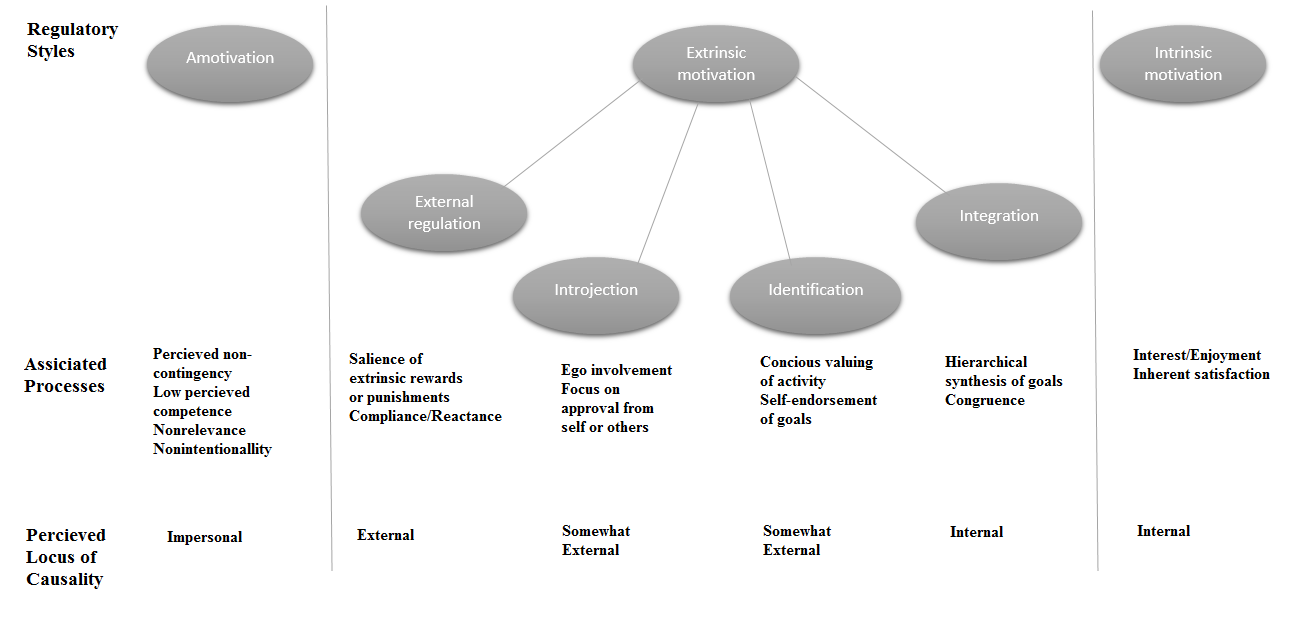
\includegraphics[width=\textwidth]{taxm}
    \caption{Based on Ryan, R.M. \& Deci E.L. Self-Determination Continuum showing types of Motivation}
    \label{fig:tax}
\end{figure}
First, the extrinsically motivated behavior that is the least autonomous is known as \textit{External Regulation} and is regulated through some external means, such as rewards and constraints. For example, an athlete who participates in the Olympics only to obtain a medal represents an instance of externally regulated behavior. In case of \textit{Introjected regulation}, individuals begin to internalize the reasons for their action. However, this internalization only replaces the external source of motivation with an internal one, such as guilt, worry or shame. That is, when people are motivated to perform activity in order to maintain feeling of worth. An example for introjection is the athlete who goes to the practice just because he would feel guilty if it has been skipped. A more autonomous type of extrinsic motivation, \textit{identification}, manifests when a person identifies with the importance of some behavior and accepts it as a personal regulation only because it benefits the athlete in achieving a specific goal. An example for this behavior is a runner who does not like weight lifting, but nevertheless chooses to to do it because it will positively impact her future performance. \textit{Integrated regulation}, as the most autonomous of extrinsic motivation that shares many qualities with intrinsic motivation, is a form of motivation that arises when an individual has fully assimilated the identified regulation within himself. An example of integrated regulation is an athlete who chooses to postpone the night out with his friend in order to be in good shape for the next day's tournament. Integration together with intrinsic motivation represent the core for self-determined functioning and they both share the qualities that constitute self-determination. Even though they might seem quite similar, they are different in the sense that intrinsically motivated behaviors are ``autotelic in nature'' while, on the other hand, integrated behaviors are ``instrumentally (though freely) performed'' for the outcome that is self satisfactory.  Finally, the self-determination continuum is closed with  \textit{amotivation} which represents ``non-regulation'' from the SDT perspective as it refers to a state where intentions to act are non existent. A person amotivated towards exercise would not exercise at all, 
or engage in exercise in a passive and disorganised  manner \cite{vallerand2007intrinsic, ryan2000intrinsic, deci1994promoting}.

\subsubsection{Gamification and SDT}
In their book \textit{For the win. How Game Thinking can revolutionize your business} (2012 )\cite{werbach2012win} Werbach and Hunter state that ``games are perfect illustration of the lessons of SDT''. They point out how even simple games activate intrinsic needs for autonomy (because it is up to the player how to solve a challenge), competence (sense of accomplishment if certain goal is achieved) and, lastly, relatedness (when the the achieved results are shared among group of friends). The same way as games, Gamification uses these three innate motivators in order to generate results.
What are the specific takeaways for a successful gamification?
- Rewards can crowd out fun
- Boring can be engaging
- Tune your feedback
Tangible and expected extrinsic rewards can damage intrinsic motivation and interesting tasks (Werbach and Hunter,2012, p.60). On the other hand, extrinsic rewards can also have a positive effect when people need to accomplish boring
tasks (Werbach and Hunter,2012, p.62).
NOT COMPLETED-TODO:add relation to the warm up scenario? how do we plan to address autonomy, relatedness and competence? 
\\*

\subsection{State of Flow}
TODO: is the state of flow realistically achievable in 15 minutes or short intervals? to argue. so you need to look into how much time is needed to reach this state?

Mih\'{a}ly Cs\'{i}kszentmih\'{a}lyi, one of the most recognized game psychologists and a professor at University of Chicago, described in 1975 for the first time the phenomenon of \textit{flow}. Being fascinated by artists who would essentially get lost in their work Cs\'{i}kszentmih\'{a}lyi argued how, creative people might differ from one another in many ways but they always have one thing in common. They love what they do. Their love for a particular activity is not because of a potential outcome or a reward. What drives them is solely the opportunity to do what they enjoy doing \cite{csikszentmihalyi1996flow}. Athletes often refer to this concept as ``being in the zone,'' religious mystics
as being in ``ecstasy,'' artists and musicians as ``aesthetic rapture'' \cite{csikszentmihalyi1997finding}. In order to explain this experience, Cs\'{i}kszentmih\'{a}lyi has interviewed individuals willing to devote many hours to their avocations without asking for external rewards. After a series of studies, based on the individuals' responses regarding their emotions while performing certain activity they enjoy, Cs\'{i}kszentmih\'{a}lyi  developed a theory of optimal experience based on the concept of \textit{flow}, which he describes as 
``the state in which people are so involved in an activity that nothing else seems to matter; the experience itself is so enjoyable that people will do it even at greater cost, for the sheer sake of doing it'' \cite{flow1990psychology}. Flow is also considered as an optimal state of intrinsic motivation, where people become absolutely immersed in what they are doing, they forget about physical feelings, passage of time, and their ego fades away \cite{lithiumGamification}. 
It represents a state in which one feels in control, fully immersed and motivated, at the top of its abilities and neither overwhelmed by difficulty nor uninterested. Cs\'{i}kszentmih\'{a}lyi \textit{et. al} (2004) state the flow experiences are relatively rare in everyday life, however, various activities are able to produce them, provided certain conditions are met. They further argue that three conditions have to be met in order to achieve a flow state. First, a state of flow needs clearly defined set of goals which must guide the user and give purpose to the behavior \cite{csikszentmihalyi2014flow}. However, sometimes the goals of some activities cannot be perfectly clear for the individual, as in the case of creative activities. Nonetheless, it is possible for a person to develop a strong personal sense of what is intended to be done by performing the activity \cite{kiili2006evaluations}. The second condition for obtaining the state of flow is the presence  of clear and immediate feedback. It informs the user if he/she is succeeding in a specific goal and how to adjust his or her performance according to the ``continually  changing environment demands'' \cite{csikszentmihalyi2014flow}. Lastly, one of the most important condition is to maintain balance between perceived challenges and perceived skills \cite{csikszentmihalyi2014flow}. When experiencing a flow, a person's skill is at just the right level to cope with the situational demands.\\*
Nakamura and Cs\'{i}kszentmih\'{a}lyi (2012) further argue that under these three conditions, individuals can enter a state with the following characteristics:
\begin{itemize}
\item Control. A sense that one has skills sufficient enough to minimize the margin of error to close to zero and, therefore, can in principle deal with and fully enjoy the current situation because one knows how to respond to any anything that can happen next \cite{csikszentmihalyi2014flow}. Moreover, this sense of control is believed to be one of the important flow antecedents in games\cite{kiili2006evaluations}. 
\item Action–awareness merging. The flow state is so involving that, during it, it affects the individual in a way that the activity performed becomes spontaneous and automatic.
\item Concentration. While in flow, one experiences intense and focused concentration on what is being done in the present moment. By doing so, one is able to forget all unpleasant things beyond the performed activity since the person is left with no cognitive resources for irrelevant information processing \cite{kiili2006evaluations}. 
\item Loss of self-consciousness. During flow, the self disappears from one's awareness. That is, while thoroughly engrossed with an activity, as in the state of control, few cognitive resources are
available for self-scrutiny \cite{kiili2006evaluations}.
\item Distortion of temporal experience. Typically, the sense of time
during the flow experience tends to bear little relation to the actual passage of time, a
sense that time has passed faster than normal.
\item Autotelic experience. Autotelic experience refers to an activity that is performed simply because it is intrinsically rewarding and not with the expectation of some future benefit.
\end{itemize}
Whenever individuals try to reflect on their flow experiences, they tend to mention some and often all of these characteristics. The described conditions and characteristics of flow are known as the \textit{nine dimensions of the state of flow}, where the first five dimensions can be considered flow antecedents and the rest indicators of flow experience  \cite{kiili2006evaluations}.
According to Cs\'{i}kszentmih\'{a}lyi, flow often tends to occur in situations when we face challenges that match our skills and abilities. That is, it occurs when we perform tasks and activities that are neither too difficult nor too easy with respect to the set of skills we possess - a balance of the relationship between challenge and ability \cite{csikszentmihalyi1997finding, flow1990psychology, csikszentmihalyi1996flow}. This balance is referred to as \textit{flow zone}. When the task is too difficult (i.e., the skill cannot meet the challenge), that is when one is above the flow channel, we are likely to experience anxiety. In the opposite case, when the task is slightly too easy and task challenges do not come close to our ability, the result is boredom. Furthermore, if a person's skills improve over time, the challenge difficulty also needs to increase along with the improved skill-set. Figure \ref{fig:flowZone} depicts the graphical representation of the state of flow, where y-axis represents the difficulty of the challenge and the x-axis skill set required to meet the specific challenge. Moreover, diagram contains the flow-channel, as well as the anxiety-region and the boredom region. 
\begin{figure}[h]
    \centering
    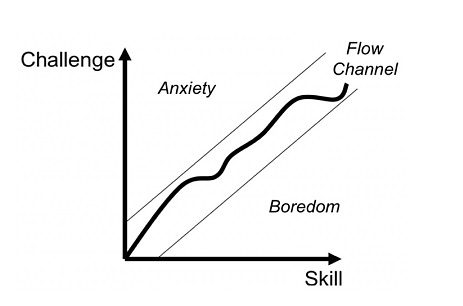
\includegraphics[width=0.6\textwidth]{flowZone}
    \caption{Based on the original model of the flow state)}
    \label{fig:flowZone}
\end{figure}
Over the years, new theories regarding the state of flow have been introduce and the concept flow was redefined by introducing eight experimental channels rather than previously mentioned quadrants \cite{nakamura2014concept}. Figure \ref{fig:flowModel} shows the refined challenge/skill space which now contains a series of concentric rings, associated with increasing intensity of experience.
\begin{figure}[h]
    \centering
    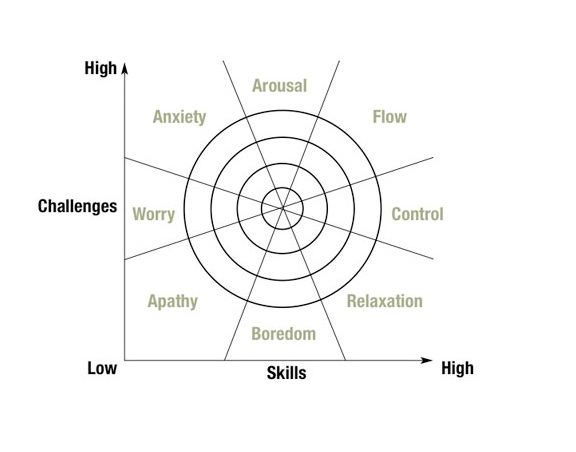
\includegraphics[width=0.6\textwidth]{flow-model}
    \caption{The current model of the flow state \cite{nakamura2014concept}}
    \label{fig:flowModel}
\end{figure}
Based on the current model of the flow state \ref{fig:flowModel}, the flow is experienced in situation when challenges and
skills are above the individual's average levels. When the task is slightly too easy (or slightly too hard) we fall out of the state of flow and enter a state where we feel in control (or the state where we feel aroused if the task is slightly too hard). When the difficulty of the task performed way above our skills, we are tend to experience anxiety. On the other hand, if challenges do not come close to our ability, we will tend to experience boredom. In cases they are below, apathy is experienced. The new model also deals with the intensity of the experience and states the it increases with distance from the individual's average levels of challenge and skill, as shown by the concentric rings \cite{nakamura2014concept}.
Cs\'{i}kszentmih\'{a}lyi \textit{et al.} (2004) also argue how sports and games are more likely to lead to a flow state since they usually have clear goals and feedback structures. However, a given individual can find flow in almost every activity that for some other individuals might seem boring or tiresome \cite{csikszentmihalyi2014flow}.

\subsubsection{Flow in Gamification}
In the context related to human behavior and computers, the concept of flow has been mostly studied in video games, human-computer interaction, instant messaging, to name a few \cite{hamari2014measuring}. Currently, there exist only few studies investigating flow in the context of Gamification (see \cite{hamari2014measuring, sillaots2014achieving}). Thus, and there is insufficient data to draw conclusions as to which of the nine dimensions of flow would be especially emergent in the context of flow. To this end, Hamari and Koivisto (2014) conducted a study in which they investigated the influence and importance of the different dimensions of flow in Gamification.  The data for this study was gathered from users of an exercise gamification service (N = 200) and as a measurement instrument for flow, the Dispositional Flow Scale - 2 (DFS-2) model was used. Introduced by Jackson and Eklund (2002), DFS-2 is designed to access flow experiences in physical activity (see \cite{jackson2002assessing}). The results showed that autotelic experience, clear goals, (immediate) feedback, control and challenge-skill balance were the most salient dimensions of flow in Gamification (of exercise). On the other hand, time transformation, merging action-awareness, loss of self-consciousness were the least salient as shown in Figure \ref{fig:dfs2}.
\begin{figure}[h]
    \centering
    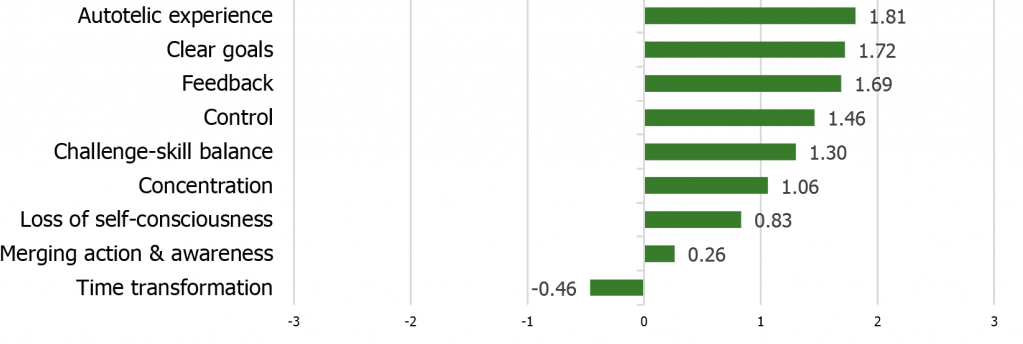
\includegraphics[width=\textwidth]{dfs2}
    \caption{Measuring flow in Gamification: Dispositional Flow Scale-2. Source:  \cite{dfs2}}
    \label{fig:dfs2}
\end{figure}
Furthermore, results also suggest that in gamifed context, the autotelic experience is highly correlated with the conditions. Hamari and Koivisto suggest that it is possible that in the Gamification context, autotelic experience truly represents a condition for reaching flow, thus implying that one can more easily reach flow if the activity is initially intrinsically motivating. 
\subsection{Motivation and Sports}

%pelletier1995toward
Vallerand (2004) states that motivation in sports matters, as it ``represents one of the most important variables in sport''. It is known to be a key element of success in sport and athletes' persistence with an exercise regiment \cite{vallerand2007intrinsic}. Intrinsic and extrinsic motivation have been particularly popular topics that allowed researchers to explain various phenomena of importance in sport and physical activity. Various studies in the domains of health, physical education, exercise and sport have explored the SDT derived hypothesis that intrinsically relative to extrinsically motivated behavior  
TODO: in which areas gamification in sports works already? are there theory parts results that are applicable to our work?...\\*\\*
Armed with a clear understanding of the theory behind human motivation, the following section begins by defining the term Gamification. The goal of this section is to provide an overview of the most relevant key elements of Gamification relevant for the development of iMMotion, in particular why certain game mechanics were the best choice for the iMMotion project.
%In recent years gamifi cation systems were applied in marketing(Muntean, 2011 ; Shneiderman, 2004 ) as well as non-business contexts such as politics,health (Lee & Hammer, 2011 ), or interactive systems (Flatla, Gutwin, Nacke, Bateman,& Mandryk, 2011 ) and education (Lee & Hammer, 2011 ; Raban & Geifman, 2009 ;Rafaeli, Raban, Ravid, & Noy, 2003 ; Ravid & Rafaeli, 2000 ). This rapid developmenthas caught the interest of researchers as a potential to create engaging workplaces(Reeves & Read, 2009 ); facilitate mass-collaboration (McGonigal , 2011 ) or encourageknowledge contribution (Krause & Smeddinck, 2011 ; Shneiderman, 2004 ; von Ahn &Dabbish, 2008 ).
\subsection{Defining Gamification}
As  the  term  itself  is  relatively  new,  there  exist  numerous definitions  of  Gamification  (Zicherman \&  Cunningham 2011, Kapp 2011, Werbach \& Hunter 2012). Definition by Deterding \textit{et al.} (2011) is currently the most cited definition of Gamification in academia and is the definition that is adopted for this thesis. In their paper the authors proposed a well reasoned definition as follows:
\begin{quotation}
\textit{``Gamification is the use of game design elements in a non-game context.''}
\end{quotation}
There exist references to \textit{gamifying} online systems as early as 1980. Professor Richard Bartle from University of Essex, points out the word referred originally to ``turning something not a game into a game.''\cite{werbach2012win}%ovo je knjiga, daj stranu 
However, the first use of gamification in its current sense dates back to 2002 by Nick Pelling as part of his consultancy business, but the term did not see widespread adoption before the second half of 2010 \cite{marczewski2013gamification}. In parallel with this term, a verb \textit{to gamify} emerged. Its meaning refers to applying game mechanics to supercharge user engagement, loyalty and fun \cite{toGamify}. 
It should be noted that the definition outlined by Deterding \textit{et al.} relates to \textit{games} and not \textit{play} \cite{deterding2011game}. %Consequently, the definition distinguieshes between \textit{gamefullness} and \textit{playfullness} ... TODO. 
Even though often used interchangeably, there exists a complex relationship between these two concepts and clear distinction can be made. That is, according to the forms they take in the world, \textit{play} can be interpreted as a broader category that includes \textit{game} as a subset \cite{salen2004rules}. Play is normally assumed to be a free-form activity lacking constraints engaged in for pleasure and amusement rather than a serious or practical purpose, whereas games provide context for actions and are limited in action by fixed rules \cite{juul2011half}. In addition, Salen \& Zimmerman (2004) define game as a system where players engage in an artificial conflict which is defined by rules that limit player's behavior and define the game, that can result in a quantifiable outcome or goal \cite{salen2004rules}. %behavioral, game-playing
Games manifest themselves as integrated experiences, but they are built from many smaller pieces often called game elements \cite{werbach2012win}. They represent parts of games used as a building blocks for creating gamified applications, as well as tools and rules that define the overall context of game \cite{gamDesElem}. This means that the definition distinguishes Gamification from other systems that employ full-fledged games rather than elements of game design only. Furthermore, it does not include all game elements either, only a subcategory called game design elements that are used as seen the most suitable in current situation. %ova dve poslednje recenice odavde, izmeni 
%http://ludus.hu/en/gamification/
The final aspect of the definition is that gamification operates in non-game contexts. A non-game context refers to applications which main purpose is beyond pure entertainment; using game design elements to a context of ``other than games''. This implies that gamification can be used and successfully applied to almost anything: from business, finance, personal improvement to education, health and fitness \cite{deterding2011game}. Thus, the challenge of Gamification, is to select elements that normally operate within the game universe and apply them effectively in the real world.
\begin{figure}[h]
    \centering
    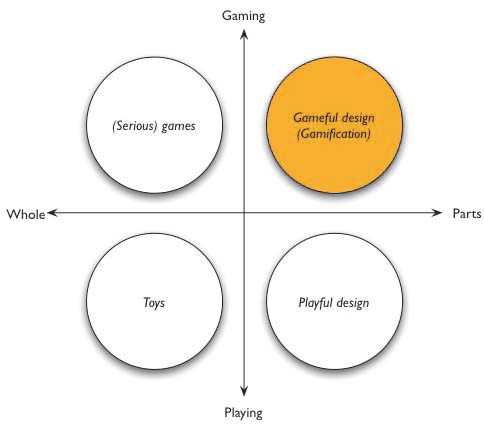
\includegraphics[width=0.75\textwidth]{gamification-btw-game-and-play}
    \caption{The matrix distinguishing the concepts related to gamification}
    \label{fig:mesh1}
\end{figure}
The concept of gamification is closely related to similar pre-existing concepts such as serious games, playful design and toys. Thus, the proposed definition aims at separating the concept of gamification from similar phenomena on a two-by-two matrix introduced by Deterding \textit{et al} (2011, Figure \ref{fig:mesh1}). 
In figure \ref{fig:mesh1}, along one axis a distinction between gaming and playing is made, and on the other between whole game and an artifact with game elements. Gameful design or gamification, differs from playful design because the former focuses on activities that are goal oriented and structured by rules, while the latter focuses on activities that are based on improvisation and are free of form. Moreover, gamification is situated in the quadrant involving games and game elements, meaning that gamification makes use of gameful design rather than playful design and game elements rather than full-fledged games. This is different to serious games used also in non-game contexts, a group that includes full games that have been created for reasons other than pure entertainment. 
\subsection{Defining Exergames}
According to Matallaoui \textit{et al.} (2017), ``one of the most prominent fields where
gamification and other gameful approaches have been
implemented is the health and exercise field'' \cite{matallaoui2017effective}. Even though known for decades, due to the technological advancements which allow more widespread and affordable usage of motion based controllers, these gameful systems and approaches that involve physical activity as the means of interacting with the game, commonly known as \textit{exergames}, have only been proliferating 
in recent years \cite{matallaoui2017effective}. 
According to XXX, the main reason for increased interests in exergames is the concern over high levels of obesity in Western society. Apart from high calorie diet, physical inactivity is considered to be the main reason for obesity, especially among children \cite{kiili2010developing}. Since playing video games is a common leisure time activity among people of all ages, it has been argued by many researchers \cite{kiili2010developing} that video games are one of the main reasons for the decreased level of everyday physical activity and hence, increased level of obesity \cite{vandewater2004linking}. This is what the emerging exergames genre tries to change by encouraging players to perform physical movements during gameplay \cite{kiili2010developing}. Exergames can be defined as ``video games that require physical activity in order to play'' \cite{oh2010defining}. However, a more precise definition of exergame is given by Oh and Yang:
\begin{quotation}
\textit{``An exergame is a video
game that promotes (either via using or requiring) players’ physical movements (exertion) that is
generally more than sedentary and includes strength, balance, and flexibility activities.''} \cite{oh2010defining}.
\end{quotation}
The authors also define exergaming as an: 
\begin{quotation}
\textit{``experiential activity where playing exergames, videogames, or computer-based is used to promote physical activity that is more than sedentary activites and also includes strength, balance,
and flexibility activities''} \cite{oh2010defining}.
\end{quotation}
They main goal is to motivate people to exercise by providing a  ``safe, entertaining and engaging fitness atmosphere'' \cite{altamimi2012survey}.


Researcher at ... showed the exergames can also be used as a fitness tool to help improve and increase the fitness level
The author in [55]
demonstrated this idea using his own body as the main subject
of his experiment. He played three active video games which
differed in the interactions they involved. The three active
games that were used were Dance Dance Revolution which
requires the full body interaction, the EyeToy games which
mainly require upper body interaction and GameBike games
which utilize lower body interaction. After three months of
daily 30 minute sessions plays, two benefits were observed by
the author; weight loss and blood sugar level reduction
\subsection{Player Types}
An important aspect of game thinking is that players differ from one another and their motivation for engaging in gaming activities should not be generalized. That is, people choose to play games for different reasons, and thus, the same video game can have a different meanings or consequences for different players \cite{yee2006motivations}. The more is known about who is playing the game, the easier it is to design and implement an experience that will drive players' behavior in the desired way \cite{zichermann2011gamification}. The  remainder  of  this section will further explore premises about player behavior and personality types. 

\paragraph{Bartle's Four Player Types}

One way to understand players' motivation is to leverage the work accomplished by Richard Bartle in examining player types. Bartle conducted researches in the area of game design and game development and analyzed the ethnography of online game players in the first MUD in 1978 (Multi-User Dungeon). In order to understand why people play games, he identified four main player personality types of MUDs according to specific psychological aspects of their personality and how they prefer playing in a virtual world: \textit{Explorers}, \textit{Socializers}, \textit{Killers}, and \textit{Achievers} \cite{bartle1996hearts}. The player personality types (see Figure \ref{fig:userTypes}) can be defined as follows:
\begin{itemize}
\item \textbf{Explorers} represent players which are driven by motivation to ``find out as much as they can about the 
virtual  world'' \cite{bartle1996hearts}. Not only they enjoy exploring every corner of the game environment and searching for interesting features (i.e. bugs), but also understanding  how 
everything functions \cite{bartle1996hearts}. 
In a sense, for this type of players ``the experience
is the objective'' \cite{zichermann2011gamification}.
\item \textbf{Socializers} are player who play games for the benefit of a social interaction \cite{zichermann2011gamification}. They usually enjoy using communication tools that are provided by the game in order to engage in conversation with other players. 
\item \textbf{Achievers} are goal (achievement) oriented players. They are players who are proud of their ``formal status in the game's built-in level hierarchy'' and also ``of how short a time they took to reach it'' \cite{bartle1996hearts}. This type of players are competitive who enjoy beating difficult challenges whether they are explicitly  set by the game (e.g.  levelling  up  or  gathering  points) or by themselves (e.g. accumulating as much money possible). 
\item \textbf{Killers}, also known as \textit{griefers} \cite{zichermann2011gamification}, are the smallest population of all the player types. They are very similar to achievers, in their motivation for winning, however, these players obtain  enjoyment from causing anxiety and "imposing  themselves  on  others" \cite{bartle1996hearts}. For them, winning is only meaningful if someone else loses.
\end{itemize}
\begin{figure}[h]
    \centering
    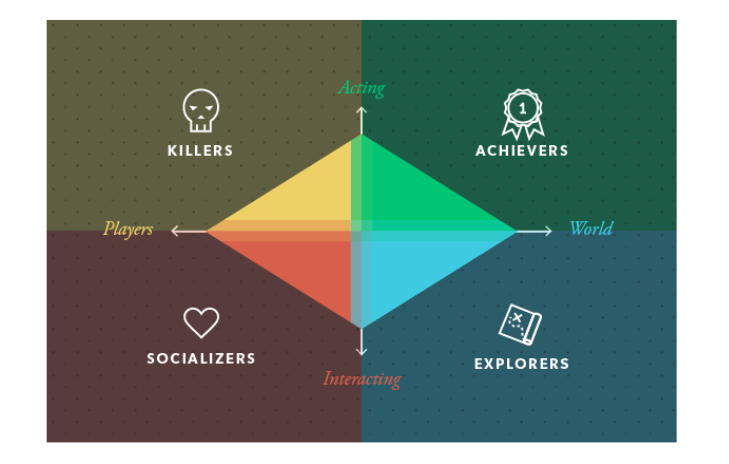
\includegraphics[width=0.75\textwidth]{userTypes}
    \caption{Bartle's Taxonomy of Player Types. Source \cite{bartle}}
    \label{fig:userTypes}
\end{figure}
In the above figure, axes represent the source of players' interest in a MUD. The horizontal axis depicts a preference for interacting with other players vs. interacting with the world and the vertical axis represents a preference for (inter)acting with something vs. (inter)acting on something. Thus, according to the figure, achievers prefer to act on the world, while socializers prefer to interact with other players \cite{bartle}. \\*
It is important to point out that people are not exclusively one or another of the presented player types \cite{zichermann2011gamification}. In their book, Zichermann and Hunter argue that most people have some percentage of each type and the most dominant type will probably change throughout the individual's life. Even though Bartle's player types have not been designed in particular for Gamification it can  help in understanding what attitudes may be dealt with when implementing a gamified solution. 

\paragraph{Marczewski's User Types Hexed}

Bartle's taxonomy of user types was created
specifically for MUDs and it should not be generalized
to other game genres nor to gameful design \cite{tondello2016gamification}. Moreover, it does not consider players who are extrinsically motivated. In order to address these issues Marczewski proposed six user types that differ in the degree to which they can be motivated by either intrinsic or extrinsic  motivational factors \cite{tondello2016gamification} and introduced the \textit{Gamification User Types Hexad framework}.
\begin{figure}[h]
    \centering
    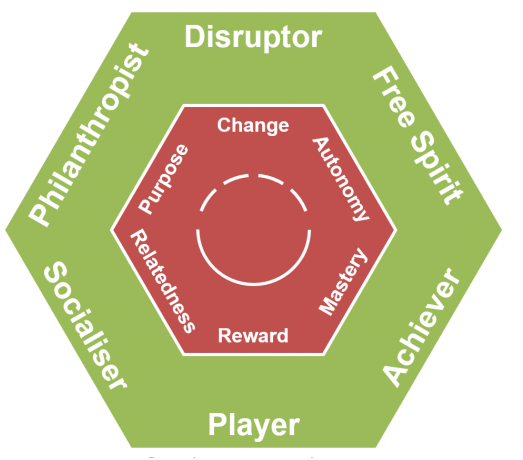
\includegraphics[width=0.75\textwidth]{playerHex}
    \caption{Gamification User Types Hexad. Source: \cite{tondello2016gamification}}
    \label{fig:playerHex}
\end{figure}
\textit{The Hexad} illustrated in Figure \ref{fig:playerHex} is developed in order to identify the users of the gamified system more efficiently, based on users' intrinsic and extrinsic motivations, as defined by SDT \cite{tondello2016gamification}. Marczewski identifies the following types:
\begin{itemize}
\item \textbf{Socialisers} are individuals motivated by \textit{Relatedness}, want to interact with others and create social connections \cite{tondello2016gamification}.
\item \textbf{Free Spirits} are individuals  motivated by \textit{Autonomy} and self-expression. They enjoy the freedom of expression and acting without any external control \cite{tondello2016gamification}.   
\item \textbf{Achievers} are individuals  motivated by \textit{Competence}. As in Bartle's taxonomy, this group seek progress withing the gamified environment by completing various tasks and enjoy proving themselves by overcoming difficult challenges \cite{tondello2016gamification}.
\item \textbf{Philanthropists} are individuals motivated by \textit{Purpose} and \textit{Meaning}. These individuals enjoy giving to others with no expectation of reward in return \cite{tondello2016gamification}.
\item \textbf{Players} are motivated by \textit{Extrinsic rewards}. Motivated only by the reward offered by the gamified system, they will do anything necessary to obtain it, independently of the type of the activity \cite{tondello2016gamification}.
\item \textbf{Disruptors} are motivated by \textit{Change}. In general, they tend to disrupt the system, either directly or through other users to force positive or negative change \cite{tondello2016gamification}.
\end{itemize}
As already mentioned, most people demonstrate each player type to a certain degree. Understanding these player types will support 
the process of choosing the game elements that will be most appealing for the target audience and drive the 
desired behavior. Furthermore, adding features and content in order to appeal to different player types can be of great help to diversify the audience of the gamified system, and create enjoyable experiences for many players.

\subsection{Gamificaton elements}
% \cite{schobel2016agony}.% Sch{\"o}bel \textit{et al.} carried out a literature review to analyze the gamification elements used in various research studies.
%prezentacija o game vs play http://gamification-research.org/2012/04/defining-gamification/
%detering definise elements of game design. five leveles.Next the most common
%Next, and overview and various classification frameworks of game elements which might further enhance engagement, the potential goal of gamification is presented. 
%In a few words, the gamification process can be described as the adoption of some techniques inherited from game design into different situa-tions, other than games. In this perspective, the application of the typical game elements and the exploitation of common game design patterns are used to the aim of making some activities more appealing. In this way, users are stimulated to complete tasks by the desire of getting some rewards (Werbach & Hunter, 2012). Hence, gamification is not related to solve difficult puzzles or avoid tricks but it is the finding of effective ways to drive individuals to their goals faster. Through gamification, people feel involved in the process and are called to be proactive so that they can empower their own abilities and enhance their attitudes both online, in virtual worlds, and offline, in real world situations. Currently, gamification is used by industries to enhance the outcome of their communication campaigns and to drive the attention of people to advertising and marketing messages, in order to maximize their outcome.To conclude, gamification requires a deep understanding of what we can learn from games, so that we can design enjoyable environments and raise passion for the game we are playing  Applying gamification techniques to enhance the effectiveness of video-lessons. Available from: https://www.researchgate.net/publication/283469412_Applying_gamification_techniques_to_enhance_the_effectiveness_of_video-lessons [accessed Mar 5, 2017].
In their book \textit{Gamification by design}, Zimmerman and Cunningham (2011) argue that one should leverage aspects of game design, by focusing on it's core elements, when creating a gamified experience in order to achieve the
greatest impact for players. However, the goal of Gamification is not to build a ``full-fledged game'' but to use game elements in order to provide a gamified experience and enrich the application to engage and motivate the users \cite{werbach2012win, deterding2011game}. With respect to the use of game elements, Gamification studies classified them differently and there have been different attempts to create lists of those game  elements,  which  can  be applied in Gamification \cite{werbach2012win, deterding2011game, kapp2012gamification, zichermann2011gamification}. Derived from the available literature, Deterding \textit{et al.} found that game elements previously identified and presented in different research studies, fell in five distinct levels of abstraction. Table \ref{table:gameElements} presents a model for classification of game elements with five levels of abstraction, ordered from concrete to abstract. Kapp (2012), on the other hand, lists  typical  game  elements  like  goals, time, rules  conflict,  competition,  cooperation, reward  structures,  feedback,  levels,  storytelling,  curve  of  interest  and  aesthetics \cite{kapp2012gamification}. Andrzej Marczewski identified 50 (as of March 2017) elements that support various User Types and can all enhance gamification designs \cite{50GamElements}.
\begin{table}[!htbp]
\centering
\caption{Taxonomy of game design elements by level of abstraction by Deterding \textit{et al.} (2011)}
\label{table:gameElements}
\begin{tabular}{lll}
\hline
\textbf{Level} & \textbf{Description} & \textbf{Example} \\ \hline
\begin{tabular}[c]{@{}l@{}}Game interface\\ design patterns\end{tabular} & \begin{tabular}[c]{@{}l@{}}Common, successful interaction\\  design components and design \\ solutions for a known problem\\  in a context, including prototypical\\  implementations\end{tabular} & \begin{tabular}[c]{@{}l@{}}Badge, leaderboard, \\ level\end{tabular} \\ \hline
\begin{tabular}[c]{@{}l@{}}Game design\\ patterns and\\ mechanics\end{tabular} & \begin{tabular}[c]{@{}l@{}}Commonly reoccurring parts of \\ the design of a game that\\  concern gameplay\end{tabular} & \begin{tabular}[c]{@{}l@{}}Time constraint, \\ limited resources, turns\end{tabular} \\ \hline
\begin{tabular}[c]{@{}l@{}}Game design\\ principles and\\ heuristics\end{tabular} & \begin{tabular}[c]{@{}l@{}}Evaluative guidelines to approach a\\  design problem or analyze a given\\ design solution\end{tabular} & \begin{tabular}[c]{@{}l@{}}Enduring play,\\ clear goals, \\ variety of game styles\end{tabular} \\ \hline
Game models & \begin{tabular}[c]{@{}l@{}}Conceptual models of the components of\\  games or game experience\end{tabular} & \begin{tabular}[c]{@{}l@{}}
MDA; challenge, \\ fantasy, curiosity;\\ game design atoms; \\ Core Elements of the \\ Gaming Experience \end{tabular} \\ \hline
\begin{tabular}[c]{@{}l@{}}Game design\\ methods\end{tabular} & \begin{tabular}[c]{@{}l@{}}Game design-specific\\  practices and processes\end{tabular} & \begin{tabular}[c]{@{}l@{}}Playtesting,\\ playcentric design, \\ value conscious\\ game design\end{tabular} \\ \hline
\end{tabular}
\end{table}
Zichermann \& Cunningham (2011) take a different approach and base their description of game elements on the MDA framework, which is categorized as a \textit{game model} in the framework proposed by Deterding \textit{et al.} (2011). It is one of the most frequently used frameworks of game design and stands for \textit{Mechanics}, \textit{Dynamics} and \textit{Aesthetics} \cite{hunicke2004mda}. 
Introduced by Robin Hunicke, Mark LeBlanc and Robert Zubek, the MDA framework formalizes games consumption by breaking them into their distinct elements: rules, system and "fun". These elements translate into the following design counterparts which constitute the MDA` framework: Mechanics, Dynamics and Aesthetics \cite{hunicke2004mda}. Mechanics are the functioning components that make up the game. They represent the specific elements of the game and the different behaviors and control mechanism that are given to the player within the game's context. Dynamics, on the other side, represents player’s interactions with the mechanics. They specify how the player reacts to the mechanics of the system, both individually and with other players. Lastly, the aesthetics of the system are the emotional reponses of the users who interact with the game system \cite{zichermann2011gamification}. This framework has been very influential in helping designers and theorists conceptualize different aspects of games and how to create them. In their book \textit{For the Win. How Game thinking can revolutionize your business} Werbach and Hunter (2012) introduce three categories of game elements that are relevant to Gamification, which are: \textit{Dynamics}, \textit{Mechanics}, and \textit{Components}. These terms are similar to the ones used in the MDA framework, although LeBlanc \textit{et al} use these terms in different ways. Werbach and Hunter, organized Gamification elements in decreasing order of abstraction where each mechanic is tied to one or more dynamics, and each component is tied to one or more higher-level elements (see Figure \ref{fig:mdc}).
\begin{figure}[h]
    \centering
    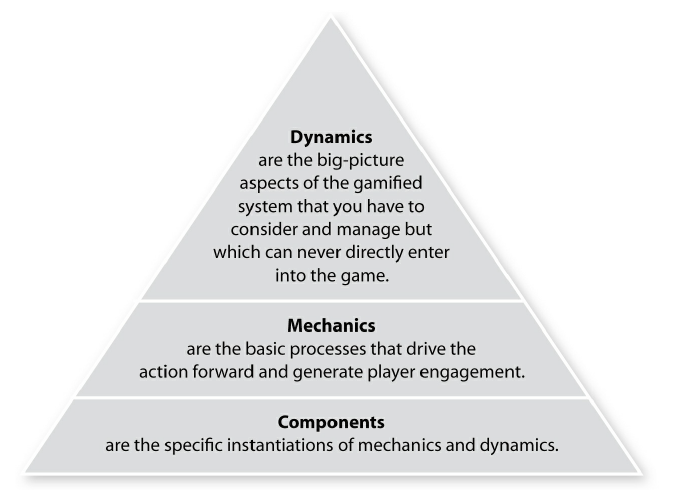
\includegraphics[width=0.75\textwidth]{mdc}
    \caption{The Pyramid of Game Elements from Werbach \& Hunter (2012, p. 82)}
    \label{fig:mdc}
\end{figure}
In the next section different mechanics, dynamics and components are listed and described according to their relevance and applicability to our context.
\subsubsection{Dynamics}
At the highest level of abstraction are game dynamics and serve as the core,  underlying framework for the Gamification to take place. Furthermore, they represent the implicit structure that guide the game, set  up  the  rules and constraints and  define the overall purpose, aim and goal of the game \cite{werbach2012win, WerbachCoursera}. 
According to Werbach and Hunter, the most important game dynamics are \cite{werbach2012win}:
\begin{itemize}
\item \textbf{Constraints}(limitations or forced trade-offs). Every game has some constraints, because games create meaningful choices and interesting problems by limiting people's freedom. So the notion of what constraints get put on users is an important dynamic that any game designer needs to think about. 
\item \textbf{Emotions}. Games can produce various emotions, from joy and sadness to everything in between. However, Werbach argues that the emotional palette of gamification is typically somewhat more limited \cite{WerbachCoursera}. The reason for this is because Gamification deals with real world, non-game context, such as marketing, or exercise context. In contexts like those, getting someone, for instance, really upset, will probable not be beneficial and valued. But there still are a variety of emotional levers that can be pulled, that can make the experience more rich, and certainly the joy, the, the sense of accomplishment, the emotional reinforcement that pushes people to play more, is important in most examples of gamification. 
\item \textbf{Narrative} (a consistent, ongoing storyline) Narrative: the structure that pulls together the pieces of the game, or the gamified system into some coherent feeling whole. The narrative can be explicit, the storyline in a game, or it can be implicit. And gamification doesn't necessarily have the richness of the aesthetic experiential aspect of games to put the work in creating a narrative. It has to rely upon things like consistent graphical experiences, creating a sense of flow and alluding to certain kinds of practices or certain kinds of story ideas that may be in players' heads using those, again, to tie together the individual pieces. If there's no sense of narrative, then the risk is that the gamified system will just be a bunch of abstract stuff. You get these badges. You get these points, but they're totally divorced from any sense of coherence and relation to the player's life and that tends to limit the effectiveness of gamification.
\item \textbf{Progression} (the player's growth and development)
\item \textbf{Relationships} (social interactions generating feelings of camaraderie, status, altruism, and so on)
\end{itemize}
\subsubsection{Mechanics}
Kevin Werbach describes game mechanics as ``the processes that drive actions forward''. He subsequently compared mechanics to ``verbs'' which help people to play games (see Fig. 2). In their academic article, Robert Hunicket et al. defined game mechanics as “the particular components of the game, at the level of data representation and algorithms”.

Mechanics are the basic processes that drive the action forward and generate player engagement. We
can identify ten important game mechanics:

\begin{itemize}
\item Challenges (puzzles or other tasks that require effort to solve)
\item Chance (elements of randomness)
\item Competition (one player or group wins, and the other loses . . . )
\item Cooperation (players must work together to achieve a shared goal)
\item Feedback (information about how the player is doing)
\item Resource Acquisition (obtaining useful or collectible items)
\item Rewards (benefits for some action or achievement)
\item Transactions (trading between players, directly or through intermediaries)
\item Turns (sequential participation by alternating players)
\item Win States (objectives that makes one player or group the winner—draw and loss states are
related concepts)
\end{itemize}
\subsubsection{Components}
Components make up the largest fraction of game elements. They can be viewed as more-specific forms that mechanics or dynamics can take. These elements are less abstract than the categories described previously and lead to tools that can be used in order to begin incorporating Gamification in the environment of interest. There many game elements that can be successfully used in gamified environments. However, some are more common than others, and some are more influential in shaping typical examples of gamification. Werbach and Hunter examined over 100 implementations of Gamification and claim that three elements always appear: \textit{points, badges}, and \textit{leaderboards}. They further point out how these elements are so common within Gamification that ``they are often described as though they are Gamification'', even though they are not \cite{werbach2012win}.  Hamari \textit{et al.} (2014), in their comprehensive survey of peer-reviewed empirical studies on gamification, also found that these three elements ``were clearly the most commonly found variants" in the large variety of elements tested \cite{hamari2014does}. The same elements were listed and described by Zichermann (2011), alongside \textit{levels}, \textit{challenges/quests}, \textit{onboarding}, and \textit{engagement loops} \cite{zichermann2011gamification}. In the next section, these three elements, commonly represented by the acronym \textit{PBL}, will be discussed.
\begin{enumerate}
\item \textbf{Points}\\*
Points represent a running numerical value which is given for any single action or combination of actions. In Gamification, they are mostly used to encourage people to do things by collecting them. The main assumption is that players will work harder in exchange for points. This is a very simple approach that occasionally works in motivateing those payer types who like collecting things or who like competing against each other. According to Zichermann and Cunningham (2011) points are ``an absolute requirement for all gamified systems'' and can serve a wide range of purposes, from obvious to barely visible ones. One of the most obvious usage of points and points systems is to for keeping a score. This way, points also provide a way of determining how well someone is doing in the game. So points can either show the relative position of players or they can actually define winning \cite{WerbachCoursera}. Werbach argues that points can also create a connection between progression in the game and extrinsic rewards since gamified systems offer some real-world prizes for reaching certain levels or number or virtual points. Another purpose for points is to provide feedback of the action. Explicit and frequent feedback represent a key element in most good game design, and points provide feedback quickly and easily and, by doing so, they show, in real time, how one is doing in the game. Finally, points provide data for the game designer since the points that users earn can easily be tracked and stored which allows the designer to analyze important metrics about the system. Zichermann and Cunningham (2011) distinguish five categories of point systems. According to the authors, points  can  be  divided  into  different categories  according  to  their  function. That is, one can differentiate among the following point systems: 
\begin{itemize}
\item Experience points,
\item Redeemable points,
\item Reputation points, 
\item Skill points, and
\item Karma  points
\end{itemize}
Each of the mentioned type of point system can have significantly different tasks in the gamified context. Even though, they can be a powerful motivator, Werbach and Hunter state that points are, in fact, very limited because of their uniform, abstract, interchangeable nature. That is, a point is only a point and nothing more. This is one of the reasons why badges are often found in conjunction with points systems.
\item \textbf{Badges}\\*
A badge represents a visual representation of some achievement within the gamified process \cite{WerbachCoursera, werbach2012win}. It should be noted that terms badges and achievements are often used interchangeably in
Gamification. They are a visual indication that a player has reached a certain level or accomplished some set of objectives \cite{werbach2012win, zichermann2011gamification}. When acquired, badges can serve a success indicator and, thus, possibly inspire players to achieve more badges. A well designed badge system, according to researchers Judd Antin and Elizabeth Churchill has five motivational characteristics \cite{werbach2012win}:
\begin{enumerate}
\item Badges can provide a goal for users exert oneself toward, which can positively affect players motivation
\item Badges can guidance as to what is possible and achievable within the system 
\item Badges are a signal of what a user cares about and capable of achieving. Thus, they are a visual marker of a player's reputation. That is the reason why players will often strive to acquire badges in order to show
others what they are capable of.
\item Badges can operate as virtual status symbols 
\item Badges can function as tribal markers. To put it more simple, a player who acquired some badges same as other players will feel a sense of identity and belonging with that group
\end{enumerate}
Werbach and Hunter point out that one of the most important attributes of badges is their \textit{flexibility}. That is, the possibilities with badge systems are immense and limited only by the imagination of the Gamification designer and the needs of the business. This allows the gamified system to target and suit the interest of a more diverse group of users in a way that is unachievable for a single point system \cite{werbach2012win}. 
\item \textbf{Leaderboards}\\*
The main purpose of a leaderboard is to make simple comparisons among players and to give context to progression in a way the points or badges usually can not. \cite{zichermann2011gamification, werbach2012win}. According to Werbach, in a context where performance matters, leaderboards can be very powerful motivators. That is, if a player sees that only few points are needed for moving up a slot or to emerge on top, it can be a strong motivator for pushing oneself harder in order to achieve that goal. However, in some situations leaderboard can be demotivating. In cases when the ranking lacks meaning or one notices how far behind the top ranked players is, a player can even decide to leave the gamified environment. According to Zichermann, there are various types of leaderboards used in gamified systems nowadays. However, the author encourages the usage of the \textit{no-disincentive leaderboard} in which, independent of the ranking order, the player is placed in the middle of the leaderboard where only the player's with a similar score can be seen. That way, one only sees how much is needed for the next best score, thus the possible demoivation by seeing how much is one behuind the top scored players is most probably avoided. A variant of this type of leaderboard, also used often in gamified systems, is the \textit{friend relative leaderbord} that only shows the score of people who are in the player's social graph. In this case, the player's score is compared not just to stranger but to people one is friends with \cite{WerbachCoursera}. Werbach, furthermore, points out that leaderboards do not need to track only one attribute, but it is up to the designer of to decide which attributes to be tracked. 
\end{enumerate}
The \textit{PBL triad} represents a useful starting point for building gamified solution, however, relying only on them can lead to negative outcomes \cite{werbach2012win}. This is because elements do not make the game \cite{werbach2012win, WerbachCoursera}. They are great tools for communicating progress and acknowledging effort, but neither points nor badges in any way constitute a game. This is where problems emanate. Heavily relying only on these elements, without understanding other aspects of game design could suppress players' intrinsic motivation, that is, their desire to engage with a game (or gamified service). However, no actual empirical evidence exists to back this claim \cite{mekler2013points}. Furthermore, when using the PBL triad, the most emphasis is put on rewards. The problem with this, according to Werbach, is that ``not all rewards are fun; not all fun is rewarding'' \cite{WerbachCoursera}. Thus, heavily relying only on rewards, might demotivate players in further engagement with the gamified system. On the other hand, Werbach claims that what can make elements successful is the ``way they are all tied together'', which often involves some higher level concepts such as dynamics. To sum up, even though PBLs have huge potential, they are not right for every project. That is why, some other elements should also be considered in order to ``extract the maximum value from Gamification''\cite{werbach2012win}. \\*
Apart from the described ones, there are other gamification mechanics that can be used, and these were identified by Werbach and Zichermann in their respective books. To 
In most games and gamified systems, levels indicate the players progress or they can serve as a marker reflecting the achievements and competence of the player in a gaming experience over time \cite{zichermann2011gamification}. Some of the most common are \cite{zichermann2011gamification, werbach2012win} 
\begin{itemize}
\item Achievements (defined objectives)
\item Avatars (visual representations of a player's character)
\item Collections (sets of items or badges to accumulate)
\item Combat (a defined battle, typically short-lived)
\item Content Unlocking (aspects available only when players reach objectives)
\item Gifting (opportunities to share resources with others)
\item Levels (defined steps in player progression)
\item Quests (predefined challenges with objectives and rewards)
\item Social Graphs (representation of players' social network within the game)
\item Teams (defined groups of players working together for a common goal)
\item Virtual Goods (game assets with perceived or real-money value)
\end{itemize}
According to Werbach the central task of a gamification design is putting all these elements together. However, one should keep in mind that no gamification system will and need to include all of these elements. On the other hand, it is necessary to take into account all the possible elements in order to build an engaging gamified service \cite{werbach2012win}. 

%just for health and fitness gamification
%First  the  elements  most related   to   motivation   are   presented   and   then   the   most   popular elements   in gamification  literature  are  presented.  Although  all  game  elements  can be  used  in gamification they might not all be equally relevant. Some are more potent and useful than others. As it is also a goal of this paper to examine which elements are the most  relevant,  based  on  the  research  done  on  motivational  theory  and  gamification literature a distinction is made.
%In theory, any context, task or process can be gamified \cite{muntean2011raising}. %skini i procitaj Muntean!! 

%\subsection{Objectives}
%\subsection{Principles}
%\subsection{The impact of Gamification}
%\subsubsection{Gamification in sports - Effects and Objectives}
%The main goal of gamification is to engage the users Gamification’s main goal is to rise the engagement of users by using game-like techniques such asscoreboards and personalized fast feedback (Flatla et al, 2011) making people feel more ownership and purpose when engaging with tasks (Pavlus, 2010).\cite{burke2016gamify}
%\subsection{Gamification critiques}

\subsubsection{Elements and Player Types}

\subsubsection{Gamification Design}

\subsection{Gamification of Health and Fitness}
Gamification in Health and Fitness has rapidly emerged over the past decade as a tool to promote health and wellness, as evidenced by the number of applications found in Apple App Store and Google Play Store containing at least some Gamification element. 

 %The best examples of gamification are in the Health and Fitness industry, where games encourage exercise by turning physical activity into a game and by delivering health interventions for bad habits cessation, like smoking, overeating or poor hydration, and medication adherence. Application of mobile and wearable devices have proven to be effective platforms for health and fitness games due to its wide adaptation, ease of use and continuous proximity to the users and patients. Since gamification can be applied to almost any business model, serious or not, for this thesis, we restrict our concern of gamification to the solving of serious issues. In particular, we are focused on gamification of education and behavior change related to the serious world issue of childhood obesity

%\chapter{Research Design}\label{chapter:survey_one}

The goal of this chapter is to document and describe the evaluation process of the Immotion warm up exergame in this thesis. The process is separated into three stages. In the first stage we assess the prototype of our gamified system and its elements. We evaluate through a survey which features of the gamified system are appreciated the most and which the least, and hence can be removed or improved. In the second stage, based on the feedback and reactions received from the respondents in the first stage, we complete the implementation of the second release of our gamified system. In the last stage, we pilot-test our gamified system in a local fitness center and evaluate it through a pilot-test study. In order to measure overall acceptance of our gamified solution for warm up, different methods have been used which will be described in the following sections.  The data is visualized using \textit{Tableau Desktop 10.3} software.

\section{First Evaluation}

The results from this evaluation should help to answer the overall research questions of this thesis:
\begin{enumerate}
\item \textit{Can exergames with gamification elements make warm up routines more enjoyable and, thus, motivate individuals to warm up more regularly before physically more demanding exercises?}
\item \textit{Can exergames with gamification elements be used as a interactive guidance for individuals who do not know how to perform warm up routines before physically more demanding exercises?}
\end{enumerate}

\section{Quantitative Methods}
To gain a first insight into acceptance of the Immotion warm up game we created an online survey. The survey was created using \textit{Google forms} and was accessible for two weeks from 16th to 30th of July 2017. The survey has been advertised via social networking services (\textit{Facebook} and \textit{LinkedIn}) and e-mail lists. No incentives were used to collect responds for this survey. Since our gamified system ought to be used before physically more demanding exercise (training) in gyms, fitness and sports centers, we targeted individuals who are physically active and engage in some sort of physical (sport) activity on a regular or semi-regular basis. The goal of this survey was to explore general work out and warm up habits of the respondents and their preferences and general acceptance of a gamified solution of a warm up routine. The questions in the survey were divided into three parts. First, the participants were asked a set of general questions regarding their age, gender and education level. Next, their training habits and warm up preferences were assessed. Lastly, participants were showed a video of the prototype version of the warm up game and asked questions related to the presented gamified warm up solution. 

\subsection{General Questions}
In the first part of the survey, the respondents are asked general questions about their gender, age and education level. Total number of n = 446 individuals participated in the survey, of which n = 204 (45.7\%) were female and n = 242 (54.3\%) male. The age of the respondents ranged from 17 to 58 with an average age of 30.16 years (SD = 6.49). The  following trend chart in \ref{fig:AgeTrend} shows the number of respondents grouped by their age.\\
\begin{figure}[h]
    \centering
    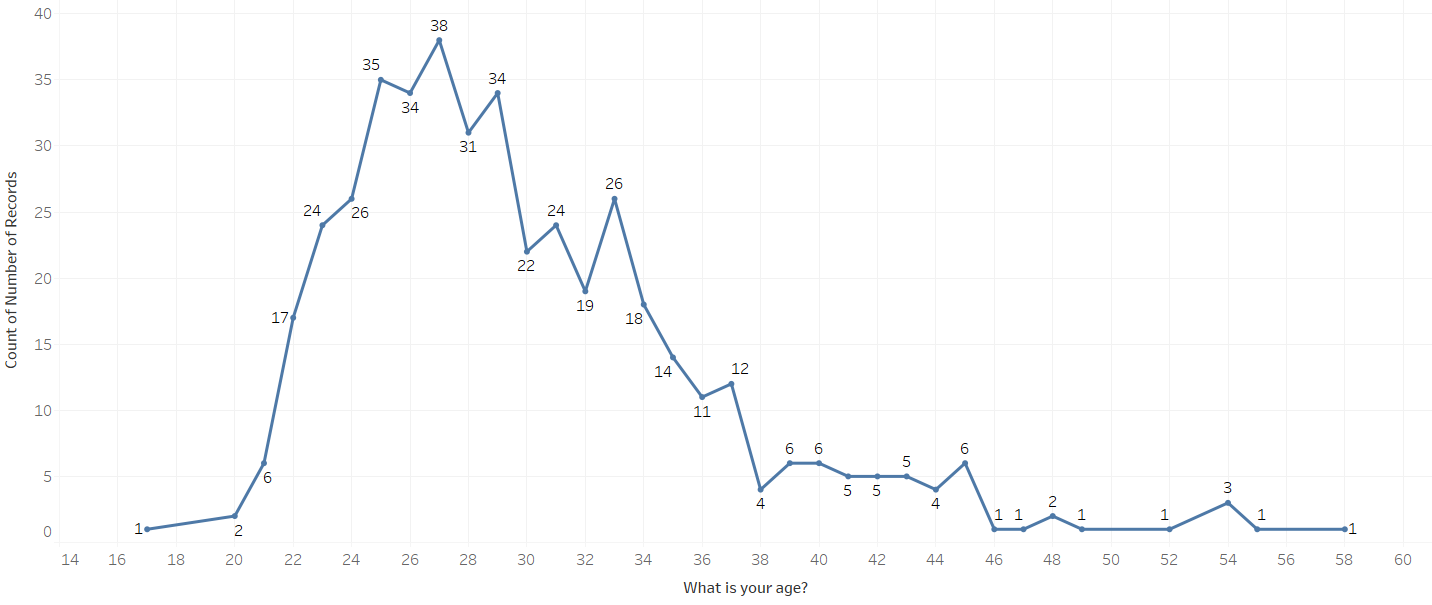
\includegraphics[width=\textwidth]{AgeTrend}
    \caption{The trend chart of respondents' age}
    \label{fig:AgeTrend}
\end{figure}\\
We observe that the most number of the survey participants are between 22 and 35 years old.\\
Regarding participants' education level, the majority of the respondents completed either their Master's studies n = 209 (46.9\%) or Bachelor studies n = 151 (33.9\%). The pie chart in \ref{fig:Education} shows the number of respondents based on their education level. 
\begin{figure}[h]
    \centering
    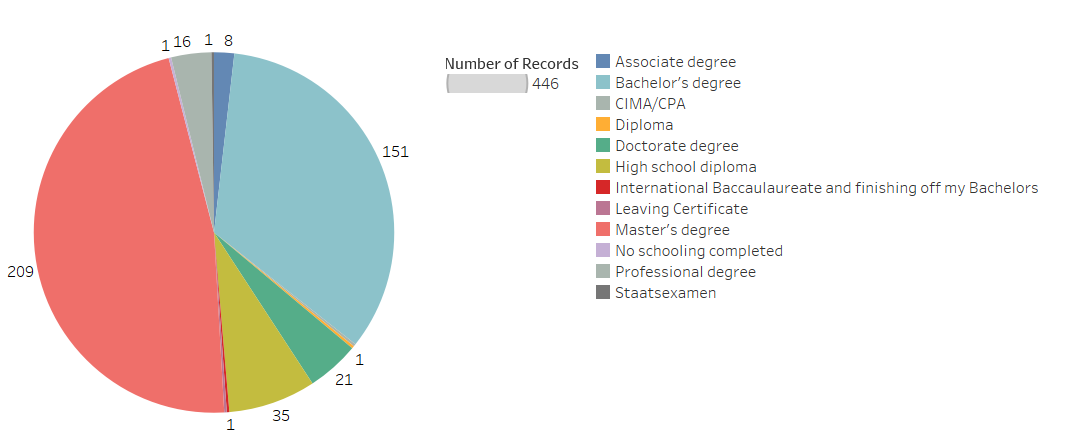
\includegraphics[width=\textwidth]{Education}
    \caption{Respondents' education level}
    \label{fig:Education}
\end{figure}
\subsection{Questions Related to Work Out and Warm Up Preferences}
The second section of the survey evaluated the respondents work out and warm up preferences. Total number of n = 442 of the respondents were amateur (recreational) athletes (99.1\%), while only n = 4 individuals declared themselves as being a professional athlete. In the survey, the respondents were pointed out that the most basic difference between amateur and professional athletes lies in the rewards that each group receives for athletic performances. Generally speaking, amateur athletes are not paid for their athletics performances. Professional athletes, by contrast, are typically paid annual salaries plus incentives tied to individual and team performance \cite{amateurvsproffesional}. More than half of the respondents (n = 357) reported taking part in some sort of sports activities during the whole year (77.4\%), while n = 101 (22.6\%) only few months per year. This means that most of the respondents engage in physical activities regularly without any longer stoppage.\\Regarding weekly training session occurrences, n = 152 respondents reported having 1 to 2 (34.1\%) and n = 168 having 3 to 4 (37.7\%) work out or sports sessions per week, while n = 54 (12.1\%) respondents reported taking part in sports activities irregularly (less than once per week). Most of the respondents (n = 285) reported having training sessions which last between 1 and 2 hours (63.9\%). The second most prominent training session duration reported by n = 125 respondents was less than an hour (28\%). Only n = 35 respondents reported having sport session with duration more than 3 hours. In \ref{fig:wuPreferences}, the pie chart on the left shows the percentage of respondents based on the number of training sessions per week. The pie chart on the right shows the percentage of respondents based on the duration of their training session. Moreover, n = 251 respondents stated that they prefer exercising alone (56.3\%), n = 86 (19.3\%) with a friend (or friends) and n = 109 in a group (24.4\%). Having a personal trainer was not prevalent among the respondents, and only n = 52 reported exercising with a personal trainer. 
\begin{figure}[h]
    \centering
    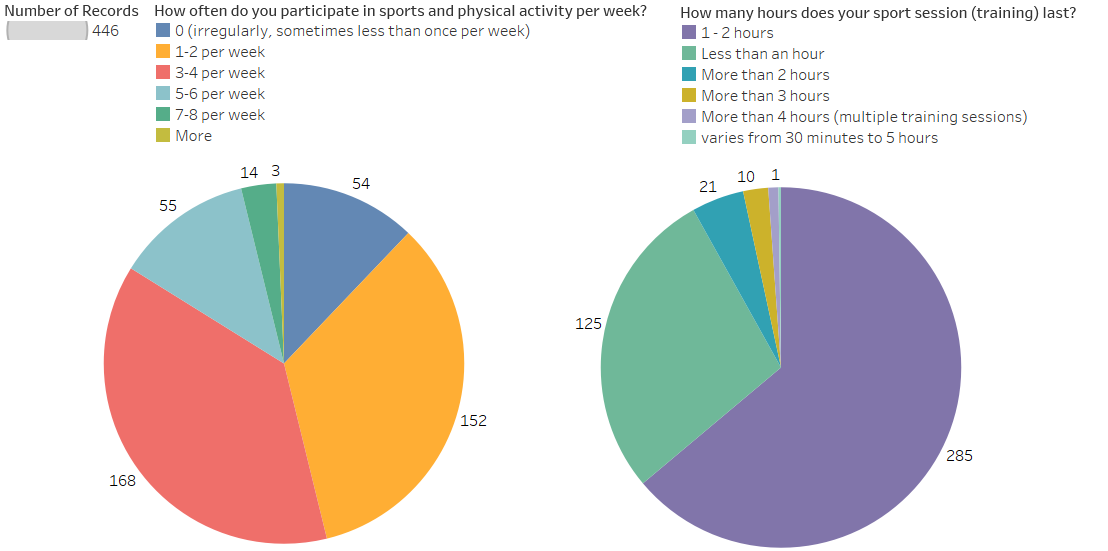
\includegraphics[width=0.80\textwidth]{wuPreferences}
    \caption{Respondents' weekly training session number and training duration}
    \label{fig:wuPreferences}
\end{figure}\\
When asked about their warm up preferences before a physical activity, n = 251 respondents (56.3\%) reported always warming up before physically more demanding exercises (or sports activities), whereas n = 195 (43.7\%) reported not warming up regularly before physically more demanding exercises (or sports activities). These results additionally confirm our assumption regarding absence of warm up habits in multitude of athletes. In \ref{fig:wuHabits}, we represent the respondents' warm up habits with regard their preferences to exercise alone, in a group or with a friend. 
\begin{figure}[h]
    \centering
    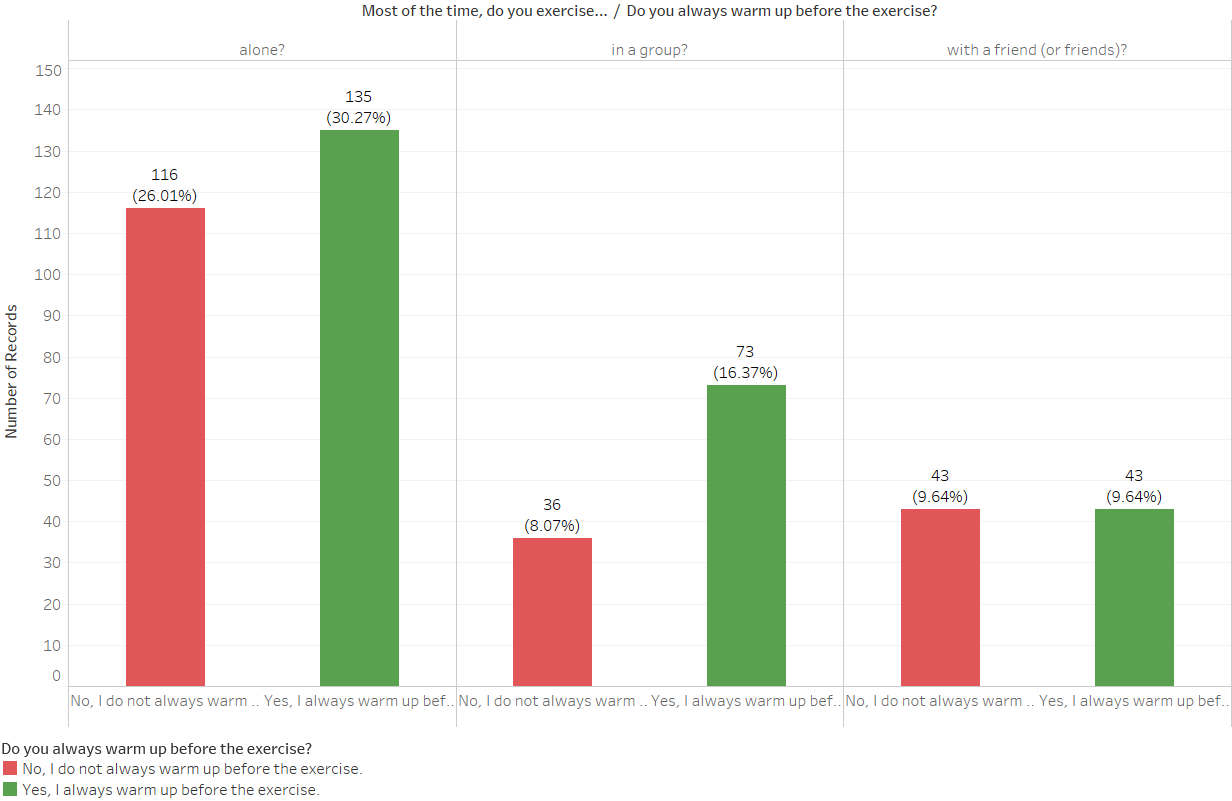
\includegraphics[width=0.80\textwidth]{wuHabits}
    \caption{Sum of Number of Records for the question ``\textit{Do you always warm up before the exercise?}'' broken down by ``\textit{Most of the time, do you exercise alone/with a friend/in a group?}'' Color shows details about ``\textit{Do you always warm up before the exercise?}''}
    \label{fig:wuHabits}
\end{figure}\\
It is interesting to notice that the most number of respondents who stated not warming up regularly, reported preferring exercise sessions that are carried out alone. On the other hand, we notice that most individuals who reported exercising in a group, regularly warm up before some sports activity. Based on their answer regarding warm up preferences, respondents were further asked different set of questions. Respondents that have stated not warming regularly, have been asked about reasons for not doing so. On the other hand, respondents who reported warming up regularly have been inquired about the duration and types of warm up exercises they usually engage in.
\subsection{Questions Related to Warm Up Routines}
The pie chart in \ref{fig:wuDuration} shows the number of respondents based on the duration of their warm up sessions before physically more demanding exercise. Only those respondents who reported warming up regularly were asked this question. Among n = 251 respondents that reported always warming up before the training session, the most common duration was between 5 and 10 minutes (43.4\%). Next, n = 66 (26.3\%) reported warming up less than 5 minutes, n = 64 respondents (25.5\%) between 5 and 10 minutes and, lastly n =11 (4.4\%) reported warming up more than 15 minutes. Only one respondent reported warming up less than a minute. The answers related to warm up duration gathered from respondents gave us valuable information about the most prevailing duration of warm up sessions. By knowing this, we can limit the duration of our warm up game to correspond to the periods outlined by the respondents through the survey.   
\begin{figure}[h]
    \centering
    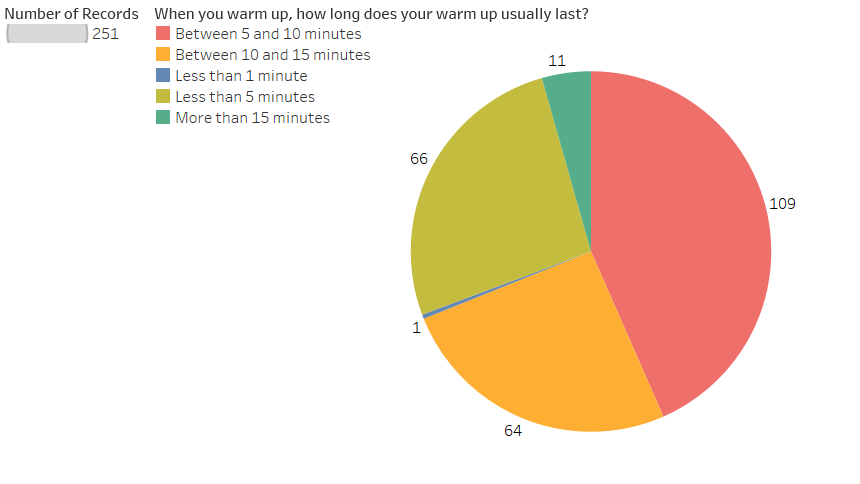
\includegraphics[width=0.90\textwidth]{wuDuration}
    \caption{ Responds to the question ``\textit{When you warm up, how long does your warm up usually last?}''}
    \label{fig:wuDuration}
\end{figure}\\
When the reported duration of the training session and warm up are compared among the respondents who stated warming up before the physically more demanding exercise, it is evident that the most common warm up duration is between 5 and 10 minutes regardless of the training session duration. In case of training sessions with duration less than 1 hour, the second most common warm up duration is the one that is less than 5 minutes long. On the other hand, in case of training sessions with duration between 1 and 2 hours, the second most common warm up duration is between 10 and 15 minutes. The highest number of respondents who stated warming up between 10 and 15 minutes belong to the group with the training session duration between 1 and 2 hours. In this group, less than 5 minutes warm up sessions were also customary. Overall, we can conclude that individuals do not tend to spend less than 1 and more than 15 minutes on the warming up procedure before physically more demanding exercises. The results are shown in \ref{fig:wuDuration2}.\\
\begin{figure}[h]
    \centering
    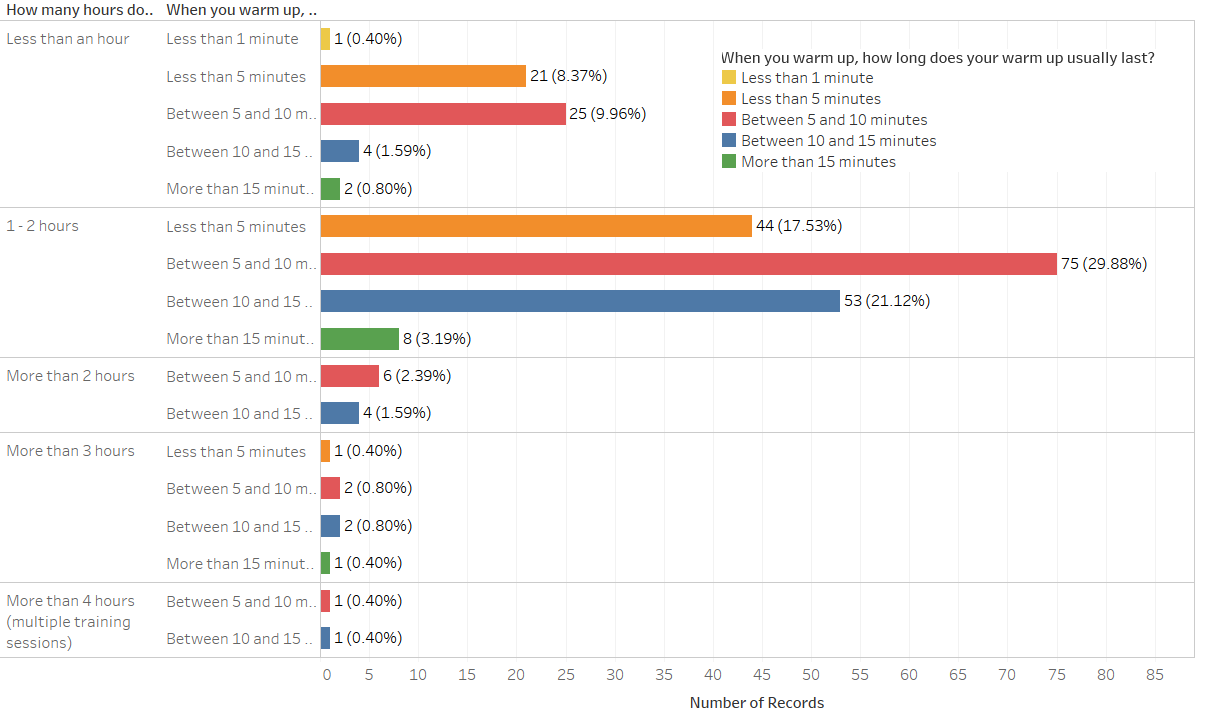
\includegraphics[width=\textwidth]{wuDuration2}
    \caption{Sum of Number of Records for each ``\textit{How many hours does your sport session (training) last?}''. Color shows details about ``\textit{When you warm up, how long does your warm up usually last?}''}
    \label{fig:wuDuration2}
\end{figure}\\
Taking this into account, the second release of the Immotion warm up game will enable players to choose the warm up duration they prefer the most. The available duration to choose from will be 1 minute, 2 minutes, 3 minutes, 5 minutes, 7 minutes, 10 minutes and 15 minutes which aligns to the duration pointed out by the respondents. These durations align also with the most common ones outlined in Chapter \ref{chapter:relatedwork} and suggested by different sources \cite{bishop2003warm2}.\\\\\\Respondents who reported warming up regularly were also inquired about the type of the warm up exercises they perform before the sport activity. Respondents could choose among three warm up types most often referred to in sports literature \cite{shellock1985warming, bishop2003warm2}, which were: 
\begin{itemize}
\item general warm up,
\item sport specific warm up (warm up that reflects the type of movements and actions which will be required during the sporting event), and 
\item passive warm up (e.g., taking a hot shower, having a rubdown, sitting in the sun)
\end{itemize} As mentioned, this question was asked only from those respondents that reported always warming up before the sport activity (n = 251). The most common warm up routine, reported by n = 140 respondents (55.8\%), was the sport specific type while the general (non-specific) warm up type was reported by n = 111 (44.2\%) of them. None of the respondents reported performing passive warm up before the more demanding physical activity. While using the Immotion warm up game, the player is asked to perform a set of general warm up exercises in order to complete the game. Hence, it was necessary investigate athletes preferences towards types of warm up routines they engage in most often. More than half of the respondents (55.8\%) reported engaging in sport specific warm up routine. This indicates that the respondents are more inclined towards specialized and personalized warm up routines, as opposed to the ones required in the prototype warm up game. Thus, the game should support players in selecting the set of warm up routines that are less general and more sport specific based on the sport they want to play (or group of muscles they want to warm up) or diversify and increase the types of movements the player needs to perform in order to successfully finish the game. %we believe that if the number and the type of movements are increased...%
Furthermore, n = 140 (55.8\%) respondents out of n = 251 reported having no inclination towards warming up in a group. Also, n = 101 (40.24\%) respondents stated not following any warm up procedure. Next, when asked about their preferences towards warming up when given instructions, n = 156 (61.4\%) out of n = 251 reported favoring warm up sessions when they are instructed and demonstrated by someone else. This is a valuable information because it suggests that individuals could, presumably, be inclined to warm up more regularly if they had a guidance through the warm up routine. With the Immotion game, we tackle exactly this requirement. By placing the obstacles that are to be avoided and coins to be collected, the athlete is instructed and guided through the warm up routine from the moment the game begins.\\The Immotion warm up game is designed and implemented as a single player game that guides the players through the warming up process and instructs them to perform specific movements in order to finish the game successfully and, consequently, warm up major muscle groups. Hence, it was required to assess these warm up preferences. In addition, out of n = 251 respondents, n = 111 (44.2\%) reported enjoying warm up sessions when they are carried out in a group. This leads us to believe that multiplayer (group) warm up should also be an option in the Immotion warm up game. That way, both athlete types (the ones preferring warming up individually and the ones not) can utilize and benefit from the game. Lastly, n = 150 respondents (59.76\%) stated following some warm up procedure. This result was unanticipated. However, it suggests that most of the athletes who took the survey and do warm up regularly, are well aware of the beneficial effects of warm up routines, and by following well established and accepted ones, are trying to maximize its positive outcomes. In \ref{fig:wuPrefPie}, the pie chart on the left shows the percentage of respondents who prefer warming up when given instructions (and those who do not), the pie chart in the middle shows the percentage of respondents who follow some recommended warm up procedure (and those who do not) in a group and those who do not and, lastly, the pie chart on the right shows the percentage of respondents who prefer warming up in a group (and those who do not).
\begin{figure}[h]
    \centering
    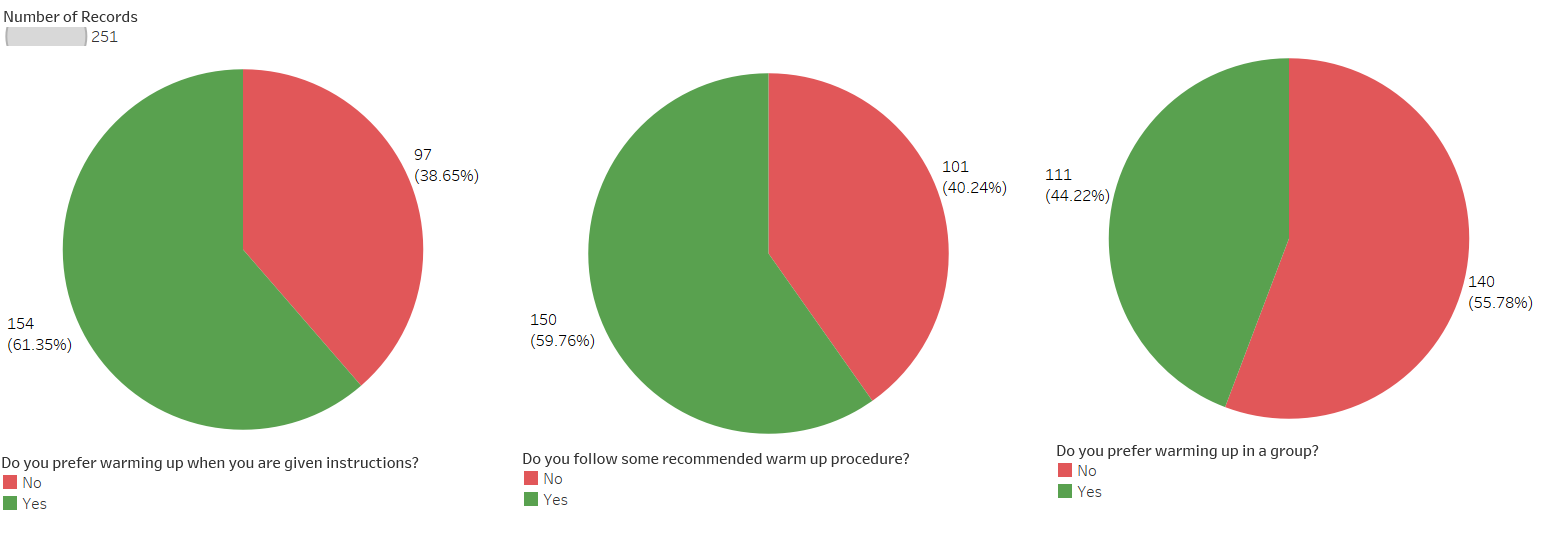
\includegraphics[width=\textwidth]{wuPrefPie}
    \caption{Respondents' answers for question ``\textit{Do you prefer warming up when you are given instructions}'', ``\textit{Do you follow some recommended warm up procedure}'', ``\textit{Do you prefer warming up in a group}''}
    \label{fig:wuPrefPie}
\end{figure}\\
The pie chart in \ref{fig:wuIntroduce} shows the number and percentage of respondents based on their answer on the question ``\textit{How were you introduced or recommended to the warm up procedure?}''.
\begin{figure}[h]
    \centering
    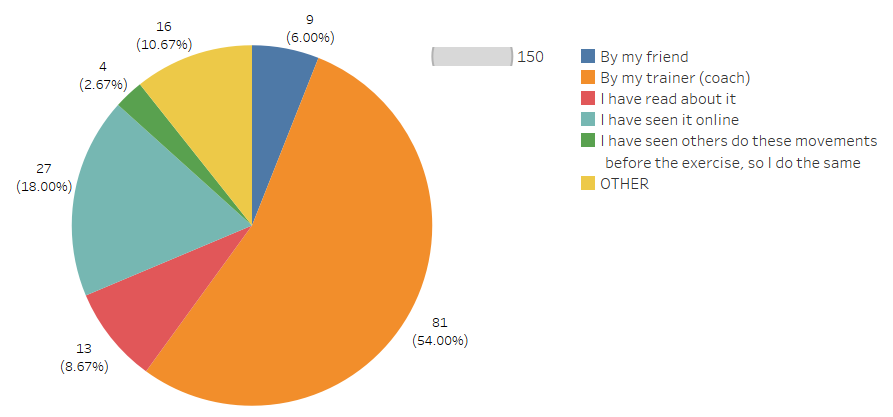
\includegraphics[width=\textwidth]{wuIntroduce}
    \caption{Sum of Number of Records and Percentage of Total Number of Records for the question ``\textit{How were you introduced or recommended to the warm up procedure?}''}
    \label{fig:wuIntroduce}
\end{figure}\\
Answering this question was optional, and it was asked only from those respondents who reported warming up regularly. Among n = 150 respondents that gave answer to this question, n = 81 (54\%) stated that they were introduced to the warm up procedure they perform by their coach, n = 27 (18\%) have seen the procedure online, while n = 13 (8.67\%) have read about it. The rest of the respondents reported seeing others do similar movements before the sports activity (n = 4) and to be introduced to the warm up procedure by their friend (n = 9). Some of the other sources, reported by n = 16 respondents were:
\begin{itemize}
\item ``\textit{I am a certified personal trainer, so I've adapted my learning to my own training}''
\item  ``\textit{Exercise APPs}''
\item  ``\textit{Physio + Personal trainers + coaches + YouTube channels}''
\item  ``\textit{Studied as part of college course}''
\end{itemize}
To assess respondents' attitude towards the importance of the warm up procedure before physically more demanding exercise, the respondents (n = 251) were asked to give their preferences regarding the following statements: 
\begin{itemize}
\item ``\textit{Warm up before exercise is important for me.}''
\item  ``\textit{Warm up before exercise can positively affect my performance.}''
\item  ``\textit{Warm up before exercise can reduce the likelihood of an injury.}''
\item  ``\textit{After my warm up routine, I feel I am prepared for the physically more demanding activity.}''
\end{itemize}
For each question, respondents could choose among five categories: \textit{Strongly Disagree}, \textit{Disagree}, \textit{Neutral}, \textit{Agree} and \textit{Strongly agree}. Each category is assigned a score from 1 (Strongly Disagree) to 5 (Strongly Agree). In \ref{fig:LS1} we show the  
\textit{Likert} scale score for the previous statements broken down by respondents' gender. For each question we assign a range of values that show how the survey responses are spread by category and a general feeling whether they are positive or negative. Based on the available categories and their total scores, we specify the dividing line and check how many responses are below and above it. That is, the dividing line is at 0\% and the responses left from it are generally negative, and right from it generally positive.  Each individual line shows a different starting point for each answer. The offset (lines' starting point) depends on the total number of negative scores, which are in our case the number of Neutral, Disagree and Strongly Disagree divided by the overall score for that question. The overall score (or the number of responses) for all the question is the same, since these questions were mandatory and all respondents answered it. Also, we split the Neutral answers and assign half of it to positive, and half to negative answers so we are not weighting unfairly one side to the other.  The width of each individual category depends on the number of records that are in that category over the total number of responses for the entire bar (that particular question). Lastly, we add the overall Likert scale score depicted as a yellow circle in each bar which shows the summary for each individual question.  
\begin{figure}[h]
    \centering
    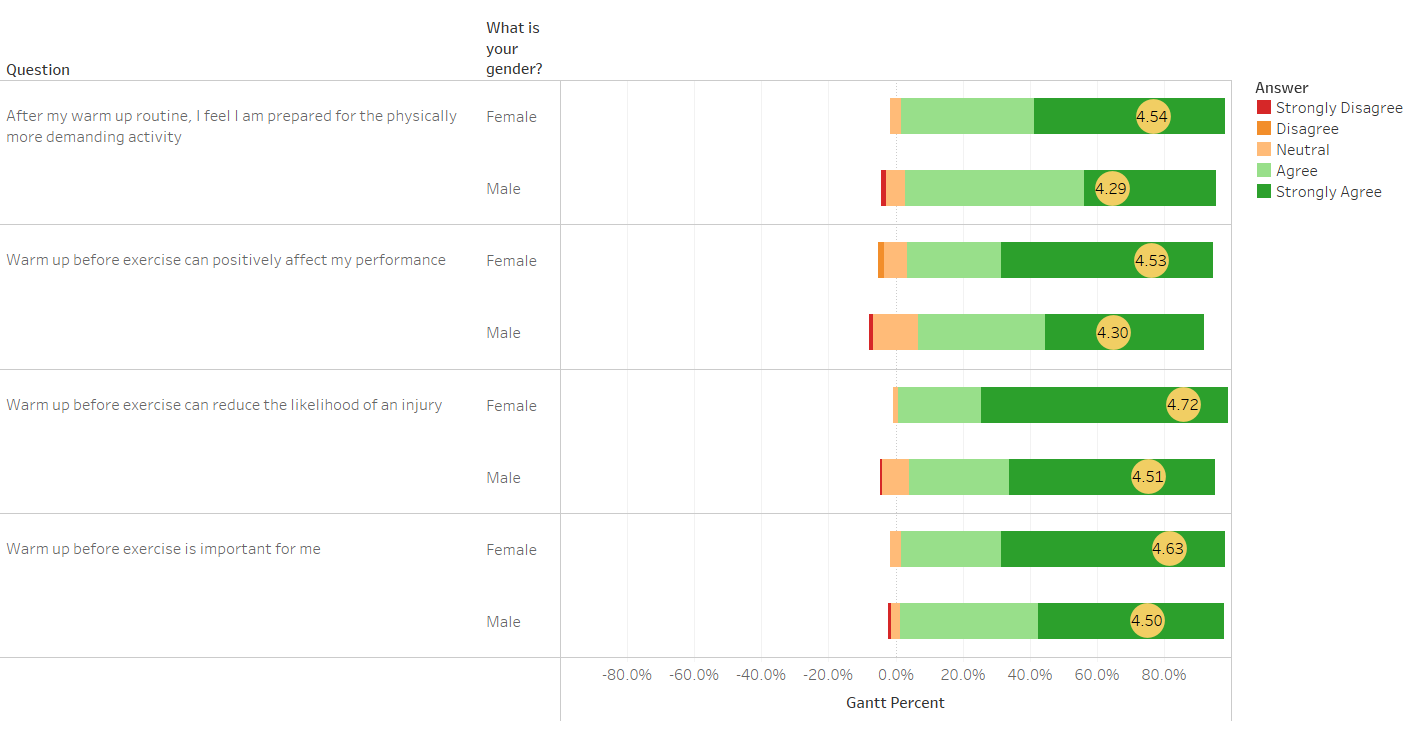
\includegraphics[width=\textwidth]{LS1}
    \caption{Gantt Percentage and the average score for the following statements: ``\textit{Warm up before exercise is important for me.}'', ``\textit{Warm up before exercise can positively affect my performance.}'', ``\textit{Warm up before exercise can reduce the likelihood of an injury.}'', ``\textit{After my warm up routine, I feel I am prepared for the physically more demanding activity broken down by respondents gender.}''}
    \label{fig:LS1}
\end{figure}\\
From the responses that are presented in \ref{fig:LS1}, we conclude that the respondents have a generally positive stand towards the statements given, since every question has an overall Likert score above 4 out of maximum 5. This positive bias was somewhat expected since the question was asked only from those who reported warming up regularly before sports activities. Some lower scores were obtained for male respondents in the first two statements ``\textit{After my warm up routine, I feel I am prepared for the physically more demanding activity}'' (4.29) and ``\textit{Warm up before exercise can positively affect my performance}'' (4.30) which might indicate that a number of the respondents, even though warming up regularly, do not perform the warm up procedure thoroughly and thus, do not feel fully prepared for the subsequent sports activity.\\ Respondents who stated warming up regularly were asked to describe their warm up routine or to list the most common exercises they perform in order to prepare for the physically more demanding ones. Since  n = 150 respondents (59.76\%) stated following some specific and well established warm up routines, we were interested in the most common movements and exercises these routines combine. Our primary goal was to use those movements and exercises in the game as movements for avoiding obstacles and collecting points. After the answers are collected, we group them based on textual occurrences of specific keywords and on textual occurrences of keywords with the same semantic meaning. The aggregated answers are shown in \ref{fig:5_describeWURoutine}.
\begin{figure}[h]
    \centering
    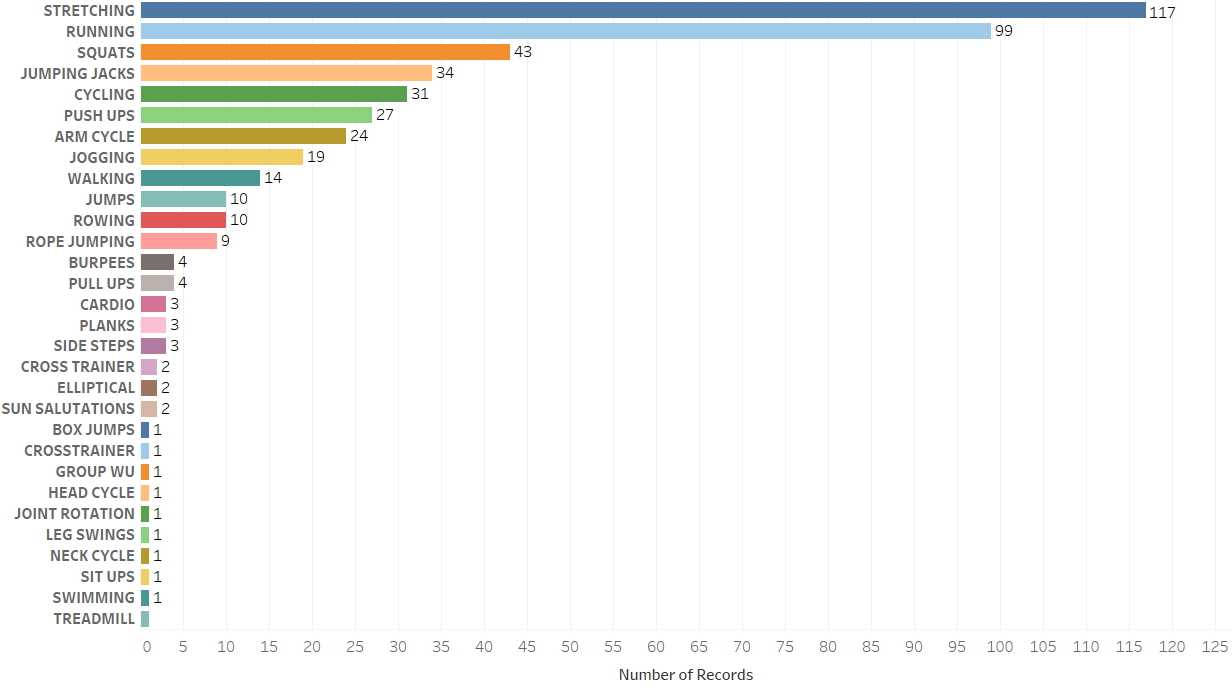
\includegraphics[width=\textwidth]{5_describeWURoutine}
    \caption{Summary of most common warm up exercises performed by the respondents}
    \label{fig:5_describeWURoutine}
\end{figure}\\
From \ref{fig:5_describeWURoutine}, we observe that the most of the respondents include stretching exercises in their warm up routine. This was expected since, when asked if they include stretching in their warm up procedure, out of n = 251 respondents, n = 205 reported performing, while n = 46 reported not performing stretching exercises during warm up session. We hypothesize that the reasons for this is that athletes confuse stretching with warming up and believe stretching exercises can prepare our body for strenuous activity as well as prevent injuries. However, as already pointed out in Chapter \ref{chapter:relatedwork}, there exists no scientific evidence for these assumptions. Additionally, in a recent study that included 2729 runners, static stretching had proved to have no effects in protecting against injury. According to the researchers, "stretching neither prevented nor induced injury when compared with not stretching before running" \cite{pereles2012large}. In some cases, a study published in Medicine and Science in Sports and Exercise (PubMed) found, it can even inhibit performance. After reviewing the available literature, the authors point out that static muscle stretches which are longer than 60 seconds are more likely to lead to a slight to moderate reduction in performance \cite{kay2012effect}. Hence, we believe that, by using our gamified solution, not only that athletes can prepare themselves for the subsequent physical exercises but also be more informed about the most efficient and practical movements that presumably reduce the likelihood for injuries and increase body performance for the subsequent physical activity. The second most common exercise is running (indoor and outdoor). The respondents usually start their warm up with a few minutes run after which they perform a full body stretching exercises. Apart from that, exercises like squats, jumping jacks, push-ups, arm cycles and cycling are also common exercises among the respondents. Some respondents, on the other hand, use treadmill, cross trainer, rowing and elliptical exercise machine for warming up. From the answers, we can conclude that respondents mostly focus on warming up their lower body parts in their warm up routines and in general finish the warm up routine with whole body stretching exercises. We also notice that most of the respondents do not follow any specific warm up routines and use general exercises before sports activities with strong focus on whole body stretching.\\Certain number of respondents, on the other hand, did not only list but described an exemplary warm up routine. Some of them are: 
\begin{itemize}
\item ``\textit{Warm up depends on exercise: e.g. warming up for heavy squats includes hip-opening exercises, core static exercises, mobility exercises for hip rotation/extension, low-weight squats.}''
\item ``\textit{For climbing: running on the spot, arm cycles, ankle rotations, active and passive stretches of leg, arm and back muscles.  For running: running on the spot, ankle rotations, active and passive stretches of leg muscles}''
\item ``\textit{I start with an activity to raise my heart rate and body temperature. Once that's accomplished, I work through stretching the major muscle groups first, then typically sit down to stretch out smaller/more specific muscle groups.}''
\end{itemize}
Based on these answers we introduce new movements for avoiding obstacles and collecting points in our second release of the warm up game. As for the respondents, our main focus are lower body parts. Even though it is expected by the respondents, stretching exercises will not be incorporated. However, we inform the athletes after the game ends about the most preferred stretching duration they can perform in order to maximize the subsequent performance and, possibly, avoid injuries. Since we are using only one Kinect device for gesture tracking, we avoid complicated movements that require prior exercise knowledge or experience and increased focus. Moreover, taking into account our hardware constraint, we choose movements that are easily detectable with only one Kinect sensor. 
\subsection{Reasons for Not Warming Up}
Respondents who reported not warming up regularly have been inquired about the reasons for not doing it.  Out of n = 195 respondents who reported not warming up regularly before sports activities, total of n = 321 responses have been collected, since some of the respondents gave multiple answers to this question. The most common reasons reported by the respondents were time constraint which was reported by n = 84 respondents and the monotonous and tiresome nature of the warm up procedure, reported by n = 81 respondents. Furthermore, n = 41 respondents pointed out that the reason for not warming up was because they do not know how to properly carry out the warm up procedure, while for n = 37 respondents stated that the warm up procedure represents an insignificant and negligible activity. Figure in \ref{fig:Reasons} shows the respondents' answers regarding reasons for skipping warm up exercises before physically more demanding exercises.
\begin{figure}[h]
    \centering
    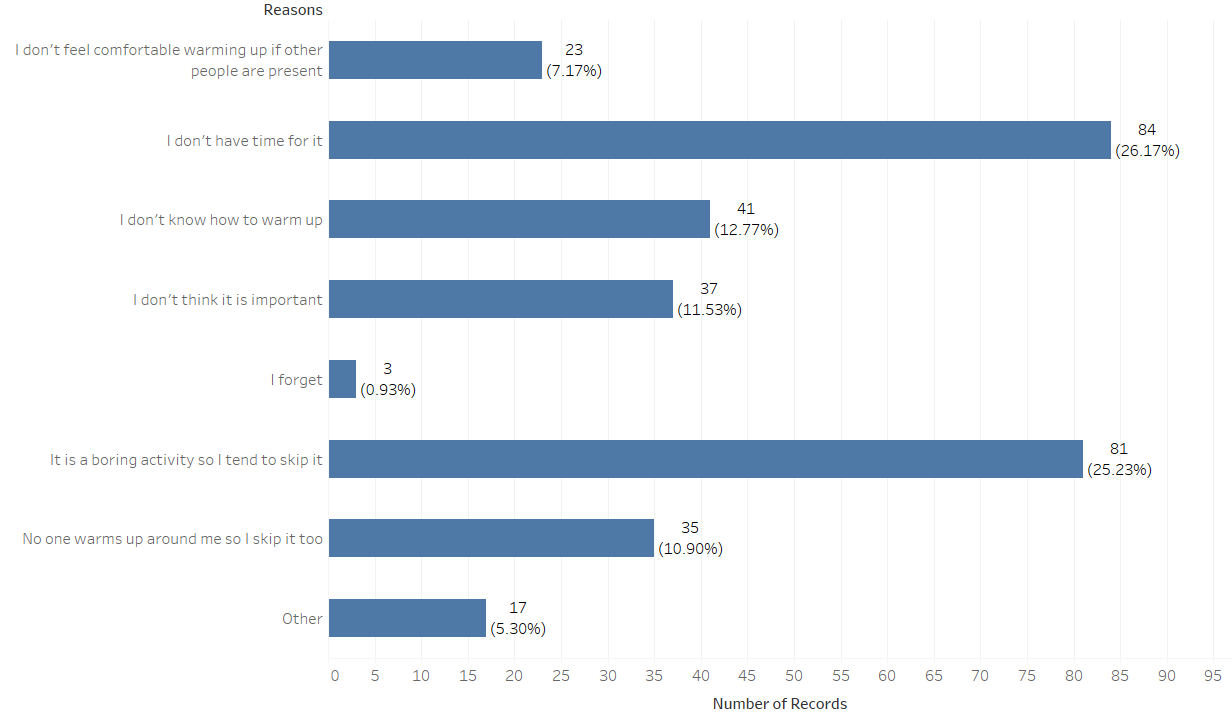
\includegraphics[width=\textwidth]{Reasons}
    \caption{Sum of Number of Records for respondents' reason for not warming up.}
    \label{fig:Reasons}
\end{figure}\\
Since this was an open ended question, a number of respondents left a comment regarding reasons for not warming up. We group all these answers in the Other category. Some of the other reasons for avoiding warming up pointed out by n = 17 respondents were: 
\begin{itemize}
\item ``\textit{I train climbing, so sometimes I can't wait to start climbing and skip the warm up.}''
 \item ``\textit{When I bike (for commuting) or do yoga, I don't warm up before, as I don't find it necessary.}''
\item ``\textit{I do a lot of endurance sports like running or biking. Warming up is kind of built in. If I do intervals, I do warm up.}''
\item ``\textit{It depends on the type of exercises - if I'm going for a bicycle ride I will skip warm up.}''
\item ``\textit{I feel it is better for me to warm up by playing the game.}''
\item ``\textit{It is part of the exercise. I dance, so the warm up is a dance routine.}''
\end{itemize}
We conclude that the reasons for not warming up are mostly tied to the specifics of the sports the respondents engage in. That is, these respondents believe that warm up for sports like biking, climbing or dancing are part of the exercise and they do not find it necessary to spend time for additional exercises that can prepare them for physically more demanding ones.\\In \ref{fig:ReasonsMaleFemale} we present the respondents' answers regarding reasons for skipping warm up exercises before physically more demanding exercises broken down by their gender.
\begin{figure}[h]
    \centering
    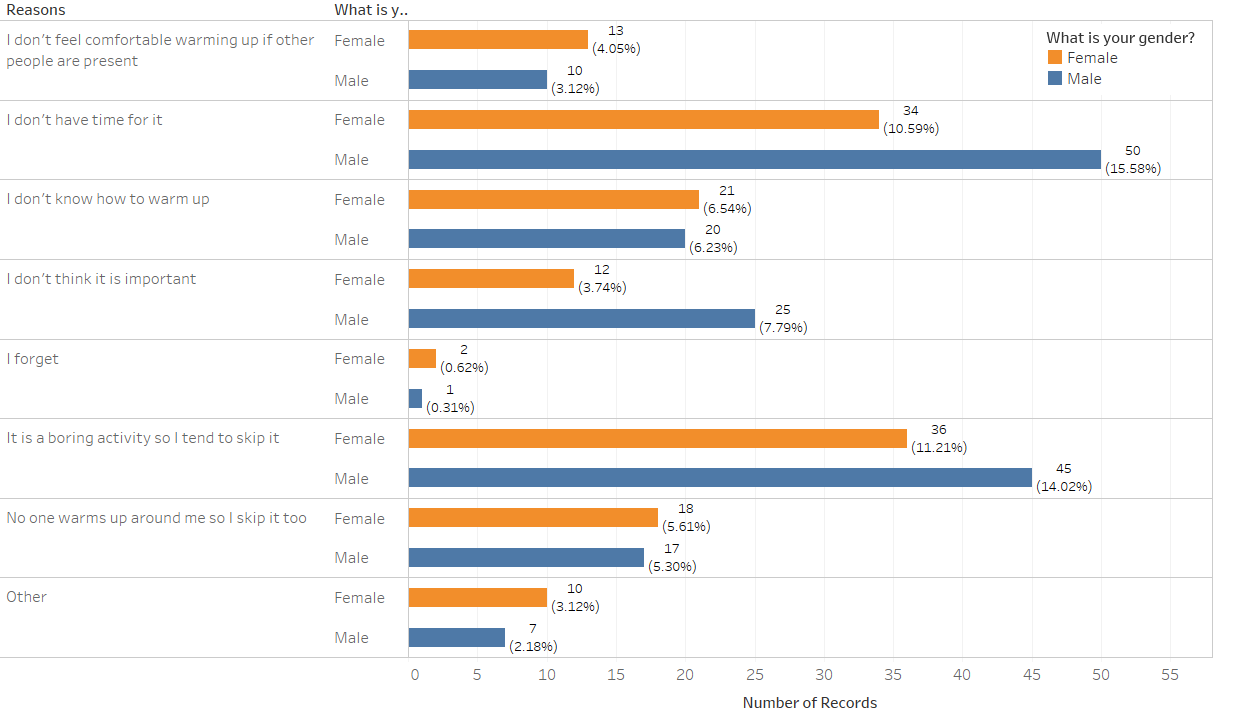
\includegraphics[width=\textwidth]{ReasonsMaleFemale}
    \caption{Sum of Number of Records for respondents' reasons for not warming up sliced by respondents' gender.}
    \label{fig:ReasonsMaleFemale}
\end{figure}\\
From the responses depicted in \ref{fig:ReasonsMaleFemale}, we observe that there were more male respondents that reported time constraints, dullness and meaningless of the warming up procedure as main reasons for not warming up before sports activities. On the other hand, more female respondents reported not feeling comfortable warming up when other people are present, not knowing how to perform the warm up procedure and avoiding warm up exercises because no one is doing it as main reasons for not warming up before sports activities. \\Next, in \ref{fig:ReasonsDoYouExercise} we present the respondents' answers regarding reasons for skipping warm up routine before physically more demanding exercise separated by their preferences toward warming up alone, with a friend or in a group. We notice that the most number of respondents who reported not warming up due to time constraints (n= 51), monotonous (n = 47) and, for them, meaningless nature (n = 25) of the warm up procedure usually engage in sports activities alone. 
\begin{figure}[h]
    \centering
    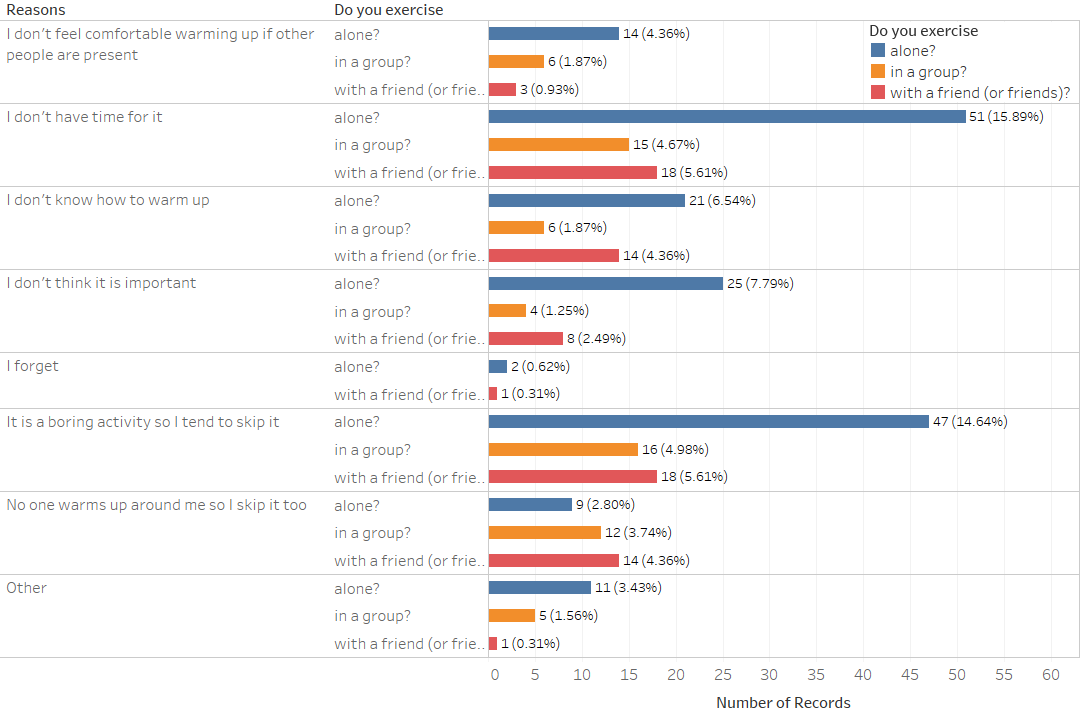
\includegraphics[width=\textwidth]{ReasonsDoYouExercise}
    \caption{Sum of Number of Records for respondents' reasons for not warming up sliced by respondents' work out preferences.}
    \label{fig:ReasonsDoYouExercise}
\end{figure}
Moreover, we observe that individuals tend to skip warm up more in cases when no one warms up in the group they are part of. That is, respondents who reported preferring sports activities which are carried out in a group or with a friend are likely to skip the warm up procedure if no one in the group engages in the warm up routine. In addition, this was the only case where a reason for not engaging in warm up had more responses in a category of respondents that usually work out with a friend or in a group. For all other reasons, most of the respondents belong to a category in which individuals reported engaging in sports activity usually alone. Hence, we conclude that individuals who carry out a sports activity alone, are more likely to skip the warm up routine than the ones doing it with a friend or in a group.\\ Overall, the results obtained in this question align with the ones acquired by Fradkin, \textit{et al.} (2010) in their survey on golfers and their warm up habits \cite{fradkin2010effects}. This further confirms the assumption addressed in this thesis and justifies the need for a solution that will motivate athletes to warm up more regularly before sports activities. Considering all the physiological and psychological benefits of a proper warm up routine and its suggested role in injury prevention covered in Chapter  \ref{chapter:relatedwork}, it is still perceived as a tiresome and meaningless activity and hence avoided by many amateur and professional athletes. Thus, educational and motivational solutions, that are enjoyable and easy to carry out, with primary focus on the major muscle groups and benefits of warm up need to be developed and implemented in order to increase the proportion of athletes who engage in warm up routines before every strenuous exercise.\\
With the Immotion warm up game, we tackle these issues brought up by the respondents. Making the game interactive and appealing, with intervals that last as long as the player chooses to, the warming up procedure undergoes a shift from a repetitive and tiresome activity to an entertaining and challenging necessity. Time constraints, mentioned by n = 34 female and n = 50 male respondents, will not be prevalent, since the player can choose the duration of the warm up session and by doing so plan ahead the work out session. These values are derived from the most common warm up duration reported by the respondents in \ref{fig:wuDuration}. Furthermore, athletes who do not know how to warm up and which movements to perform (mentioned by n = 21 female and n = 20 male respondents) in order to prepare their body for the subsequent sports activity, will be instructed through the game to perform a set a general warm up exercises. We believe that the guidance offered in our exergame could make the warm up routine more inviting for athletes who most often avoid or do not know how to perform the warm up routine properly. Moreover, we hypothesize that, if the athletes are provided with the opportunity to warm up using our gamified solution, which is tailored for a general warm up routine, will warm up more regularly. In addition, our solution could hypothetically leverage the duration of a warm up routine. To test these hypothesises, in this survey we assess and analyze the general acceptance of our prototype version of the gamified solution for warm up. Next, in Chapter (to be added), in order to gain a deeper insight into the findings from this survey, we conduct a user study in a fitness center with the second release of out gamified system.
\subsection{Questions Related to the Immotion Exergame}
In the last, third part, of the survey, the respondents were shown a short video with the prototype of the Immotion exergame. The short video showed how the warm game is used and the environment of the game, together with the obstacles one needs to avoid in order to successfully finish the game. The prototype of the game contained 7 different segments each consisting of various obstacles that, in order to be avoided, required from the user to perform a specific movement. The game lasted for 2 minutes and the movements the user of the game showed in the video had to perform in order to avoid the obstacles included: 
\begin{itemize}
\item jump right,
\item jump left,
\item jump up, and
\item squat.
\end{itemize}
After the video, the respondents were asked a set questions related to the warm up game in order to evaluate the general acceptance of the presented gamified solution for warm up.\\\\\\\\\\ Firstly, the respondents were asked if they would use the game for warming up before physically more demanding exercise. \\
\begin{figure}[h]
    \centering
    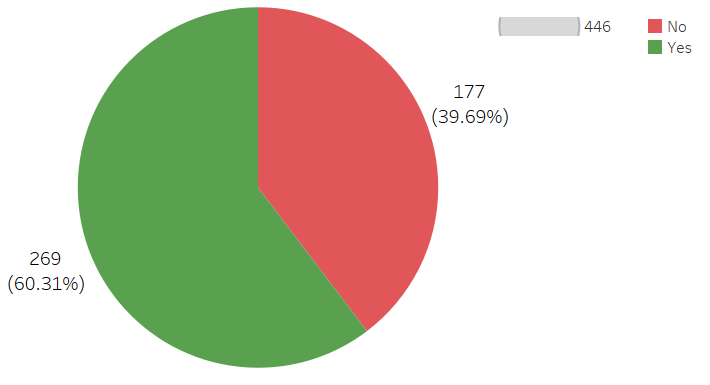
\includegraphics[width=0.8\textwidth]{immotionUsage}
    \caption{The Sum of Number of Records and Percentage of Total Number of Records for question ``\textit{Would you use the Immotion game for warm up?}''}
    \label{fig:immotionUsage}
\end{figure}\\
The pie chart in \ref{fig:immotionUsage} shows the number and percentage of respondents that would use the prototype game for warming up, and the number and percentage of the respondents who would not use the prototype game for warming up. From the information shown in this pie chart the green area resembles those who would use the Immotion game for warming up n = 269 (60.31\%) while the red resembles those who would not use it n = 177 (39.69\%). This question was asked from all the respondents (n = 446) regardless of their warm up preferences. From \ref{fig:immotionUsage} we conclude that the general acceptance of our gamified system is positive.\\ If we assess the respondents age compared to the Immotion game usage, we observe that the game is generally accepted by the respondents between age 22 and 37 years old. Negative responses concerning the warm up game usage are received from the respondents who were older than 38 years, presented in \ref{fig:UsageAge}.\\
Next, the acceptance of the Immotion warm up game regarding respondents' preferences towards warm up before a physical activity is depicted in \ref{fig:usage}. Out of n = 195 respondents who reported not warming up before sports activities n = 124 (63.58\%) would use the Immotion game for warming up. On the other hand, out of n = 251 respondents who reported always warming up before sports activities, n = 145 (57.76\%) would use the Immotion game for warming up.We observe that the general acceptance of the game is relatively high in both categories of respondents. However, respondents falling into category of athletes who do not warm up regularly gave more positive answers compared to the athletes who warm up regularly. This might imply that our gamified system is more appealing to respondents who do not engage in warm up routines often, and hence, could motivate them to warm up more regularly, or at least, more than they do currently. Also, high acceptance of the warm up game in the category of athletes who warm up regularly also tells us that those athletes, even though reported having well established warm up routines, would possibly switch to our solution if they are presented with the option to do so.\\
\begin{figure}[h]
    \centering
    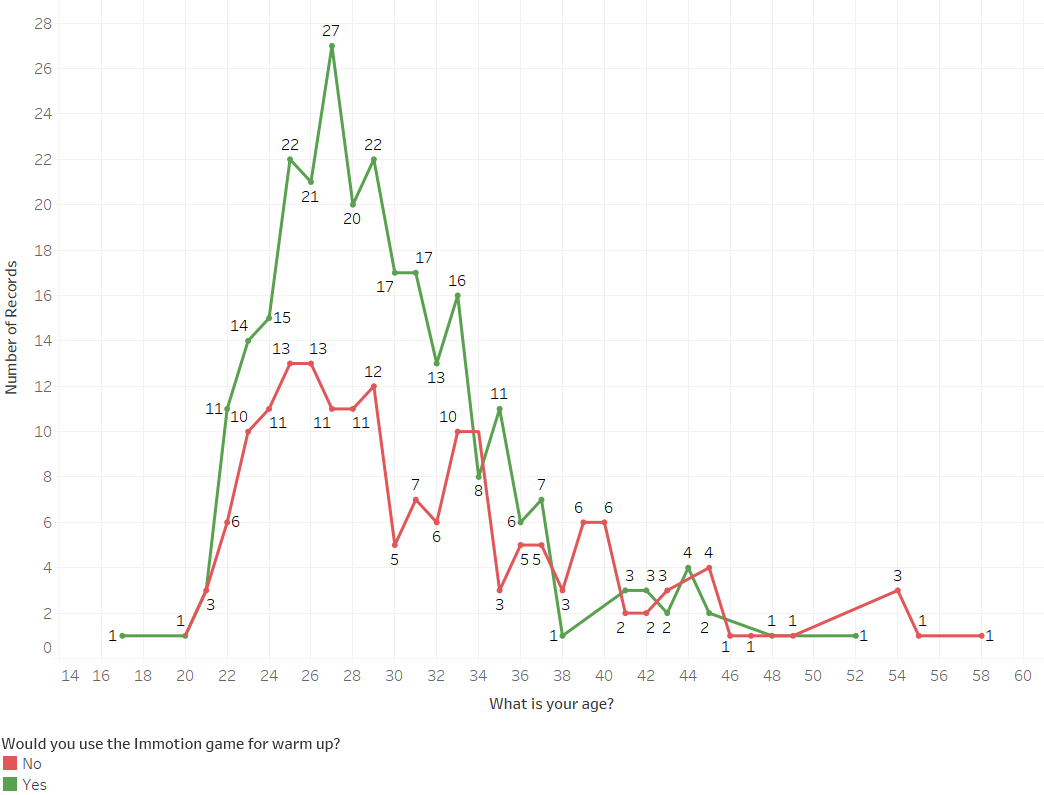
\includegraphics[width=0.8\textwidth]{UsageAge}
    \caption{The trend of sum of Number of Records for question ``\textit{What is your age?}''. Color shows details about responses to the question ``\textit{Would you use the Immotion game for warm up?}''}
    \label{fig:UsageAge}
\end{figure}
\begin{figure}[h]
    \centering
    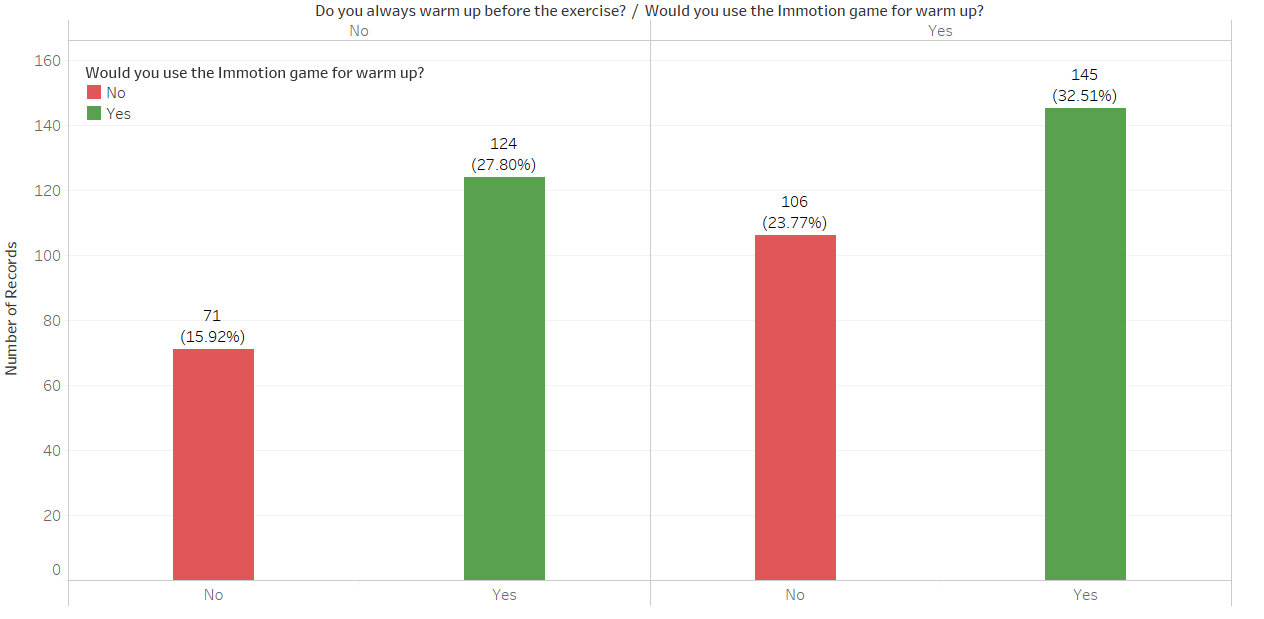
\includegraphics[width=0.9\textwidth]{usage}
    \caption{Sum of Number of Records for the question ``\textit{Would you use the Immotion game for warm up?}'' broken down by responses for question ``\textit{Do you always warm up before the exercise?}''. Color shows details about question ``\textit{Would you use the Immotion game for warm up?}''}
    \label{fig:usage}
\end{figure}\\
Since the player of the Immotion game is instructed when and what sort of movements to preform, we were interested in acceptance of the game among those respondents who prefer and do not prefer warming up when given instructions, shown in \ref{fig:warmupusage}.
\begin{figure}[h]
    \centering
    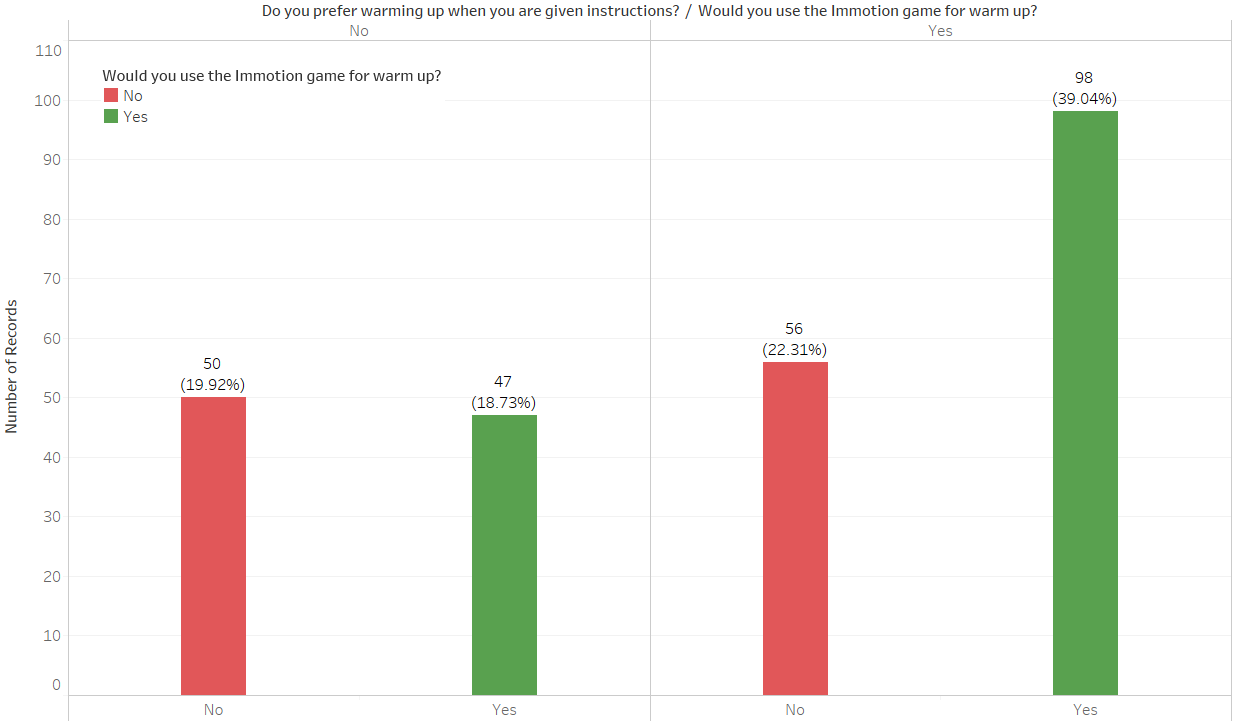
\includegraphics[width=\textwidth]{warmupusage}
    \caption{Sum of Number of Records for the question ``\textit{Would you use the Immotion game for warm up?}'' broken down by responses for the question ``\textit{Do you prefer warming up when you are given instructions?}''. Color shows details about the question ``\textit{Would you use the Immotion game for warm up?. }''}
    \label{fig:warmupusage}
\end{figure}\\
Out of n = 251 respondents who reported warming up regularly before sports activity, n = 97 stated not preferring having given instruction during the warm up exercises and n = 144 respondents stated that they prefer warming up when given instruction. From figure in \ref{fig:warmupusage}, we observe that out of all the respondents who do not like warming up when given insrtuctions, n = 50 respondents stated that they would not use the Immotion warm up game, while n = 47 respondents stated that they would use it. Contrarily, among respondents who prefer having instructions during warm up exercises, n = 56 stated that they would not use the warm up game, while n = 98 respondents reported that they would use it. From these responses, we see that the acceptance of the warm up game is much higher among those respondents who prefer warming up when given instruction and conclude that our gamified solution is more appealing for individuals who prefer warming up when given instructions. This also suggests that the warm up guidance and instructions that aree offered by our solution, could hypothetically influence individuals to engage in warm up routines more regularly.\\ Lastly, we analyze the warm up game acceptance broken down by respondents' preferences toward warming up alone, with a friend or in a group.\\\\
In \ref{fig:wuAloneUsage}, the respondents' answers are first sliced into categories based on the fact that they do or do not warm up before sports activities, and then broken down in subcategories based on their preferences toward warming up alone, with a friend or in a group.
\begin{figure}[h]
    \centering
    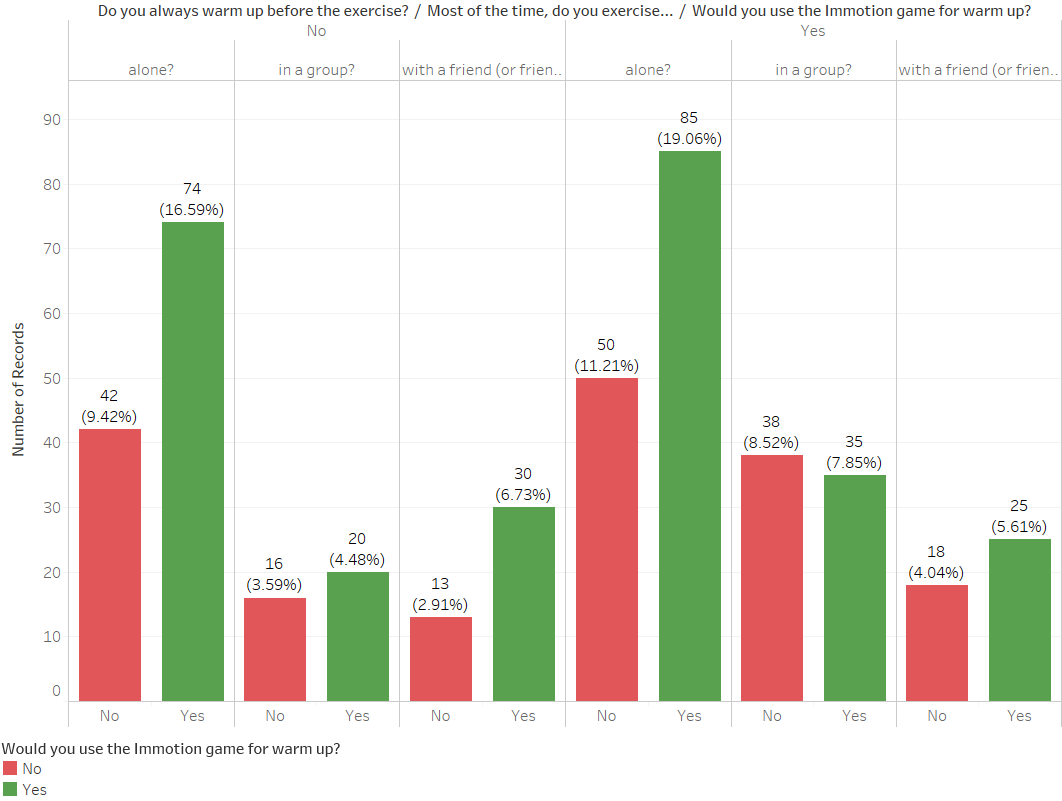
\includegraphics[width=0.75\textwidth]{wuAloneUsage}
    \caption{Sum of Number of Records for respondents' answers to ``\textit{Would you use the Immotion game for warm up?}'' broken down answers to ``\textit{Do you always warm up before the exercise?}'' and ``\textit{Most of the time, do you exercise alone, in a group or with a friend}''. Color shows details about answers to ``\textit{Would you use the Immotion game for warm up?}''}
    \label{fig:wuAloneUsage}
\end{figure}\\
We observe that the general acceptance of the warm up game is high in each subcategory (alone, with a friend, in a group) of respondents. The highest acceptance is among those athletes who prefer exercising alone (regardless of they warm up or not). The only subcategory where the disapproval of the gamified approach was higher than its acceptance, was among those respondents who warm up regularly and prefer exercises that are carried out in a group. We believe that the reason for this is the fact that the Immotion game, as shown in the video to the respondents, is a single player game which instructs the player to perform a set of general warm up movements. Respondents who engage in group (team) sports might not feel useful to spend time on general warm up exercises if the sport they engage in require specific movements. Furthermore, in exercises that are carried out in a group, it might not be time efficient to wait for every team member to complete the warm up routine using the proposed warm up game. That is, the proposed solution is not practical for the use case where athletes engage in group sports or exercises. This information, nevertheless, suggests that the target group for the Immotion warm up game should be individuals who prefer exercising alone or with a friend regardless if they warm up before sports activities or not.\\\\\\If we compare respondents' reasons for not warming up with respondents' general acceptance of the Immotion warm up game showed in figure \ref{fig:ReasonsWouldUse}, we observe that the game is generally accepted positively among all the respondents regardless the reasons they pointed out for not warming up.
\begin{figure}[h]
    \centering
    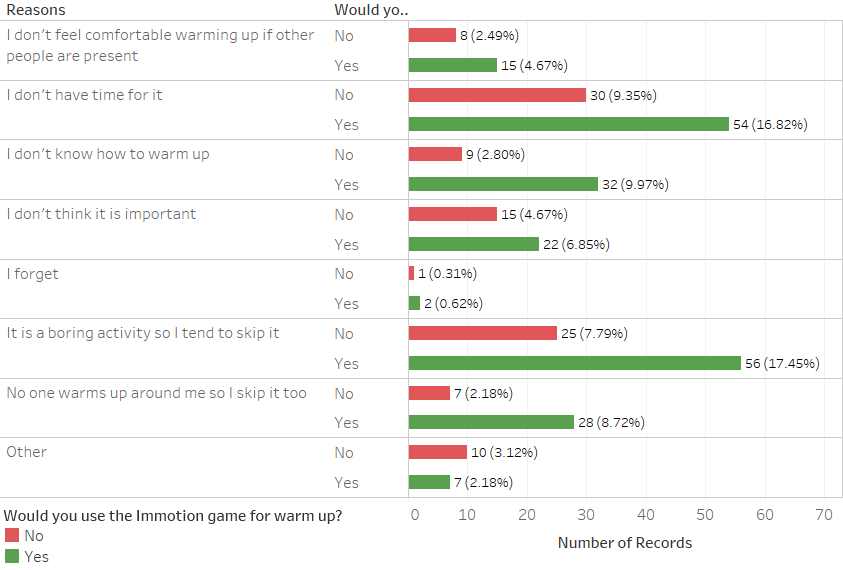
\includegraphics[width=0.9\textwidth]{ReasonsWouldUse}
    \caption{Sum of Number of Records for question ``\textit{Would you use the Immotion game for warm up?}'' broken down by respondents' reasons for not warming up. Color shows details about respondents' answers to the question ``\textit{Would you use the Immotion game for warm up?}''}
    \label{fig:ReasonsWouldUse}
\end{figure}\\
Lastly, when we slice the results based on respondents' gender, showed in \ref{fig:ReasonsWouldUseMakeFemale} , the result are similar to those depicted in \ref{fig:ReasonsWouldUse}. Overall, our gamified solution is positively accepted among all categories of respondents.\\ 
\begin{figure}[h]
    \centering
    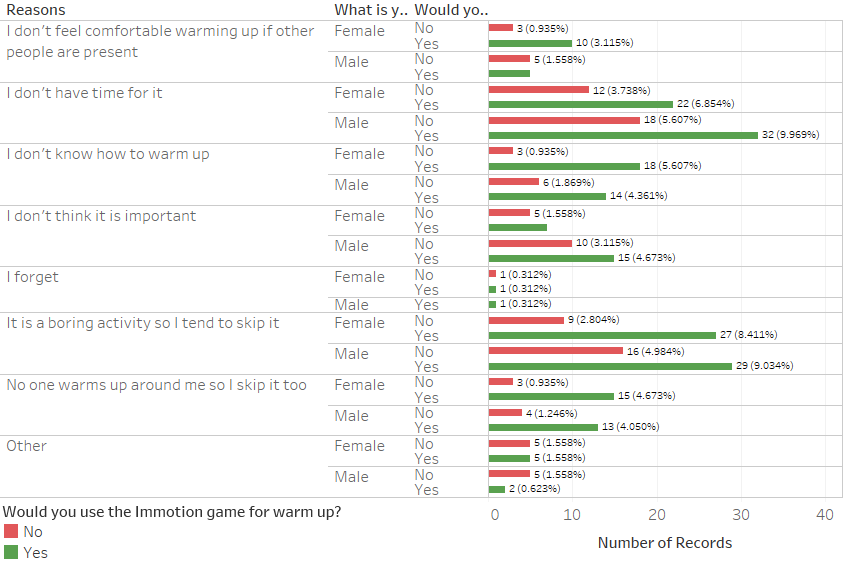
\includegraphics[width=\textwidth]{ReasonsWouldUseMakeFemale}
    \caption{Sum of Number of Records for question ``\textit{Would you use the Immotion game for warm up?}'' broken down by respondents' reasons for not warming up and respondents' gender. Color shows details about ``\textit{Would you use the Immotion game for warm up?}''}
    \label{fig:ReasonsWouldUseMakeFemale}
\end{figure}\\
To assess respondents' attitude towards the Immotion warm up game showed in the video, the respondents (n = 446) were asked to give their preferences regarding the following statements:
\begin{itemize}
\item ``\textit{I would rather use standard warm up routines instead of gamified warm up.}''
\item ``\textit{This approach (showed in the video) can increase the duration of my warm ups.}''
\item ``\textit{This approach (showed in the video) can increase the quality of my warm ups.}''
\item ``\textit{This approach (showed in the video) can make warm up more enjoyable for me.}''
\item ``\textit{This approach (showed in the video) can never work in practice for me.}''
\item ``\textit{This approach (showed in the video) could motivate me to warm up more regularly.}''
\end{itemize}
For each question, respondents could choose among five categories: Strongly Disagree, Disagree, Neutral, Agree and Strongly agree. Each category is assigned a score from 1 (Strongly Disagree) to 5 (Strongly Agree). Figure in \ref{fig:LS2} shows the Likert scale score for the previous statements sliced by respondents' preferences towards warming up before sports activities.\\
As in Likert scale presented in figure \ref{fig:LS1}, for each question we assign a range of values that show how the survey responses are spread by available categories and a general feeling whether they are positive or negative. Based on the available categories and their total scores, we specify the dividing line and check how many responses are below and above it. Each individual line shows a different starting point for each answer. The overall score (or the number of responses) for all the question is the same, since these questions were mandatory and all respondents answered it (n = 446). The width of each individual category depends on the number of records that are in that category over the total number of responses for the entire bar (that particular question). Lastly, we add the overall Likert scale score (LSS) depicted as a white circle in each bar which shows the summary for each individual question.  
From \ref{fig:LS2}, we observe that respondents who reported warming up regularly would rather use standard warm up routines instead gamified warm up solutions, like the presented Immotion warm up game (LSS = 3.59). On the other hand, respondents who do not warm up regularly mostly disagreed with the statements (``\textit{I would rather use standard warm up routines instead of gamified warm up.}'') or gave a neutral answer (LSS = 2.95). To be precise, n = 15 respondents strongly disagreed, n = 53 disagreed and n = 70 gave neutral answer out of n = 195 who reported not warming up before sports activity.\\ 
\begin{figure}[h]
    \centering
    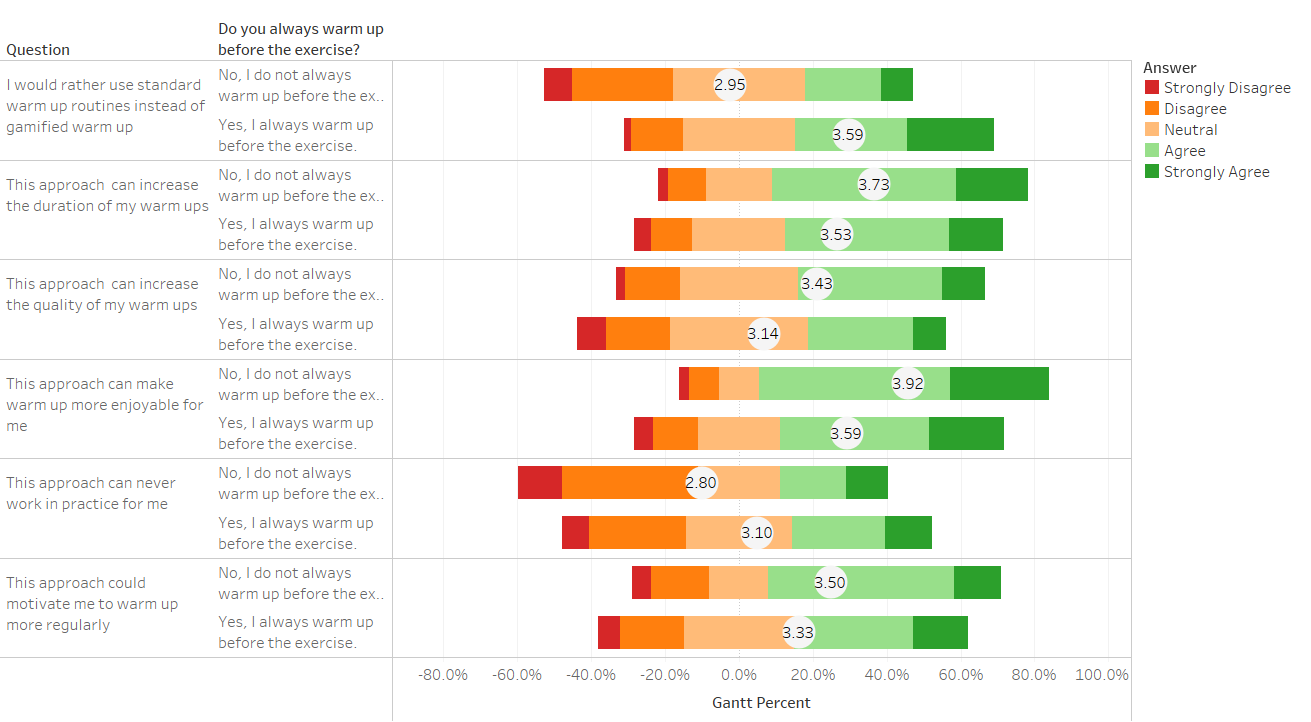
\includegraphics[width=\textwidth]{LS2}
    \caption{Gantt Percentage and the average score for question ``\textit{Do you always warm up before the exercise?}'' broken down by statements regarding the Immotion warm up game.}
    \label{fig:LS2}
\end{figure}\\ 
This suggests that most respondents falling into this category would likely use our gamified solutions as part of their work out (sports) routines. Regarding the second (``\textit{This approach (showed in the video) can increase the duration of my warm ups.}'') , third (``\textit{This approach (showed in the video) can increase the quality of my warm ups.}'') and sixth (``\textit{This approach (showed in the video) could motivate me to warm up more regularly}'') statement, both categories of respondents gave generally positive answers. However, respondents who warm up regularly gave more neutral answers (n = 63, n = 94 and n = 75 out of n = 251) which indicates their uncertainty about the possible positive effects this gamified solutions can have on the duration and the quality of the warm up procedure.  Similarly, in the fourth statement (``\textit{This approach (showed in the video) can make warm up more enjoyable for me.}''), responses given by both category of respondents were generally positive (LSS = 3.92, LSS = 3.59). This was, also, the statement that had the highest acceptance among respondents who do not warm up regularly. Overall, the results suggest that both categories see the gamified approach as a way of making the warm up routine more enjoyable and satisfying. The fifth statement (``\textit{This approach (showed in the video) can never work in practice for me.}'') received lover score (i.e. negative answers) from all the respondents. This corresponds to the previous results and suggests that respondents would presumably include this approach in their exercise routine if presented with the option.\\\\
If we slice the results by respondents' preferences towards exercising alone, with a friend or in a group, we observe that the respondents in all categories generally think that this gamified solution can increase the quality and the duration of their warm up routines and further make it more enjoyable, presented in \ref{fig:LS3}.\\
\begin{figure}[h]
    \centering
    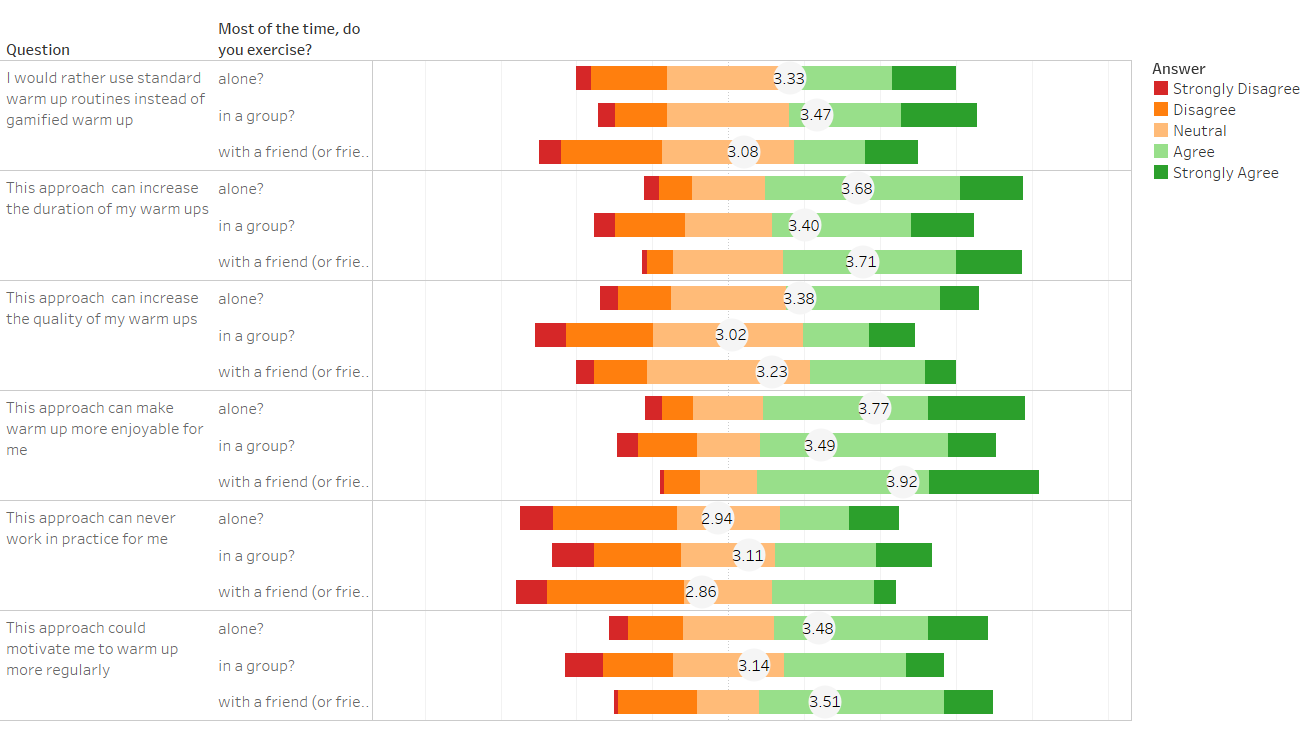
\includegraphics[width=\textwidth]{LS3}
    \caption{Gantt Percentage and the average score for question regarding respondents' preferences to warm up alone, in a group or with a friend broken down by statements regarding the Immotion warm up game.}
    \label{fig:LS3}
\end{figure}\\ 
Moreover, the possible positive affect that this approach can have on the consistency of the warm up sessions was received also well. The lowest scores were given by respondents who prefer exercises that are carried out in a group. In summary, taking into account the results depicted in \ref{fig:LS2} and \ref{fig:LS3}, our warm up game received positive acceptance from all the respondents, suggesting that it can hypothetically stand as a solution to increase the proportion of athletes who engage in warm up routines before every exercise or sports activity.\\ Lastly, all respondents were asked to leave their comments regarding the features they liked or disliked about the presented prototype warm up game, as well as to leave recommendations in case they have any. These questions were optional and not all the respondents actually responded. For all answered questions, we grouped the answers based on textual occurrences of specific keywords and on textual occurrences of keywords with the same semantic meaning.\\ In \ref{fig:1_mostImportantFeatures} we present the summary of responses regarding question ``\textit{What do you think are the most important features of this warm up game that would make you use it?}''\\\\ \\ \\
From \ref{fig:1_mostImportantFeatures} we observe that most of the respondents see the game as a fun, entertaining and enjoyable way for engaging in the warm up routine; a ``\textit{very new and creative idea to warm up}''.
\begin{figure}[h]
    \centering
    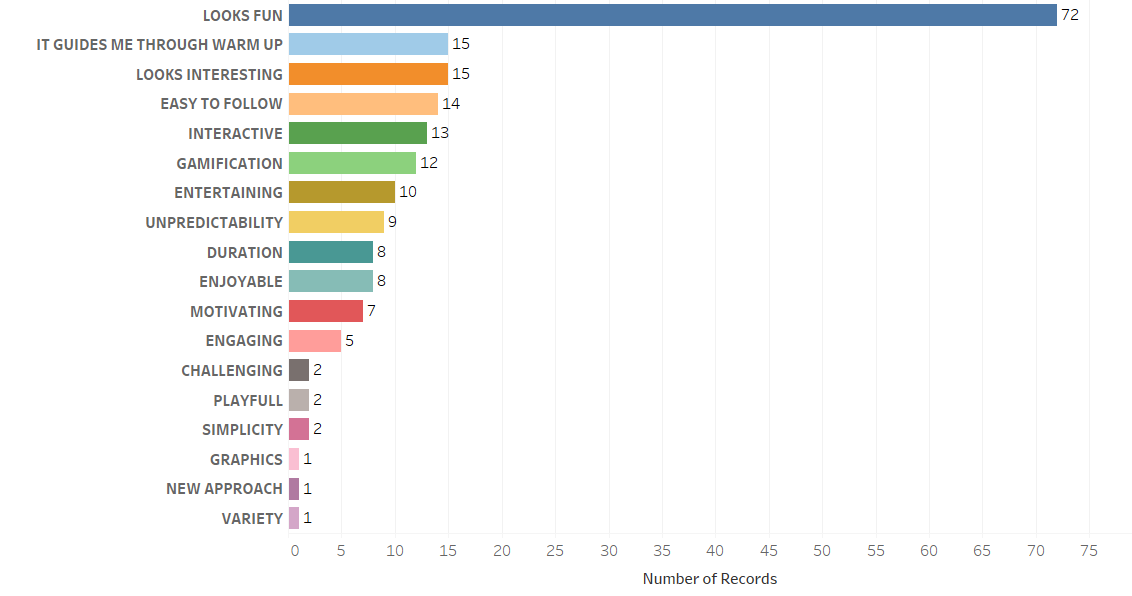
\includegraphics[width=\textwidth]{1_mostImportantFeatures}
    \caption{Aggregated answers for question: ``\textit{What do you think are the most important features of this warm up game that would make you use it?}''}
    \label{fig:1_mostImportantFeatures}
\end{figure}\\ According to the respondents, this warm up game would be the most useful ``\textit{for people that do not warm up or do not know how to warm up}''. This statement aligns with our assumption also. We believe that athletes who rarely or never warm up, as well as athletes who do not know how to perform a warm up routine would benefit from the presented gamified solution for warm up the most. Next, the respondents appreciate the guidance in the game, in a sense that they are instructed to which movements to perform through avoiding obstacles and collecting points:
\begin{itemize}
\item ``\textit{Very simple direction on what to do, once you get the mechanic of what the game is trying to get you to do you don't really have to think much about the varying motions asked of you, you're just trying to hit the orbs by moving your body as necessary.}''
\end{itemize} 
Moreover, they enjoyed the interactive element the game provides through the Kinect sensor, the gamification elements (coins) placed in game scenes and that it is made easy to follow. The obstacles and coins are situated in a way that is easy to understand which movement is required to perform in order to avoid the obstacle or collect more points and, thus, finish the game successfully:
\begin{itemize}
\item ``\textit{The game makes me unconsciously do a proper warm up without me thinking about the procedure and the exercises a lot.}''
\item ``\textit{Performed motions are changing often, definitely more interesting than 30 jumping jacks.}''
\end{itemize} 
Also, some of the respondents appreciate the short duration of the game because it can easily fit in their work out routine. In addition, they point out how this approach could motivate them to start their work out session with warm up and potentially influence the duration of the warm up exercise too. They attribute this to the gamification of the warm up routine and the immersive nature of the game that acts as a distraction, in a sense that, it engages the user and shifts users' focus from a tiresome warm up activity:  
\begin{itemize}
\item ``\textit{It's immersive - it would feel like a game and not a boring warm up routine.}''
\item ``\textit{Engaged without realizing.}''
\item ``\textit{It would increase the duration of my warm up - time passes faster when you are distracted by a video.}''
\end{itemize} 
Furthermore, the short and fixed duration of the game seems to be appealing to the respondents as well. By knowing exactly how long the warm up session will last, they believe that their work our session could be planned better.\\
In order to gain insight into elements of the game the respondents dislike the most, we asked them to point out the features, elements and main aspects of the game they would change or remove completely. These answers gave us more information about respondents' attitudes towards the presented warm up game and their stand about gamified solutions of exercises in general. Based on these answers and suggestions, we added new features and modified exiting ones, in order to have a gamified solution for warm up that fits respondents', and presumably future users', needs the most. Our goal is to offers a solution that can be used before every exercise and sports activity, and having elements and features users expect and desire the most, will make the game more appealing and, thus, more regularly used.
Figure in \ref{fig:2_whatDoYouDislike} shows the summary of responses regarding question ``\textit{What do you dislike about this warm up game with regard to the general idea (using game to motivate users to warm up more regularly)?}''
One of the interesting aspects that was captured during this survey is the main reason why respondents would not use the game. From the results in \ref{fig:2_whatDoYouDislike} we notice that most of the respondents pointed out the hardware (i.e. Kinect sensor, projector and large screens) and its price as the primary argument for not using the game. Surprisingly, from the video that was shown, the respondents assumed that in order to use the game, one must acquire all the necessary hardware and use the game at home before the sports activity:
\begin{itemize}
\item ``\textit{It's too impractical. I can't find a dark room with a projector before I play football or cricket.}''
\item ``\textit{No way would I warm up in one location (living room) before going to exercise.}''
\item ``\textit{Jumping disturbs the neighbors (next door and downstairs) when living in an apartment; prefer warm up outside}''
\end{itemize} 
Taking this into account, the negative bias is acceptable. However, as mentioned before, the game is intended to be used in gyms, fitness and sports centers, and it is not designed to be a solution for home work outs and exercises.
\begin{figure}[h]
    \centering
    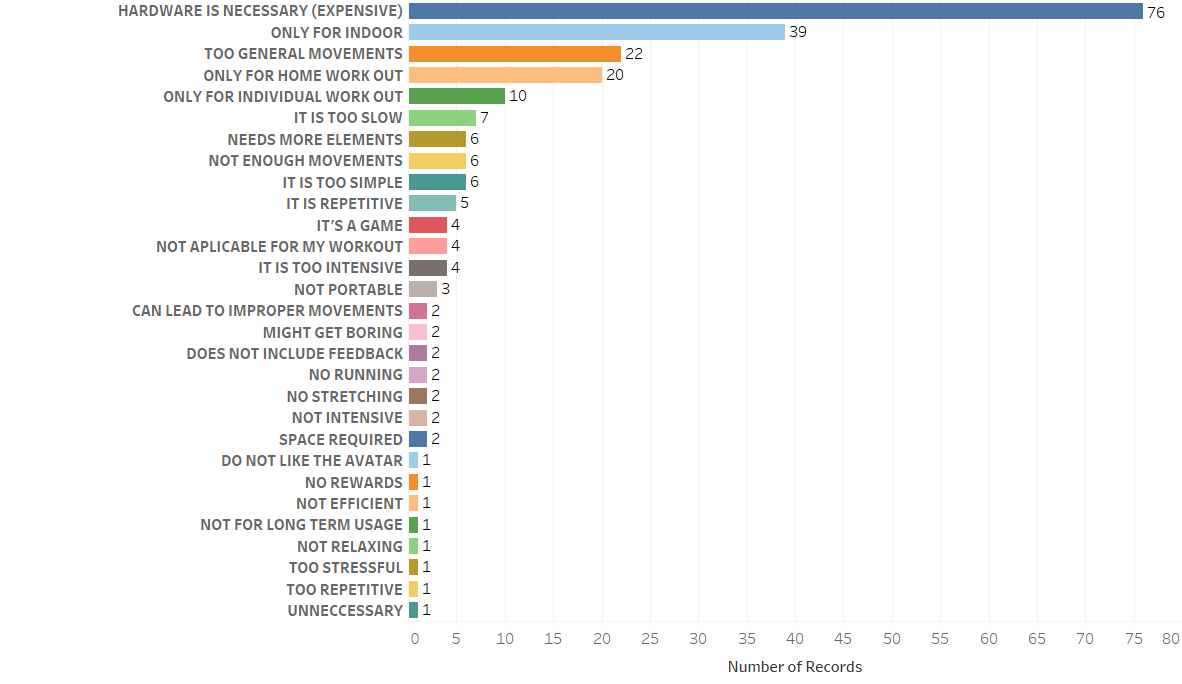
\includegraphics[width=\textwidth]{2_whatDoYouDislike}
    \caption{Aggregated answers for question: ``\textit{What do you dislike about this warm up game with regard to the general idea (using game to motivate users to warm up more regularly)?}''}
    \label{fig:2_whatDoYouDislike}
\end{figure}\\
Since games  work out that are intended to be used at home already exist on the market, our goal is to completely focus on the warm up gamified solution as a preparatory activity before sports sessions and to make it available and usable in places where individuals come to engage in some sort of sports activity. That way, we hypothesize, our approach will be more likely utilized, compared to home work out solutions. In addition to this, respondents who prefer sports and work out exercises outdoor, mostly disliked the fact that the game is intended to be used indoors without any option to be installed and used in open space. This was the second most argued reason for not using the presented game:
\begin{itemize}
\item ``\textit{The issue is that the game has to be setup where I do my sport, which is probably not going to happen (forest)}''
\item ``\textit{You need to do it in a room with a screen and a device, this is a strong constraint if you want to practice sport outdoors}''
\item ``\textit{Most of my warm ups take place outside, and so it may not work outdoors very easily}''
\end{itemize}
They propose having a portable version (mobile application) of the game that can be used without any space or hardware constraints. These recommendation will be further assessed later in this chapter. Furthermore, the respondents pointed out that only few movements (exercises) are required in the game which makes it one-dimensional, neglecting the warm up for arms and upper body:
\begin{itemize}
\item ``\textit{Very limited range of motion, hard to imagine it would capture all required muscle groups one should normally warm up.}''
\end{itemize}
We assume that the reason they find the movements too general and repetitive is because only few exercises and movements were included in the prototype that was presented to them. The prototype had 7 segments and only 4 segments contained obstacles with coins. In the prototype game, the obstacles are avoided and the coins collected using jumps and right and left movements, depending on the position of the game elements. Introducing only limited number of segments and requiring only few movements were determined to be sufficient to present our idea of gamified warm up and assess its general acceptance. For the second release of the warm up game, based on the respondent' answers regarding most common movements and exercises they reported performing during warming up (presented in \ref{fig:5_describeWURoutine}), we extend the number of movements required to carry out in order to successfully finish the game. We believe that we captured and implemented the most common exercises and movements reported by the respondents that are, first, detectable with high accuracy using only one Kinect device and, second, accomplished easily without no prior exercise knowledge or experience. Moreover, we decide to discard and not implement movements that are reported by most of the respondents but require additional equipment in order to be performed, like pull-ups, rowing and rope jumping. 
Next, the respondents mentioned the lack of group (or multiplayer) exercises using the game. Since some of the respondents often engage in group sports, they would expect that the game also includes a version where they can compete with someone while warming up, or just warm up using the game together with the group they exercise with:
\begin{itemize}
\item ``\textit{You could design the game so that it is competitive. You could compete with other players for a high score, and this could become a group activity and become a part of exercise routines. This way, it would also become easier for you to drag someone who doesn't exercise regularly to start doing so.}''
\end{itemize}
This requirement is often mentioned by the respondents. According to the respondents, this feature is necessary for group sports sessions. Introducing this feature could make the game more enjoyable and boost the competitive aspect of the game:
\begin{itemize}
\item ``\textit{It's not practical if you exercise in groups. In this case everyone would need their own screen, which seems like too much of a hassle just to warm up.}''
\end{itemize}
The simplicity of the scenery, used avatar and lack of diversified game elements was also brought up. According to the users, the absence of these elements can potentially make the game monotonous and uninteresting for them after a while. If the game is lacking captivating visuals and scenery, compelling challenges and intriguing story line, users will stop using it after the initial incitement for the game ceases. Taking this into account, we introduce new segments with elements that make the game more appealing and the challenges more attractive. We increase the number of segments from 7 to 20 and completely change the scenery previously presented in the prototype game. Regarding types of exercises performed in the game, many respondents expressed their concerns that stretching exercises are not included in the required movements: 
\begin{itemize}
\item ``\textit{Depending on the efficacy, I would want to incorporate stretching as part of the routine. Even if it was doing some motion detection for active stretching in a direction to pop balloons or something.}''
\item ``\textit{… does not stretch ligaments for my sports (body building)}''
\end{itemize}
Since stretching is part of most respondents' warm up routine, they expect that the game also contains movements and exercises of this type. They propose having movements that focus on whole body stretching, stating it helps them to prepare more for the subsequent physical activity. This statement is surprising since research, as previously discussed,  has never found stretching warm ups to have any benefits in preparing our body for strenuous activity or injury prevention \cite{pereles2012large}. Thus, we choose not to incorporate stretching exercises as required movements in the second release of the game. However, at the end of the game, athletes will be informed about the duration of stretching exercises assumed to be the most beneficial for the subsequent activity. Lastly, the respondents pointed out that the intense focus on the screen could potentially lead to improper execution of the body movement and thus, lead to injuries:
\begin{itemize}
\item ``\textit{When you're not focusing on your movements, you are at a higher risk for injury. Additionally, muscles are more responsive when you're consciously engaging them.}''
\item ``\textit{I worry that I would not use proper technique when playing the game and therefore not successfully warming up.}''
\end{itemize}
They suggest monitoring the correctness of the movements performed by the users and, in case of incorrect ones, inform them in a way it does not affects their performance in the game as a form of a feedback:
\begin{itemize}
\item ``\textit{I think having an interactive screen that takes you through a proper warm up and can educate you on how to properly warm up each muscle and what each movement is warming up would be a great idea.}''
\end{itemize}
Some of the respondents argue that the game requires too general movements and exercises that are too generic and not applicable for the sports they engage in. These athletes usually perform specific warm up exercises that are either too complex to be captured with high precision by the Kinect sensor, or are executed in environment not suited and intended for our gamified solution (e.g. swimming, climbing). In summary, we would like to focus on more general exercises that are simplistic, presumably known by the athletes and can be captured with high accuracy using only one Kinect sensor. Moreover, we want to avoid stretching exercises because they do not provide protection from muscle soreness, they do not seem to contribute to the reduction in the risk of injury and, lastly, there exists insufficient research to support its effectiveness on sporting performance.\\  Figure in \ref{fig:3_featuresToBeUsedRegularly} shows the summary of responses regarding question ``\textit{In your opinion, what features does this game have to possess in order to be used on a regular basis?}''.\\
\begin{figure}[h]
    \centering
    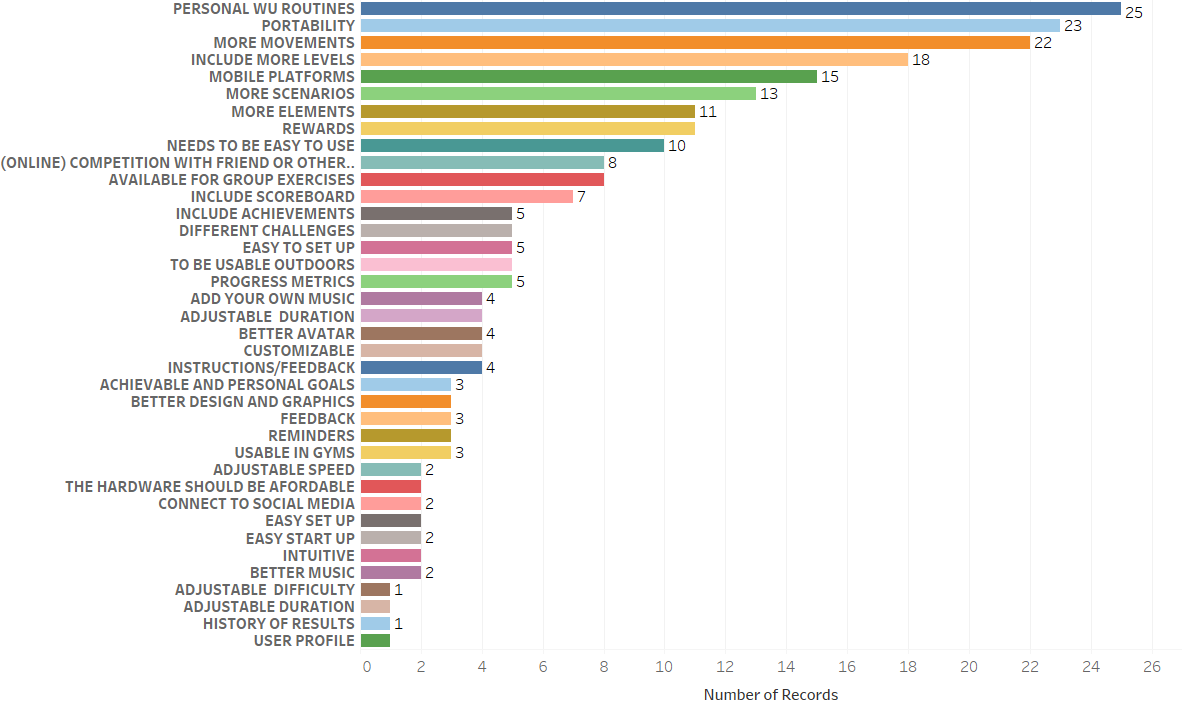
\includegraphics[width=\textwidth]{3_featuresToBeUsedRegularly}
    \caption{Aggregated answers for question: ``\textit{In your opinion, what features does this game have to possess in order to be used on a regular basis?}''}
    \label{fig:3_featuresToBeUsedRegularly}
\end{figure}\\
With this question, our goal was to gain insight into possible features and elements the respondents would look forward to and benefit the most from, in a gamified solution like the presented prototype. Based on these answers, ideas and recommendations we modify our game in order to be more appealing to the future users. From \ref{fig:3_featuresToBeUsedRegularly} we observe that the most of the respondents would enjoy having a gamified solution that is tailored specifically to their needs. That is, the respondents would like to have the option to customize and personalize the warm up routines in the gamified system. According to the respondents, the warm up movements should be adapted to the sport of choice and should also change overtime to avoid the routine being too repetitive.\\
 Namely, the warm up routines should be sports specific, and not general as in the presented video:
\begin{itemize}
\item ``\textit{It would be great if the game had different types of warm ups based on two things:  type of sport activities, which I am about to start (e.g. running, cycling, etc.) and if I have some specific preconditions, like back pain.}''
\item ``\textit{… different levels (for amateurs and for more professionals), different warm ups for different sport activities (e.g. warm up for a run or warm up for a HIIT session)}''
\end{itemize}
Moreover, the game should also take into account any physical injury users have. That is, individuals should be in position to discard some of the movements in case they are not able to perform them. In addition, adjustable game setting are also high in demand. The respondents would rather enjoy having a game with adjustable game elements (segments and avatar), speed, duration and number and types of obstacles. That way, they would be in control of the movements that are needed to be performed, as well as, their intensity and speed. This requirement is actually tightly connected to the one previously mentioned. The respondents would prefer the most to be able to manage and manipulate all the game's features conforming them, by doing so, to their work out preferences. Portable (and mobile phone) version of the game, as in the previous question, is also pointed out by the respondents:
\begin{itemize}
\item ``\textit{As with team sports, location changes weekly so if this game was able to be moved with the team then this would help.}''
\end{itemize} 
Users who engage in sports outdoors or whose work out location changes often, would prefer having a mobile application that helps them warming up. Moreover, the respondents would rather enjoy a game that has more levels with different sceneries and difficulties. Each level, according to respondents, could be at different difficulty level, including new obstacles and, hence, require new movements in order to avoid those obstacles. This way, they believe, the game will stay enjoyable and captivating for a longer period of time:
\begin{itemize}
\item ``\textit{Interesting and achievable goals, something new all the time, new routes, obstacles, etc.}''
\item ``\textit{More movements and as time goes by, the speed of the obstacles you approach should be faster, different and finally a short cool down at the end like just walking for a minute.}''
\end{itemize}
Currently, only one level is available. We believe that introducing multiple levels is an option worth considering. However, we opted for the solution with diversified scenes and elements instead. Gamification elements like scoreboards, awards, achievements and progress metrics were also brought up by the respondents. %should add references to related work here!%
According to the answers, including these elements would make the game more engaging and satisfying. Next, some of them would gladly share their achievements on social media. Hence, connecting the game with social networking platforms would also influence some users to use our gamified solutions. Regarding game graphics and sounds, diversified scenes, being able to choose from multiple avatars and importing custom music playlist was mentioned by the respondents also. Multiplayer version of the game, where one can warm up or compete with someone, according to the respondents, would make the game more appealing and usable.\\ 
Lastly, we asked the respondents to leave comments and recommendations regarding the presented prototype warm up game. We wanted to gain insight into possible features and elements expected by the respondents which could be incorporated in the game. We acquired interesting suggestions and ideas from the respondents, some of which, are implemented in the second version of the game. Figure in \ref{fig:4_recommendations} shows the summary of responses regarding question ``\textit{Do you have any recommendations or suggestions regarding the game?}''\\
\begin{figure}[h]
    \centering
    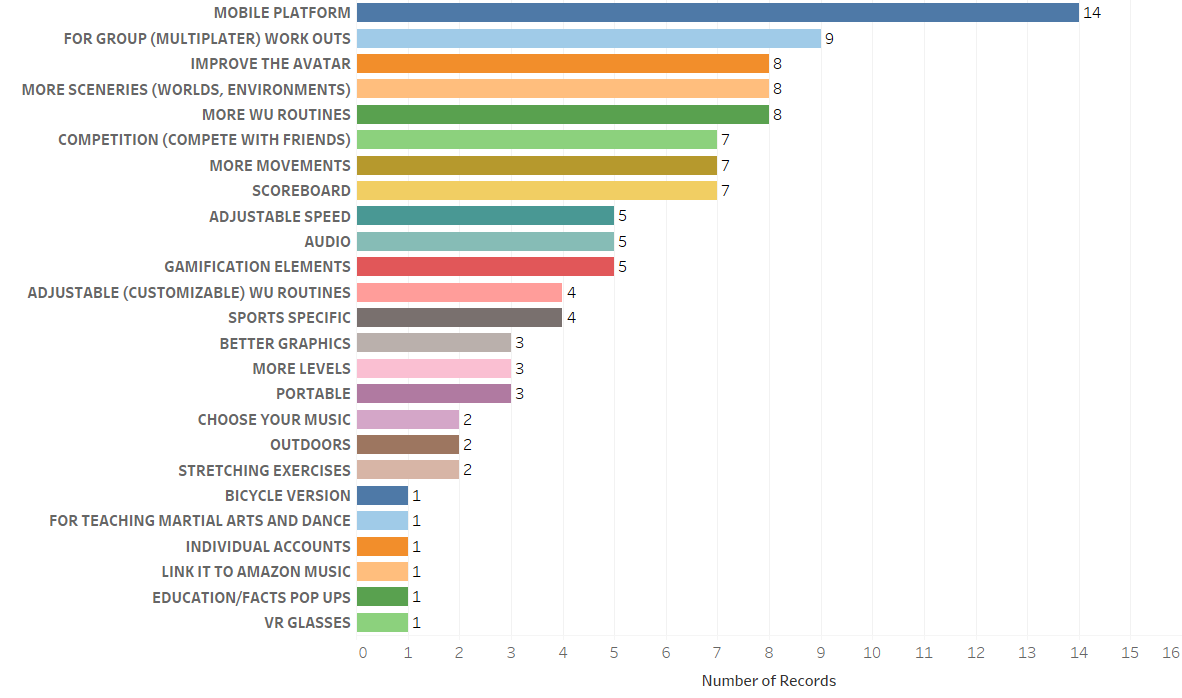
\includegraphics[width=\textwidth]{4_recommendations}
    \caption{Aggregated answers for question: ``\textit{Do you have any recommendations or suggestions regarding the game?}''}
    \label{fig:4_recommendations}
\end{figure}\\ 
From \ref{fig:4_recommendations} we notice that most of the respondents recommended designing and implementing a portable version of the game that is not constrained by any additional hardware currently required for game functioning.\\ \\ \\They suggest having a ``\textit{pocket version}'' the game that can ``\textit{easily be watched on a smartphone}'':
\begin{itemize}
\item ``\textit{Could be on an app form, everyone has a phone they can use; having arrows on the screen about which direction to use. Not as fun but just as effective.}''
\item ``\textit{Well, if the whole same thing can be done on mobile, this will be a great success.}''
\end{itemize}
Furthermore, a multiplayer (group) version of the game where users can compete with others seems to be a very appealing feature most of the respondents brought up: 
\begin{itemize}
\item ``\textit{… I actually think turning it into a competition would be cool where you have different players (and you can add your friends) and then see who completes the warm up with the most points (like Mario Kart or something similar)}''
\end{itemize}
We agree to this suggestion and hypothesize that by creating the option for competitions between athletes, our gamified system would provide users with a solid reason to keep returning to it and, in turn, help with creating a healthy habit of warming up before more strenuous exercises. By keeping track on athletes' performance on how many points have been collected during the warm up session, and also displaying these results in a form of scoreboard, our gamified solution could provide motivation to someone who might not be able to find it on its own.
Most of the respondents did not like the avatar that was used in the prototype version of the game. We expected this reaction since the avatar that has been used did not have humanoid features and was represented using simple lines (skeleton). However, it replicated correctly the user's movement which was our goal with the prototype version of the game: 
\begin{itemize}
\item ``\textit{Having a relatable character that does the workout.}''
\item ``\textit{Obviously it's a prototype, but it'd be better to see a real person or game character in place of a dummy.}''
\end{itemize}
Studies have also found that having avatars that are idealized version of our self can influence how much we enjoy the game and how immersed we become. They continue by saying that people also tend to ``unconsciously conform to the expectations of their avatar's appearances'' \cite{avatar}. Taking this into account, we replace the avatar in second release of the game and chose one that is more relatable and have a correct posture, as suggested by the respondents: 
\begin{itemize}
\item ``\textit{Maybe to think over different positively looking characters with healthy right-looking postures so that a trainee's body can subconsciously copy and remember it.}''
\end{itemize}
Even though many respondents suggested a version of the game with a customizable character or a version of a game with multiple characters one can choose from, the second release of the game contains only one avatar. We want to make the game easy to use and promptly to start. Having implemented the option with multiple and customizable character, we believe, would require more time for initial game start and, thus, increase the duration of the warm up routine altogether. We would not like for the users to spend more time designing more likable avatars than engaging in the warm up routine. This option is, however, very appealing and will be considered for future game releases. Apart from that, many respondents recommended having more movements and exercises one needs to perform in order to complete the game that can be, in the same time, personalized and customizable (sport specific), as discussed earlier.\\In the next section, a short summary of the survey results, together with the changes that will be included in the second release of the Immotion warm up game are presented.
\subsection{Survey Summary and Preliminary Design Implications}
To gain a first insight into acceptance of the Immotion warm up game we created an online survey. The goal of this survey was to explore general work out and warm up habits of the respondents and the general acceptance of our gamified solution for warm up. We hypothesize that gamified warm up solutions can make warm up routines more enjoyable and, thus, motivate individuals to warm up more regularly before physically more demanding exercises. Total number of n = 446 individuals participated in the survey, of which n = 204 (45.7\%) were female and n = 242 (54.3\%) male. The age of the respondents ranged from 17 to 58 with an average age of 30.16 years (SD = 6.49). When asked about their warm up preferences before a physical activity, n = 251 respondents (56.3\%) reported always warming up before physically more demanding exercises (or sports activities), whereas n = 195 (43.7\%) reported not warming up regularly before physically more demanding exercises (or sports activities). This category of respondents have been inquired about the reasons for avoiding warm up exercises before more strenuous physical activity. The results obtained, align with the ones acquired by Fradkin, et al. []. This further justifies the need for educational and motivational solutions, which are enjoyable and easy to carry out, with primary focus on the major muscle groups and benefits of warm up, in order to increase the proportion of athletes who engage in warm up routines before every exercise.\\In the last, third part, of the survey, the respondents were shown a short video with the prototype of the Immotion warm up game. In the prototype game, the players' movements were captured using one Kinect motion sensor and the game displayed on the wall using a projector. In order to complete the game successfully, and consequently warm up, the player was required to avoid obstacles and collect coins. Obstacles were avoided by performing general exercises like squats, jumps and movements to right or left. Total of n = 269 (60.31\%) respondents reported that would use the prototype Immotion game for warming up while n = 177 (39.69\%) would not use the prototype Immotion game for warming up. Out of n = 195 respondents who reported not warming up before sports activities n = 124 (63.58\%) would use the game for warming up. On the other hand, out of n = 251 respondents who reported always warming up before sports activities, n = 145 (57.76\%) would not use the game for warming up. We observe that the general acceptance of the game is positive in both categories of respondents, however respondents who do not warm up regularly would more likely use the proposed solution. Next, all the respondents were asked to give their preferences regarding specific statements we assessed would offer us more insight into respondents' attitudes towards gamification of warm up and our proposed solution. In summary, our warm up game received positive acceptance from all the respondents. However, the obtained results suggest that most respondents who do not warm up regularly would more likely use our gamified solutions as part of their work out (sports) routines compared to the category of respondents who reported warming up regularly, suggesting that it can hypothetically stand as a solution which can increase the proportion of athletes who engage in warm up routines before every exercise or sports activity. Moreover, the results imply that both categories of respondents see the presented gamified approach as a way of making the warm up routine more enjoyable and satisfying and that it could increase the quality as well as the duration of their warm up routines. Overall, the results obtained suggest that the respondents would include our gamified solution for warm up in their exercise routine if they are offered with this option.\\The respondents were further requested to give feedback regarding elements of the game they preferred the most and think a gamified solution like the presented one should possess. In addition they were also asked to point out the features, elements and main aspects of the game they would rather change or remove completely. These answers gave us more information about respondents' attitudes towards the presented warm up game. Based on these answers and suggestions, we added new features and modified exiting ones, in order to have a gamified solution for warm up that fits respondents', and presumably future users', needs the most. Since our goal is to offer a solution that can be used before every exercise and sports activity, having elements and features users expect and desire the most, we believe will make the game more appealing and, thus, more regularly used. The evaluation results from the first survey, as well as respondents' suggestions and recommendations were used to improve the Immotion game in order to be more enjoyable for the future usage.\\ Overall, the results that influenced design decisions for the second release can be generalized as follows:
\begin{enumerate}
\item Game design related
	\begin{enumerate}
		\item Avatar design\\
The respondents argued that the avatar used in the prototype version of the game is not relatable enough. We expected this reaction since the utilized model did not have humanoid features and was represented using simple lines. Taking this into account, we replace the avatar in second release of the game with a humanoid model that is more relatable and have a correct body posture, as suggested by the respondents.
\item Different game sceneries\\ 
According to the respondents, in the absence of the captivating visuals and sceneries, the game can become monotonous and uninteresting after a while. Thus, the scenery is redesigned completely to be visually more appealing and attractive. The game segments with empty walls and boxes that built up the game scenes are removed and the main character is placed in a jungle environment with ancient ruins and various creatures. 
\item Different obstacles\\
In the prototype of the game presented to the respondents, only one type of obstacle was placed in the game segments.  As expected, the respondents argued that the number and types of obstacles need to be increased in order to make the game more interesting and challenging. Hence, we introduce diversified elements that pose as obstacles to be avoided in the second release. We incorporate models of the remains of ancient buildings, old bridges, trees, trunks and different creatures.  
\item Multiple levels\\
The respondents would rather enjoy a game that has more game levels. Each level, according to respondents, could be at different difficulty, including new obstacles and, hence, require new movements in order to avoid those obstacles. We believe that introducing multiple levels is an option worth considering. However, we opted for the solution with diversified game segments and elements instead. The newly introduced obstacles and game elements are generated at random. Hence, each warm up session carried out with our gamified solution is different than the previous, in a sense that the order by which the game segments, and thus the obstacles, are presented to the user are random.  
\item Achievements and rewards\\
The prototype version of the game did not include any rewards or achievements. Including gamification elements like those, according to the respondents, would make the game more challenging and motivate them to take part in it more often. Achievements and awards can be tied to feedback because they are evaluative in nature. By using them, players can reflect on their performance which, consequently increases their perception of competence.  As a result, players' intrinsic motivation can be increased []. In the second release of our warm up game, a new reward system has been introduced. Based on the number of consecutive coin collections, if not hit by an obstacle, the player is awarded by certain amount of additional points. The full description of introduced reward system is detailed in Section XX. 
\item Scoreboard\\
In the second release of our gamified system, we introduce a scoreboard that displays the number of points the player collects. This gamification element is brought up by many respondents as a way of encouraging players to compete. As per various studies, the very presence of a scoreboard can often elicit the desire to play and the goal of advancing in the rankings can serve as a powerful motivator to continue []. 
\item Feedback and metrics\\
The respondents also suggested that the game should monitor the correctness of the movements performed by the users and, in case of incorrect ones, inform them in a way it does not affects their performance in the game. The feedback should, also include different metrics concerning users' energy and calorie expenditure as well as which muscle groups are used in certain movements during the game. Although this suggestion is interesting, we decide not to include direct feedback or metrics during the game. We believe that having all these metrics displayed during the game would be a distraction that will negatively impact the player's performance. Additionally, having only one motion sensor, the complete and correct mapping of the player's body and performed movement can be error prone. The only feedback the user receives during the game is in the form of rewards in case the required conditions are met. Out of the requested metrics, after the game has ended, we display the player's calorie expenditure, number of points reached and the current position on the scoreboard.  
The description and in depth overview of the second release of the warm up game is given in section XX.
	\end{enumerate}
\item Game features related
\begin{enumerate}
	\item Customizable game settings (Avatar, Obstacles, Speed, Duration)\\
The respondents would rather enjoy having a game with adjustable game elements (segments and avatar), speed, intensity and duration. That way, they argue, would be in control of the movements that are needed to be performed, as well as, their intensity and speed. That is, they would prefer the most to be able to manage and manipulate all the game's features conforming them, by doing so, to their work out preferences. Even though many respondents suggested a version of the game with a customizable avatar or a version of a game with multiple avatars one can choose from, the second release of the game contains only one. Moreover, we decided that the game segments will not be editable by the players. That is, players will not be in position to remove some of the game segments together with its obstacles. Our goal is to make the game easy to use and promptly to start. Having implemented the option with multiple or customizable avatars and game segments, we believe, would require more time for initial game start and, thus, increase the duration of the warm up routine altogether. The only adjustable game setting in the second release of the game is the duration. Based on the answers regarding most common warm up duration, we allow players to select their preferred warm up duration. The game speed, as in the original version, will increase gradually based on players' performance.  
\item Multiplayer option\\
Most respondents pointed out that the presented solution is not suitable for group (or multiplayer) exercises. Since some of the respondents often engage in group sports, they would expect that the game also includes a version where they can compete with someone while warming up, or just warm up using the game together with the group (or friend) they exercise with. We agree that introducing this feature could hypothetically engage more categories of athletes to warm up regularly, provide users with a solid reason to keep returning to it and, in turn, help with creating a healthy habit of warming up before more strenuous exercises. However, in the second release of the game, only single player option is available. In the survey, more than half of the respondents (n = 251) stated that they prefer exercising alone (56.3\%), n = 86 (19.3\%) with a friend (or friends) and n = 109 in a group (24.4\%). Thus, as being the majority, we decide to adapt this game feature to those athletes who prefer individual work out (sports) sessions and consider the multiplayer version for one of the subsequent game releases. 
\end{enumerate}
\item Required movements related
\begin{enumerate}
\item Increase required movements\\
The respondents pointed out that only few movements (exercises) are required in the game which makes it one-dimensional, neglecting the warm up for arms und upper body. The prototype solution that was presented to the respondents had 7 segments and only 4 contained obstacles and coins which needed to be collected using jumps or right and left movements, depending on the position of the game elements. Introducing only limited number of segments and requiring only few movements were determined to be sufficient to present our idea of gamified warm up and assess its general acceptance. For the second release of the warm up game with increased number of game segments, based on the respondents' answers regarding most common movements and exercises they reported performing during warming up (Figure 10), we introduce new movements required to carry out in order to collect points and avoid obstacles. We believe that we captured and implemented the most common exercises and movements reported by the respondents that are, first, detectable with high accuracy using only one Kinect device and, second, accomplished easily without no prior exercise knowledge or experience. Moreover, the second release will not require movements that are reported by most of the respondents but require additional equipment in order to be performed, like pull-ups, rowing and rope jumping.
\item Sports specific exercises\\
Some of the respondents argued that the prototype game requires too general movements and not targeting muscle groups that are relevant for the sports they engage in. These athletes usually perform specific warm up exercises that require prior knowledge of the exercise in order to be executed correctly, are too complex to be captured with high precision using only one Kinect sensor, or are performed in settings not suited and intended for our gamified solution (e.g. swimming, climbing).  Taking into account the responses regarding types of movements the responses usually perform in order to warm up (Figure 10), and since only limited number of respondents actually engage in specific warm up routines, in the second release of our gamified system we only focus on exercises that are simplistic, presumably known by the athletes and can be captured with high accuracy using only one Kinect sensor.
\item Include stretching exercises\\
Since stretching is part of most respondents' warm up routine, they also expect that the presented solution contains movements and exercises of this type. They propose having movements that focus on the whole body stretching, stating it helps them to prepare more for the subsequent physical activity. However, as previously pointed out, studies have never found stretching warmups to have any benefits in preparing our body for strenuous activity or injury prevention []. Thus, the second release will not incorporate stretching exercises as required movements. \\In the second stage, based on the feedback and reactions received from the respondents in the first stage, we complete the implementation of the second release of our gamified system and conduct a user study in a local fitness center. Our goal is to assess whether athletes would use our gamified solution to warm up and if it can motivate them to engage in warm up exercises more regularly.
\end{enumerate}
\end{enumerate}
Having analyzed all the results and feedback from the online study, we incorporated the discussed changes into the final version of the exergame. The next section discusses in more details all the changes and improvements that were introduced. 


\chapter{Study Design}
\label{chapter:studydesign}
The main goals of this thesis were to:
\begin{enumerate}
\item develop an exergame which can be used for warm up routine before more strenuous physical activity, and
\item evaluate its effectiveness in terms of guiding the user through the process of warming up.
\end{enumerate} In this chapter we outline the research framework, detail the research methods, and discuss the obtained results.
\section{Description of the Experiment}
This section describes the evaluation of the second version of the Immotion exergame. Our study follows a between–subject design with warm up activity (performed while
interacting with the exergame and performed without interacting with the exergame) as the independent
variable. During the experiment, data has been logged, surveys have been conducted, and interviews undertaken. Similarly to the evaluation of the prototype exergame (Chapter \ref{chapter:survey}), the obtained results are analysed in order to determine to which level our proposed solution was effective in the given context and whether it offered a solution to the problem.
\subsection{Introduction and Goals} \label{chapter:goals}
The first study evaluated the prototype exergame. Based on the results obtained, comments, and suggestions, the prototype exergame has been modified to better suit the needs of its future users.\\The primary goal of the second study was to investigate whether our modified exergame solution can be used as an interactive guide for individuals who do not know how to perform warm up routines. In addition, we examined if the exergame can be used as a solution that motivates individuals to warm up before physically more demanding exercises, and provides an enjoyable exercise, game, as well as play, experience. Taking this into account, the research questions we address in this study are as follows: 
\begin{enumerate}
\item \textbf{RQ1: Evaluation of effectiveness} - How effective our proposed solution is in guiding the user through the warm up routine compared to the guidance offered by classic (traditional) methods?
\item \textbf{RQ2: Evaluation of perceived usefulness and ease of use} - How useful and easy to use our proposed solution is?
\item \textbf{RQ3: Evaluation of the usability} - How usable our proposed solution is? 
\item \textbf{RQ4: Evaluation of the game experience} - How enjoyable and entertaining our proposed solution is? 
\end{enumerate}
%http://edutechwiki.unige.ch/en/Usability_and_user_experience_surveys
%http://www.nigelbevan.com/papers/What_is_the_difference_between_usability_and_user_experience_evaluation_methods.pdf
In order to evaluate the effectiveness, perceived user experience, usefulness, and usability of our exergame solution in the given context, the user base is divided into two groups: \textit{exergame (experiment) group} and \textit{video (control) group}. The first, exergame group, interacted with the exergame directly. Contrarily, the video group was presented with the video of a coach (professional) who guided the participant through the warm up routine. This division allowed us to infer the influence of our gamified solution, as well as, to assess the main differences in completing the required activities between the two user groups. 
\subsubsection{Hypotheses}
Based on the research questions outlined in the previous section, the following hypotheses were established to be tested: 
\begin{itemize}
\item \begin{math}H_{1}\end{math}: The exergame itself is sufficient for guiding the player through a proper warm up procedure.
\item \begin{math}H_{2}\end{math}: After the warm up routine is completed by interacting with the exergame, participant's \gls{rom} is increased.
\item \begin{math}H_{3}\end{math}: Participants had a more positive perceived warm up experience when using the exergame compared to the participants not using the exergame.  
\item \begin{math}H_{4}\end{math}: Participants warm up longer when guided by the exergame.
\end{itemize}
\subsubsection{Apparatus}
The experiment was conducted in the laboratory room in DFKI. The laboratory with the hardware used in the experiment is presented in Figure \ref{fig:lab1}.\\ 
\begin{figure}[h]
    \centering
    \includegraphics[width=0.9\textwidth]{Room1}
    \caption{The laboratory where the experiment has been conducted.}
    \label{fig:lab1}
\end{figure}\\
The following equipment has been used during the experiment:
\begin{itemize}
\item Two Kinect for Xbox One (2.0 2013) motion sensing input devices by Microsoft. One used for movement detection and controlling the exergame avatar and one for recording the experiment.
\item NEN Steam Machine (processor: Intel Core i5-6400T quad-core, 2.2 GHz, up to 2.8 GHz; graphic card: GeForce GTX 960) running the game engine.
\item Projector used to display the game (video) on the wall in front of the participant.
\item Microsoft Band used for gathering skin resistance data.
\item Polar H7 Bluetooth Heart Rate Sensor for heart rate monitoring.
\item Camera for taking photos of participants' facial expressions during the warm up procedure.
\item Medical goniometer used for measuring participants' \acrshort{rom}.
\end{itemize}\pagebreak
Both Kinect motion sensors have been placed in front of the display panel facing the participant playing the exergame or following the video. The participant was instructed to keep at least 2 meters distance from the sensor during the gameplay. This distance was the most optimal in order for the system to function properly in terms of skeleton tracking.
We used a projector in order to display the exergame and video to the participants that was placed above the user so it did not interfere with the game flow.
\subsection{Methods} 
In this section we outline the methodology adopted for the Immotion exergame evaluation. For this purpose we utilized a between-subject design with two groups of subjects. We opted for this approach since it lowers the chances of participants suffering of boredom after series of tests and skewing the results by becoming more accomplished through practice and experience. 
\subsubsection{Participants}
The study has been conducted on \displaydate{date1} and \displaydate{date2} in DFKI \footnote{Deutsche Forschungszentrum für Künstliche Intelligenz GmbH (DFKI) }. All participants were required to report to the laboratory in gym based clothing, preferably shorts and t-shirt, and all of them performed the required tests in the same location using the same equipment. Before the study, each participant signed a consent form. Our subject group included 10 participants, of which 2 were female and 8 were male. Participants were on average age \begin{math}M = 26.7\end{math} years old (\begin{math}SD= 1.77,  x_{max}=30 ,x_{min}= 24 \end{math}), with different levels of education, such as Bachelor's degree (n = 4). All participants were students from Saarland University. The participants reported no physical impairment at the time of participating in the study. For recruiting participants, posters were distributed in print, and sent through social media and email (Appendix \ref{appendix:posters}). Each participant was given 10 euros in cash for taking part in the study.\\\\ All of the participants were amateur athletes. Three participants reported to exercise 1 to 2 times per week, 4 participants 3 to 4 times per week, 1 participant 5 to 6 times per week, and 2 participants 7 to 8 times per week. Only 2 participants reported engaging in sports activity with duration less than 1 hour. The rest of the participants reported engaging in sports activities with duration more than 1 hour. The most common exercises the participants reported to engage in were sit-ups, pull-ups, push-ups, squats, weight lifting, and running outdoors and on the treadmill. The majority of the participants (n = 7) stated to engage in physical activity alone, while only 3 participants reported enjoying sports activities that are performed in a group. Out of 10 participants, 3 reported not engaging in  \acrshort{wu} before sports sessions. \\The most common reasons not engaging in \acrshort{wu} reported by the respondents were time constraint, the monotonous and tiresome nature of the warm up procedure, how the warm up procedure represents an insignificant and negligible activity, and lastly, that no one warms up either. Regarding duration of the warm up session, 6 participants reported spending less than 5 minutes for warming up, while 4 participants reported spending between 5 and 10 minutes on this preparatory activity.\\
\begin{figure}[h]
    \centering
    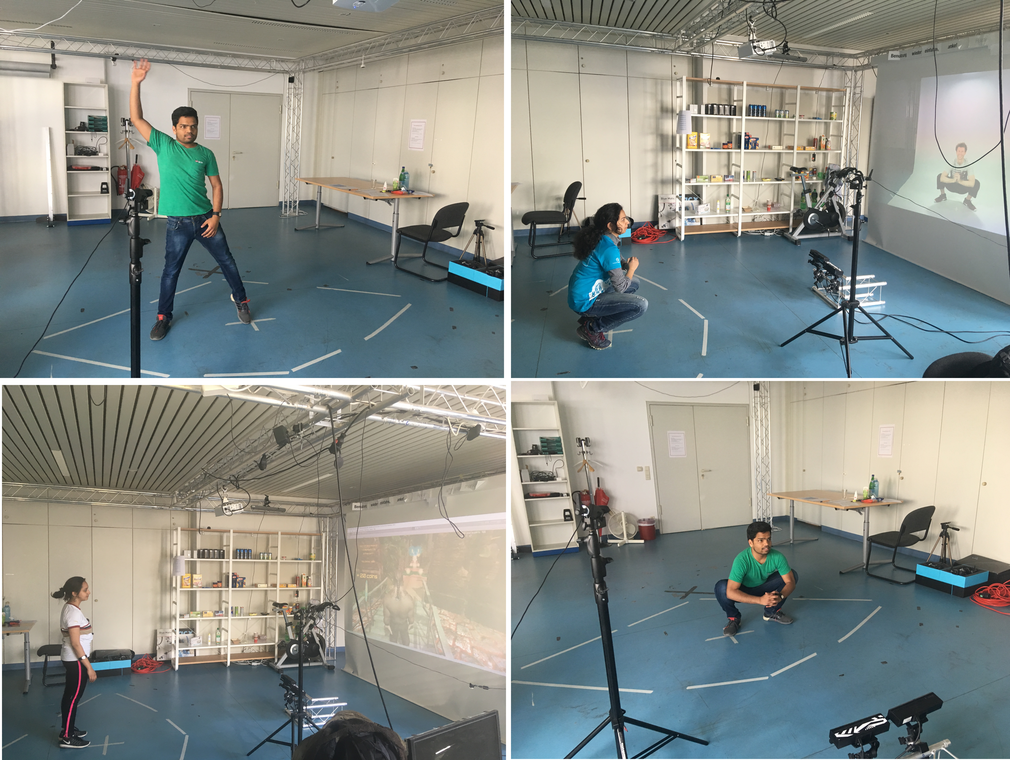
\includegraphics[width=0.9\textwidth]{participantExperiment}
    \caption{Participants during the experiment performing the warm up procedure.}
    \label{fig:participants}
\end{figure}\\
Out of all the participants, 7 stated that they engage in sport specific warm up, whereas 3 reported engaging in general  (non-specific) warm up exercises. Half of the participants (n = 5) stated that they do not enjoy warming up in a group. When inquired about preferences regarding warming up when given instruction, 6 participants stated they prefer warming up when given instructions, while 4 participants stated they do not prefer warming up when given instructions. The engagement in playing video games varies among the participants: 1 plays video games daily, 1 few times per month, 1 once per month, 3 few times per year, and 4 once per year or less. The most common game types among participants were racing (n = 5) and sports games (n = 4). In addition, when inquired about their previous experience with Microsoft Kinect games, only 1 participant reported having a lot of experience with games in this area. The rest of the participants reported having either non or some experience with Kinect related games.
\subsubsection{Conditions}
First 10 participants who applied for the experiment have been accepted. These participants were sent a pre-test questionnaires (\acrshort{bsa}, \acrshort{parq}, and a Demographic questionnaire) that needed to be completed before coming to the experiment. Based on the answers given, the participants were assigned to the video or the exergame group. Each assigned participant took part in a single test session one hour in duration. During this session, all the participants  performed one warm up session, after which they completed a set of questionnaires. \\Two conditions were evaluated:
\begin{enumerate}
\item Warming up with the exergame guiding through the warm up procedure, projected on a wall in front of the participant.
\item Warming up with a video of a professional (coach) guiding through the exact same warm up procedure as induced by the exergame, projected on a wall in front of the participant.
\end{enumerate}
Depending on the group, each participant performed exercise that represent one of the condition.
\subsubsection{Video and Exergame Group}
The participants were assigned to the video or exergame group based on the answers provided in the self-reported questionnaires that were sent to them before the experiment. The surveys assessed participants' perceived physical fitness level, warm up preferences, and previous exergames experience.
\subsubsection{Measures and Metrics}
Two separate sets of questionnaires were administered, one
prior to the experiment session and one post the session in order to gather self-reported user perception data.
The pre-test questionnaires focused on participants' demographic information, overall physical and psychological abilities, hours spent on exercise, frequency and activity
of warm up procedures, extent of video gameplay, and reason for playing. The pre-test questionnaires were as follows:
\begin{itemize}
%https://www.researchgate.net/publication/320572645_Exergaming_Feels_good_despite_working_harder
\item \textit{Health status}. The current health status of the participants has been assessed via the \gls{parq}, which consists of seven dichotomous items \cite{thomas1992revision}. The individual response patterns were used in order to assess if participants were physically able to perform the warm up session. 
\item Demographic survey with questions regarding warm up preferences and previous exergame experience.
\item \textit{Physical activity screening}. Pre-study physical activity levels have been assessed with a standardized questionnaire  \gls{bsa} \cite{fuchs2015messung}. Participants were instructed to indicate for how many minutes per week they performed everyday physical activities (e.g., taking the bike to work; taking a walk) in average during the last four weeks. 
\end{itemize}
The second set of questionnaires have been administered after the completion of the warm up procedure. In these questionnaires participants' level of exertion, emotional state, and game experience have been assessed. The questionnaires were as follows:
\begin{itemize}
\item \textit{Perceived exertion}. For assessing the perceived exertion of the warm up session, the \gls{rpe} has been utilized \cite{borg1998borg}. The perceived exertion reflects how difficult and strenuous the performed warm up exercise feels to the participants, combining all sensations and feelings of physical stress, effort, and fatigue.
\item \textit{Emotional state}. The pleasure, arousal, and dominance associated with a person's affective reaction to a wide variety of stimuli has been assessed with \gls{sam} \cite{bradley1994measuring}. 
\item \textit{Enjoyment of the physical activity}. To test the enjoyment of the physical activity performed, in this case the warm up procedure, the \gls{paces} has been used \cite{kendzierski1991physical}. 
\item \textit{System usability}. For assessing the exergame's instrumental qualities (e.g. controllability, effectiveness, learnability), the \gls{sus} has been used.
\item \textit{Enjoyment of the play}. In order to measure the play enjoyment and experience, the \gls{pes} has been utilized  \cite{pavlas2012play}.
\item \textit{The Gamification User Type}. In order to determine participants’ personality types based on their preferred actions within the game \cite{tondello2016gamification} the participants completed an online survey \cite{userTypeTest}.
\end{itemize}
During the experiment, the following metrics were collected from each participants:
\begin{itemize}
\item \textit{Range of motion}. The participants' \acrshort{rom} has been measured before and after the warm up routine using goniometer.
\item \textit{Heart rate}. The participant's heart rate data has been captured and the measured during the warm up procedure using Microsoft Band.
\item \textit{WU Duration}.  The duration of the warm up exercise has been measured in both the condition.
\item \textit{Skin resistance}. The participant's skin resistance data has been captured and the measured during the warm up procedure using Microsoft Band.
\end{itemize}
The warm up routine performed by the participant has been recorded using a second Kinect sensor for further analysis of performed movements. The questionnaires used in the study can be found in Appendix \ref{appendix:questionnaires}.
\subsubsection{Tasks}
In order to interact with the gamified system, the participants in the exergame group were required to perform a set of general movements. By performing these movements, the participant controlled the game avatar and, by doing so, attempted to avoid obstacles and collected coins. Based on the data and feedback gathered from the first study, we limited the movements the participants needed to perform in the exergame. In accordance with a fitness expert we have selected a set of movements that are simplistic enough to be accomplished easily without prior exercise knowledge or experience. These movements were: 
\begin{itemize}
\item right hand movement up,
\item left hand movement up,
\item jump right,
\item jump left,
\item jump up, 
\item star jump, and
\item squat.
\end{itemize}
Participants who were in the video group were required to perform the same set of general movements. However, they had to follow a video and did not interact with the exergame directly. The video was a recording of a professional (coach) who guided the participants through the warm up routine. We have recorded the warm session with the coach before the study. The movements the coach executed have been induced by interacting with the exergame. Thus, by following the video, the participants in the video condition executed the same movements in the same order as the participants in the exergame group who interacted with the exergame.
\subsubsection{Procedure}
The study protocol was reviewed and approved by an institutional ethics committee (Appendix \ref{appendix:ethicalReviewBoard}). For data collection, we used a  paper and pencil as well as \textit{Google forms} questionnaires. Before the experiment, the lab environment has been set up. The Kinect sensor was placed in a correct position and turned on. The PC running the software was started and the projector is enabled. In each session only one participant was present and guided by the researcher.\\The activities each participant followed were:
\begin{itemize}
\item The participant completes the preliminary survey.
\item The researcher explains the sensors and tools that are required for the experiment, after which the participant puts them on. 
\item After the researcher confirms that the sensors are placed in a correct position, we start recording heart rate data.
\item The researcher measures the participant's \acrshort{rom} before starting the warm up procedure. The following \acrshort{rom}'s are assessed: 
\begin{itemize}
\item Left and right shoulder rotation
\item Left and right shoulder extension
\item Left and right hip flexion
\item Left and right hip extension
\end{itemize}
\item After the measurements are collected, the participant rests while the researcher explains what is required from the participant.
\item The researcher gives a general explanation on the benefits of a proper warm up routine before physically more demanding exercise.
\item The participant moves to the spot marked by the researcher.
\item The researcher starts recording the session. 
\item The warm up procedure begins:
\begin{itemize}
\item If this participant is part of the exergame group, the game begins with the \textit{Start scene}. The researcher inputs the participant's name and presses the \textit{Start} button. After 5 seconds, the game proceeds with scenes in which the participant is required to perform specific movements in order to avoid obstacles and collect coins. The duration of the game is not fixed and it is played up to the point when the participant feels warmed up enough. 
\item  In case the participant is part of the video group, the video that displays a coach who instructs the participants which movements need to be performed. As with with the sessions in the exergame group, the duration of the warm up is not fixed and the video is played up to the point when the participant feels warmed up enough.\\
\end{itemize}
\item After finishing with the warm up routine, the participant takes a rest. The data collection is stopped. During this period the sensors are removed from the participant. \item Researcher assesses the \acrshort{rom}  of the participant. 
\item The participant completes the post-test surveys . %https://www.verywell.com/rating-of-perceived-exertion-scale-3119445
\end{itemize}
\subsection{Limitations - Threats to Validity}
Our participant sample has a small size, an unbalanced gender ratio, and a limited age range, which represent a limitation for the study results. Moreover, the arms of the standard goniometer that has been used for measuring participants' \acrshort{rom} were not longer than 12-inches which made it difficult to accurately pinpoint the exact landmark needed for measurement. Furthermore, our results are based on a single experiment only. Hence, the longitudinal effects of the exergame usage cannot be predicted. 
\section{Results}
In the following subsections we present and discuss the results obtained from various questionnaires the participants completed, as well as, from the metrics that have been tracked and analysed during the warm up procedure.\pagebreak
\subsection{Range of Motion}
\gls{rom} has been assessed  for each condition before the warm up session and immediately the participants completed the procedure. For taking the measures a medical goniometer with 1 degree increments has been utilized. The average \acrshort{rom} values with standard errors for each condition before  and after the \acrshort{wu} session are presented in Figure \ref{fig:romExperiment} and Figure \ref{fig:romControl}. \\
\begin{figure}[h]
    \centering
    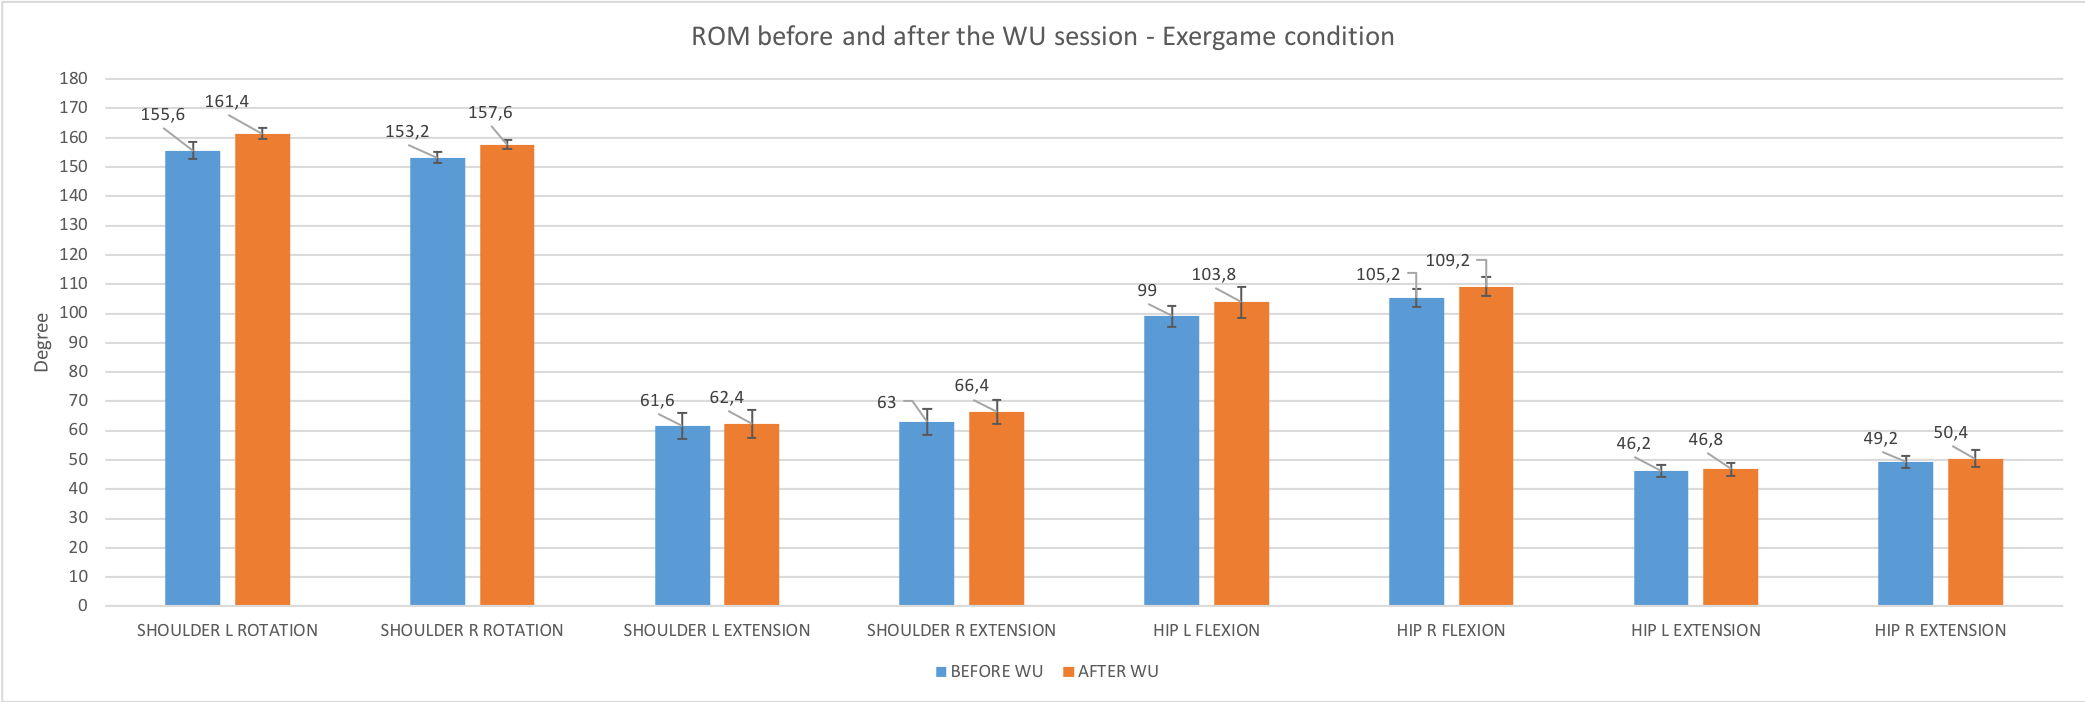
\includegraphics[width=\textwidth]{ROM-Exergame}
    \caption{Summary of ROM results for the Exergame condition.}
    \label{fig:romExperiment}
\end{figure}
\begin{figure}[h]
    \centering
    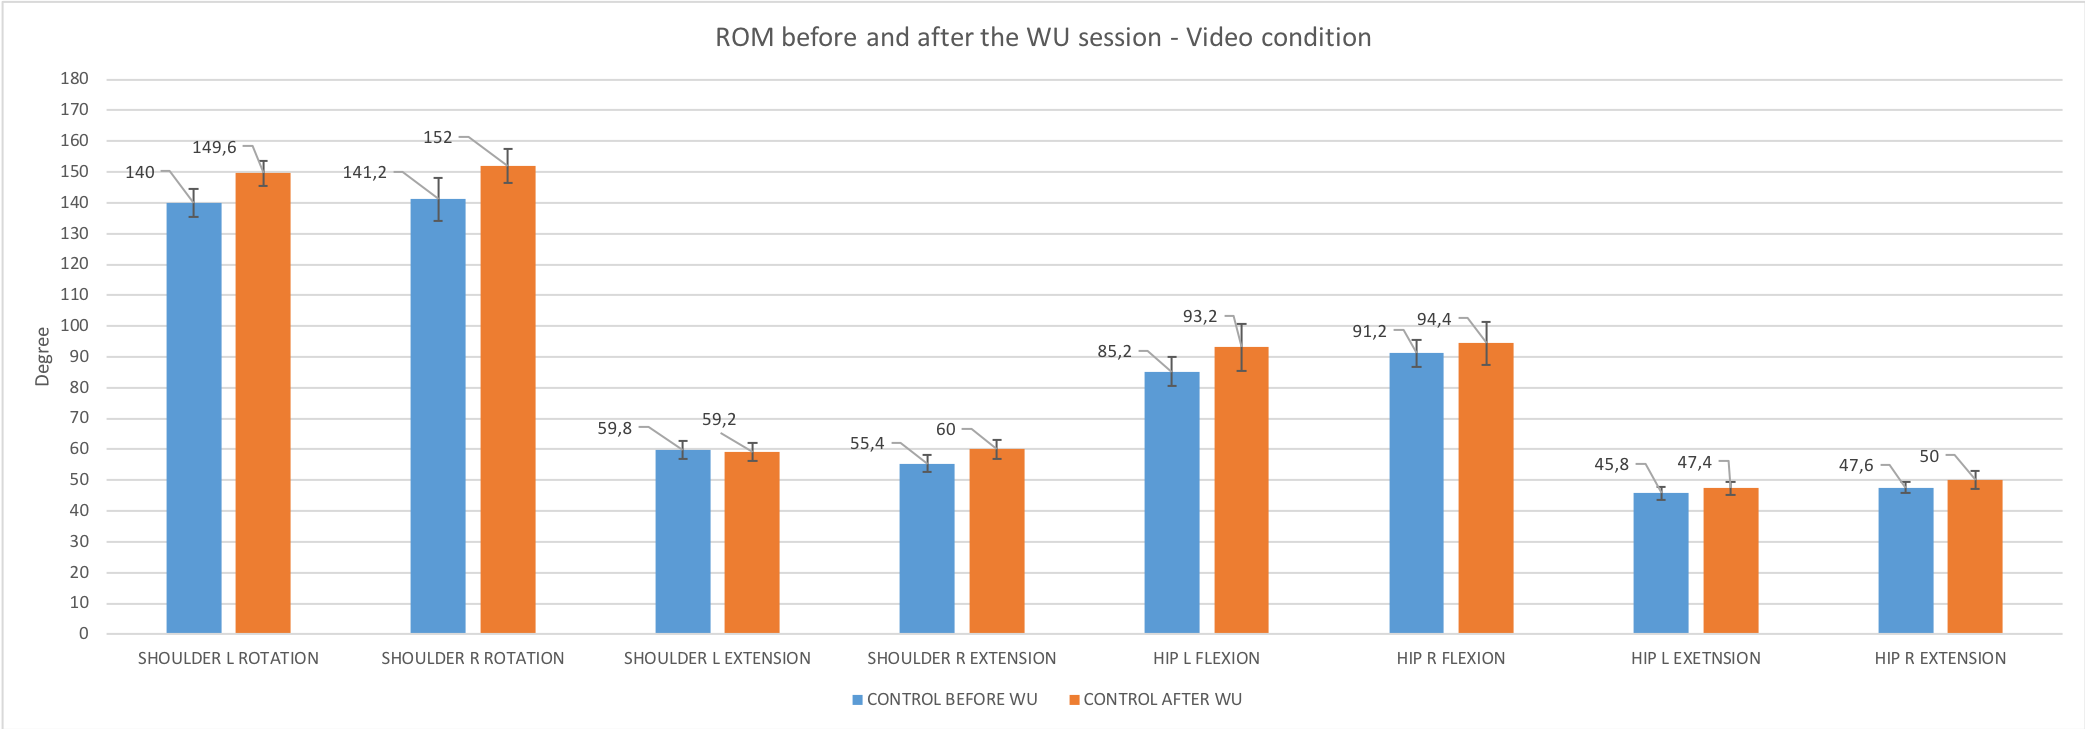
\includegraphics[width=\textwidth]{ROM-Video}
    \caption{Summary of ROM results for the Video condition.}
    \label{fig:romControl}
\end{figure}\\
We observed that the average values after the warm up session for all measured joints were higher in each experiment condition. These increased measures imply that our exergame solution, as traditional warm up procedures, positively affects one's \acrshort{rom}. A paired-samples t-test for independent means was also conducted to compare the obtained \acrshort{rom} results after the warm up session in exergame and video condition was completed. The results showed no significant difference in the scores between exergame and video condition at \begin{math}p = 0.05\end{math} after the \acrshort{wu} session has been completed. These results suggest that even though there are increases in \acrshort{rom} after performing warm up session by interacting with our exergame solution, the increase is similar to the increase in \acrshort{rom} after traditional warm up session. 
\subsection{Warm Up Duration}
The duration of the warm up session has been measured from the game or video start until the moment the participant stopped with the warm up session. The participants have been informed to play the game or follow the video instructions as long as they usually spend on warm up session before some physically strenuous activity. As already pointed out, the exergame was designed with an option for the participant to choose the most desirable warm up duration. However, during the study, this option has been disabled, and the participant could interact with the game and follow the video as long as they felt adequate. The average warm up duration for the exergame condition was \begin{math}M = 847.2 \end{math} seconds (\begin{math} SD = 177.7, x_{max}=1122, x_{min}=657 \end{math}), whereas for the video condition was \begin{math}M = 444.2 \end{math} seconds (\begin{math} SD = 94.2, x_{max}= 576, x_{min}= 345\end{math}). The  results with standard errors for each condition are presented in Figure \ref{fig:wuduration}. Based on the results depicted in Figure \ref{fig:wuduration} we observed that the average duration of the warm up session for the participants in the exergame group was significantly higher compared to the duration of the warm up session for the participants in the video group. That is, interacting with the exergame positively influenced the duration of the warm up session for all the participants in the exergame condition.
\begin{figure}[h]
    \centering
    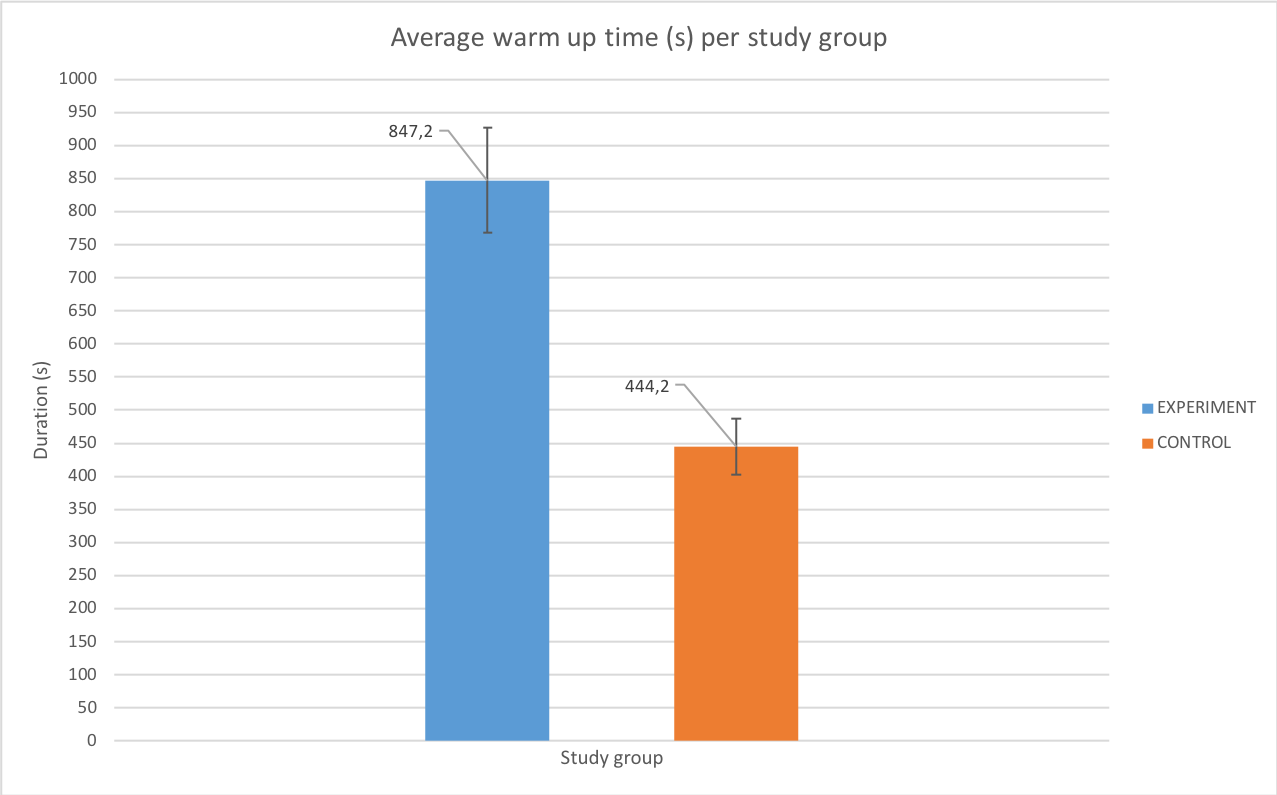
\includegraphics[width=0.8\textwidth]{duration}
    \caption{Average warm up duration with standard errors per condition.}
    \label{fig:wuduration}
\end{figure}\\
An independent-samples t-test was conducted to compare average warm up duration in exergame and video conditions. There was a significant difference in the scores  (\begin{math}\alpha = 0.05\end{math}) for exergame (M = 847.2, SD = 177.7) and video (M=444.2, SD=94.2) conditions; the t-value was 4.48002; the p-value was .001028. These results imply that our exergame does have an effect on warm up duration. That is, the warm up duration increases when performed by interacting with our exergame solution. 
\subsection{Heart Rate}
The heart rate data has been captured and monitored using Polar H7 Bluetooth Heart Rate Sensor and Fitness Tracker in order to determine the exercise intensity. The heart rate has been measured from the beginning of the warm up session until the moment the participant declared being warmed up enough for a subsequent hypothetical physical activity. The average maximum heart rate per participant that is relative to the maximum heart rate computed for each participant based on age, resting heart rate, and heart rate reserve with standard errors is presented in Figure \ref{fig:hrdata} (\begin{math}M_{exp}= 0.919 \end{math},	\begin{math} SD_{exp}= 0.043\end{math}, \begin{math}  M_{con}= 0.84\end{math},	\begin{math} SD_{con}= 0.050\end{math}). The bars presented in Figure \ref{fig:hrdata} are based on  the maximum heart rates calculated for each participant using \textit{Karvonen method}  \cite{tanaka2001age} and obtained by each participant during the warm up session. From Figure \ref{fig:hrdata} is evident that the participants in the exergame condition reached higher relative heart rates based on age groups, compared to the participants in the video condition.\\ %The exergame was more successful in placing more participants in their target heart rate range and in the target heart range for cardio-respiratory benefits.
\begin{figure}[h]
    \centering
    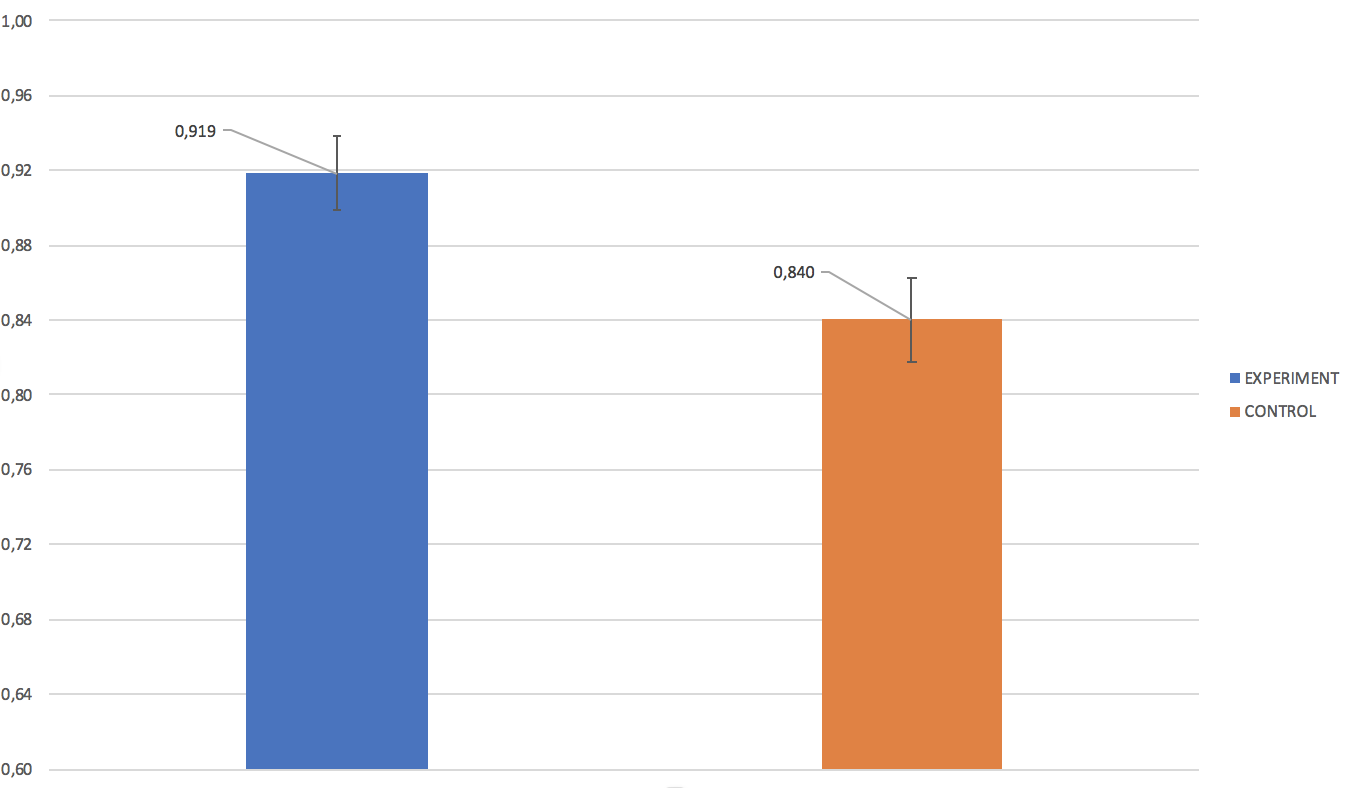
\includegraphics[width=\textwidth]{AverageRelativeHR}
    \caption{Average Maximum Relative heart rate per study group.}
    \label{fig:hrdata}
\end{figure}\\
The individual heart rate data for each participant is depicted in Figure \ref{fig:hrCumulative}  \footnote{The color represents the condition the participant belongs to.}. It can be observed, as previously pointed out, that the participants in the exergame condition who performed a \acrshort{wu} procedure by interacting with the exergame solution, reached higher level of heart rates during the warm up session compared to the participants in the video condition. Furthermore, from Figure \ref{fig:hrCumulative} is evident that the duration of the warm up session for the participants in the exergame group was significantly longer too.
\begin{figure}[h]
    \centering
    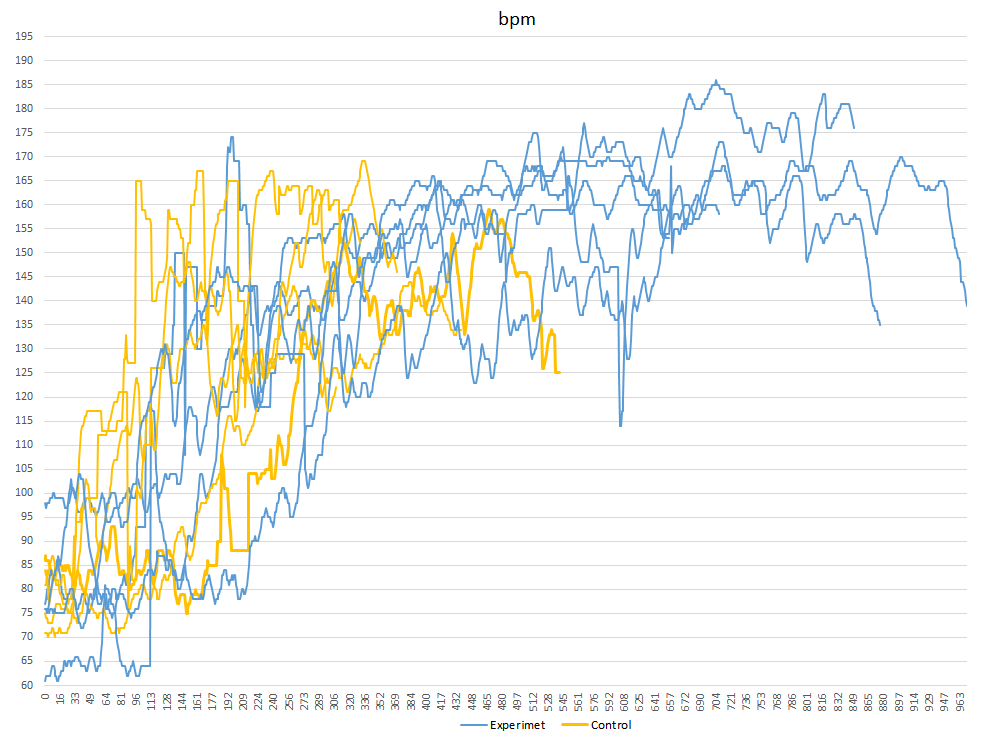
\includegraphics[width=\textwidth]{HRCumulative}
    \caption{Heart rate data for each participant.}
    \label{fig:hrCumulative}
\end{figure}\\
Lastly, we calculated the zones of the target heart rate (\begin{math} T_{HR}\end{math}) for each participant that is based on the maximum heart rate. A number of formulas are used to estimate  \begin{math} THR_{max}\end{math} \cite{heartRate}. Researchers in \cite{tanaka2001age} proposed the following formula for calculating \begin{math}THR_{max}\end{math}:\\
\begin{equation}
THR_{max} = 208-(0.7 * age)
\end{equation}The resting heart rate \begin{math} R_{HR}\end{math} have not been measured during the experiment session. Hence, we utilized the generalized values for \begin{math} R_{HR}\end{math} based on age groups. Since our participant engage in sports activities semi-regularly, we opted for the \textit{average} generalized \begin{math} R_{HR}\end{math} values. \\\\The heart rate reserve (\begin{math} HR_{R}\end{math}) represents the difference between participant's heart rate at rest and heart rate at maximum effort, and has been calculated as follows: \begin{equation}
HR_{R} = THR_{max} - R_{HR} 
\end{equation}The Target minimum heart rate (\begin{math} THR_{min}\end{math}) has been calculated for each participant using the following formula:\begin{equation}
THR_{min} =  HR_{R}*0.5 + R_{HR} 
\end{equation}
Next, the Target moderate heart rate (\begin{math} THR_{mod}\end{math}) has been calculated as follows:\begin{equation}
THR_{mod} =  HR_{R}*0.7 + R_{HR} 
\end{equation}Lastly, the Intense target heart rate (\begin{math} THR_{int}\end{math}), to be reached during extreme-intensity anaerobic exercise, is calculated as follows: 
\begin{equation}
THR_{int} =  HR_{R}*0.85 + R_{HR} 
\end{equation} If the participant's heart rate falls into the middle of the (\begin{math} T_{HR}\end{math}) range, that means the participant is exercising at moderate intensity (roughly 50 to 70\% of \begin{math} THR_{max}\end{math}). In case it verges toward the upper limit, the participant is exercising at high intensity (70 to 85\% of \begin{math} THR_{max}\end{math}). Figure \ref{fig:hrZones} presents the calculated target zones for the participants in both conditions.
\begin{figure}[h]
    \centering
    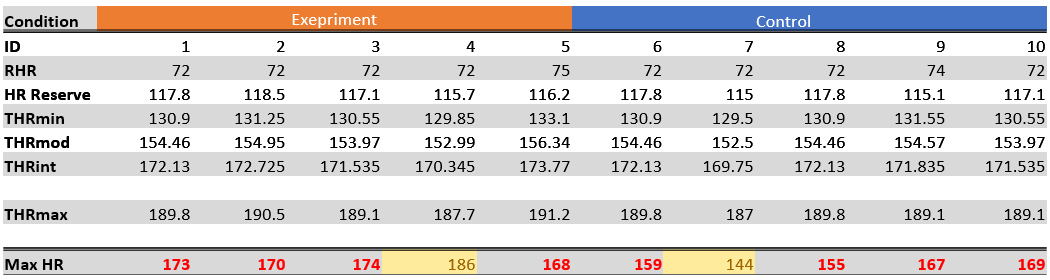
\includegraphics[width=\textwidth]{HRTargetZones}
    \caption{Computed target zones for participants in each condition.}
    \label{fig:hrZones}
\end{figure}\\
It can be observed that the average relative maximum heart rate of the participants in the exergame group obtained during the warm up fall in the middle range of high intensity heart rate zone. Only one participant's (ID = 4) heart rate was close to the maximum target heart rate (\begin{math} THR_{max}\end{math}). On the other hand, the average relative maximum heart rate of the participants in the video group fall in lower and middle range of high intensity, as well as, the upper range of moderate intensity zone. Figure \ref{fig:hrzones} depicts the distribution of average relative maximum heart rates participants reached during warm up session in both condition per exercise intensity zones. Figure \ref{fig:hrzones} depicts three distinct zones (\textit{Low, Moderate, and High (Intense)} heart rate zone) that were computed based on participants' age, resting heart rate, and heart rate reserve. Each zone is represented with different color and the circles, grouped by the condition participants belonged to, show the average relative maximum heart rate during the warm up session. The figure gives a clearer overview of the intensity of the warm up performed in both conditions. It can be observed that the participants in the exergame group reached higher levels of heart rates compared to the participants in the video group. This can mainly be attributed to the warm up duration differences between the conditions. Participants in the exergame condition were engaged in the exergame which shifted their focus from the exertion resulting in longer warm up duration.
\begin{figure}[h]
    \centering
    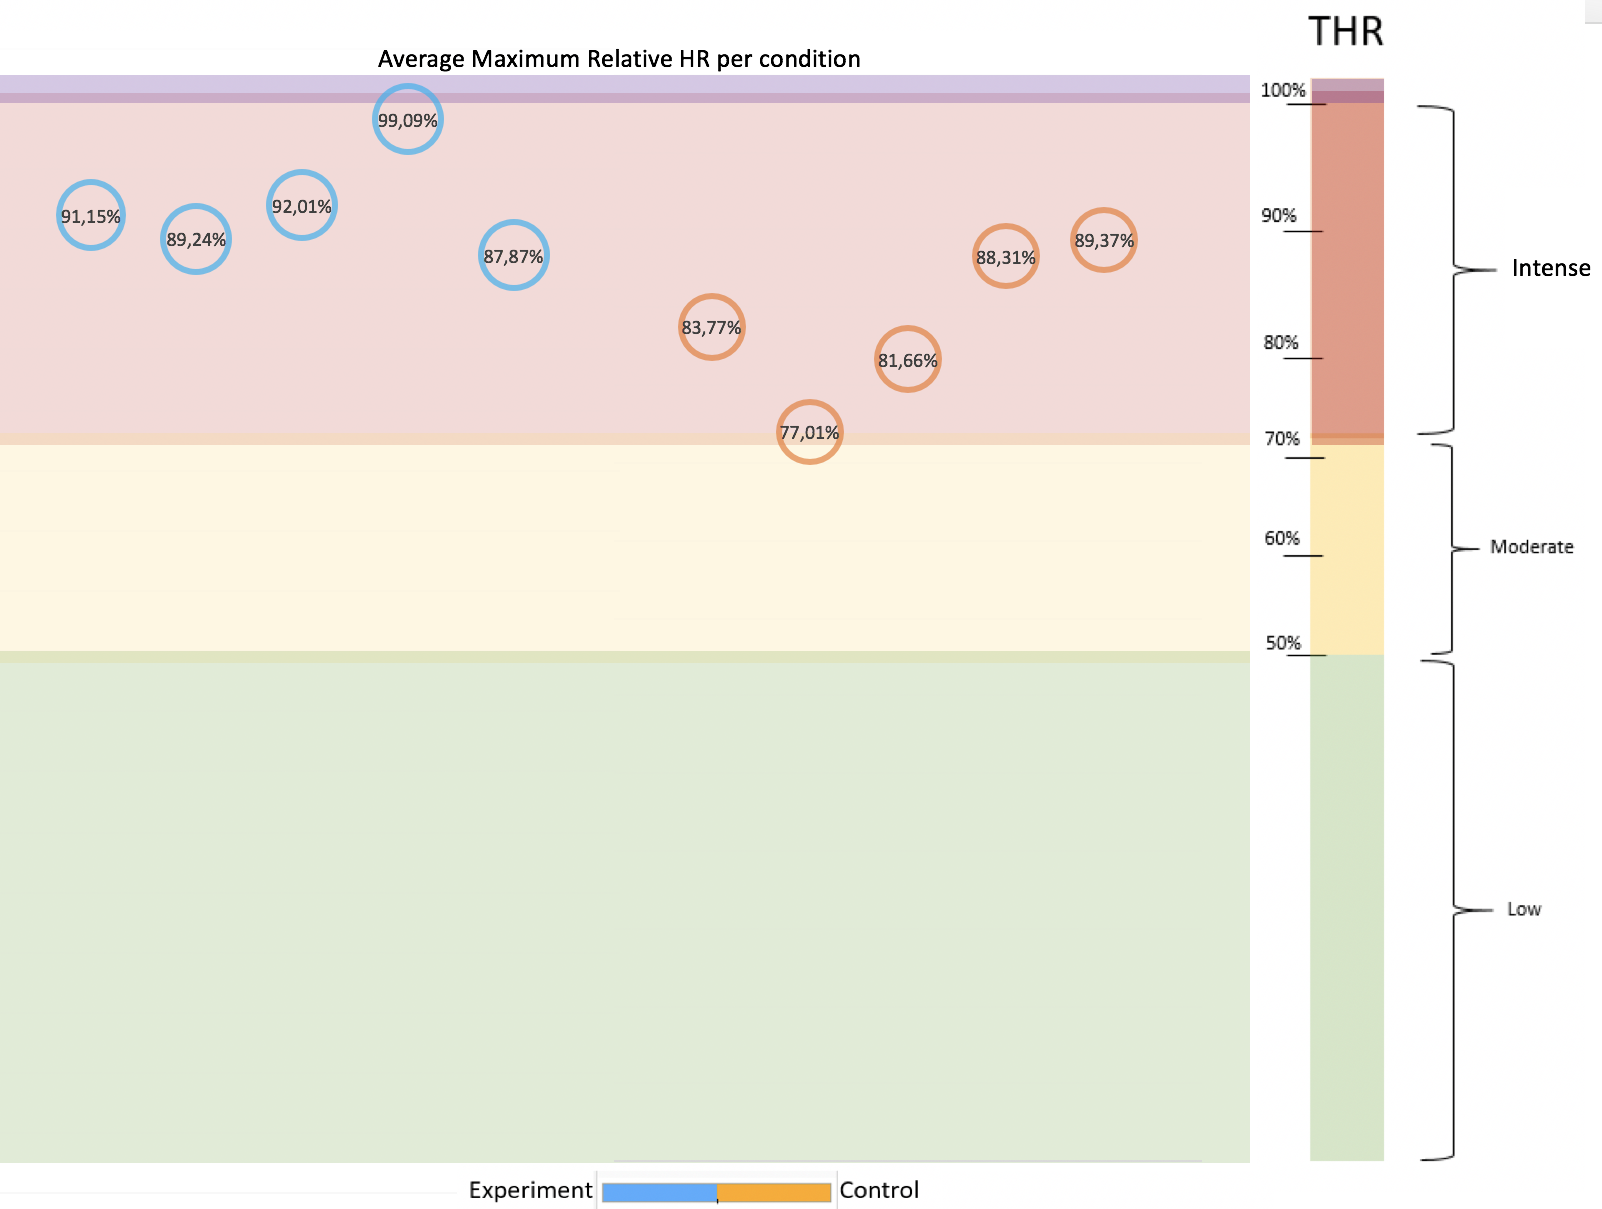
\includegraphics[width=0.9\textwidth]{THR_AVG}
    \caption{Target heart rate with exercise intensity for each participant}
    \label{fig:hrzones}
\end{figure}\\
Overall, we conclude that  participants in both conditions reached an elevated heart rate sufficient to continue with the more strenuous physical activity. The results, however, suggest that the duration  of the warm up session for the participants in the exergame group could be shortened in order to keep the heart rates at moderate levels as recommended by fitness experts. That is, we noticed that some of the participants in the exergame group spent notable amount of time in the intense heart rate zone and were close to reach their maximum heart rate before finishing with the warm up procedure.
\begin{figure}[h]
    \centering
    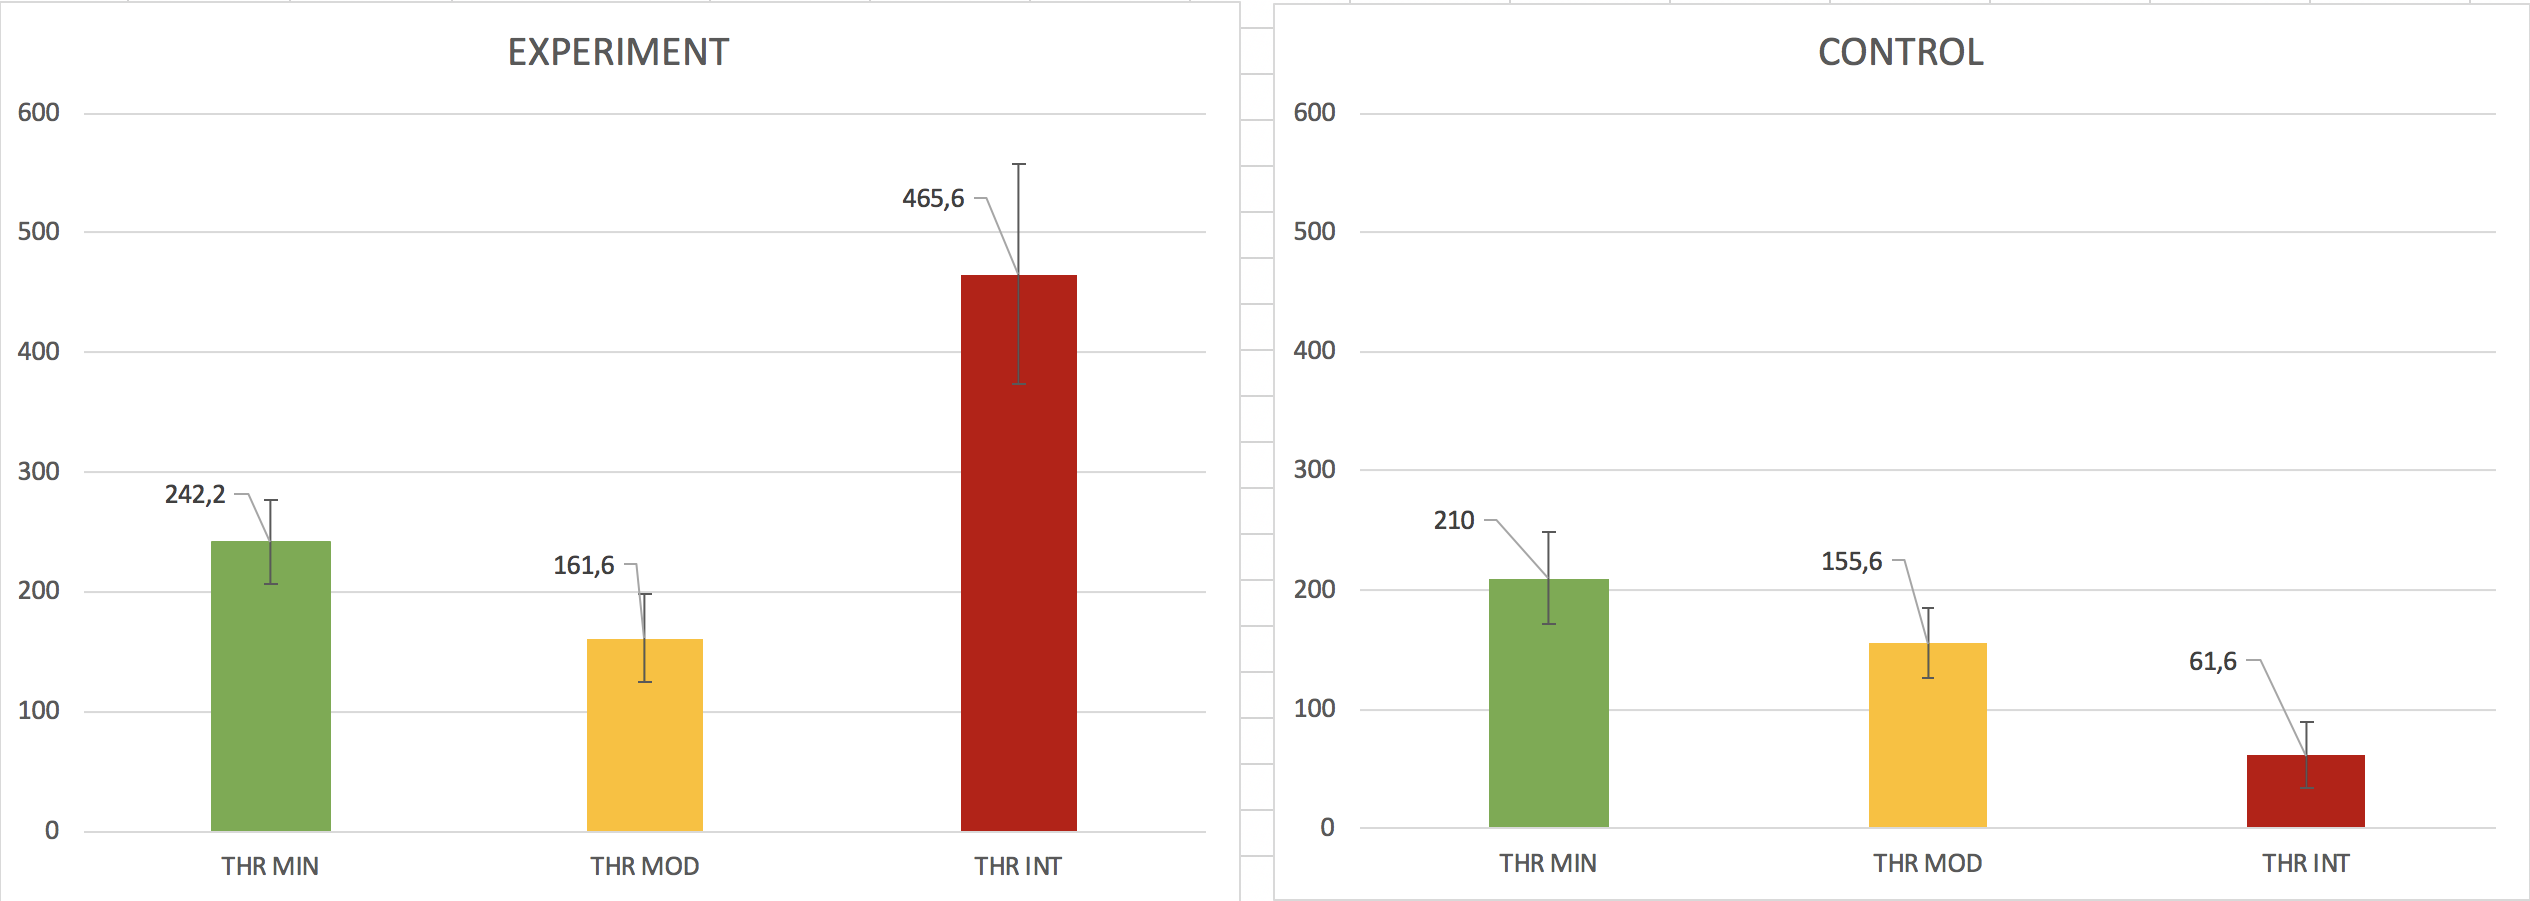
\includegraphics[width=\textwidth]{TimeSpentInZones}
    \caption{Average time spent in zones based on participants heart rate.}
    \label{fig:zonesTime}
\end{figure}\\
It can be observed from Figure  \ref{fig:zonesTime} that the participants in the exergame condition (\begin{math} M_{min}=242.2, SD_{min}=77.7, M_{mod}=161.6 , SD_{mod}=83.001 \end{math} ) spent almost identical amount of time reaching the moderate and intense heart rate as the participants in the video condition (\begin{math}  M_{min}=210 , SD_{min}=86.16, M_{mod}=155.6 , SD_{mod}=64.68 \end{math}). However, the amount of time spent in the high intensity heart rate zone is considerably longer for the participants in the exergame condition (\begin{math}  M_{int}=465.6 , SD_{int}=204.1\end{math}) compared to the time spent by the participant in the video condition (\begin{math}M_{int}=61.6 , SD_{int}=62.48 \end{math}). This can be attributed to two factors. Firstly, the average duration of the warm up session in the exergame condition was longer compared to the average duration of the warm up session in the video condition. Thus, participants spent more time in the intense heart rate zone and were closer reaching their maximum heart rate. Secondly, most of the participants in the video condition stopped with the warm up session before or right after reaching the intense heart rate zone. This impacted and notably reduced the average time spent in the high intensity heart rate zone. Hence, we believe that having an option to choose the warm up duration is a good decision in order to keep athletes' heart rates in the advised heart rate zones. In summary, the results of the heart rate analysis of the participants suggest that exergames can be used to prolong the duration of the warm up session and can motivate athletes to reach higher exertion levels. 
\subsection{BORG Rating of Perceived Exertion}
The \acrfull{rpe} reflects how difficult the performed warm up exercise felt to the participants, combining all sensations and feelings of physical stress, effort, and fatigue. All the participants received standardized instructions and were encouraged to focus upon their overall (whole body) perceptions of exertion. The participants in both conditions reported their perceived level of exertion after completing the warm up procedure.  Figure \ref{fig:borg} depicts the average \gls{rpe}  results for each condition. The average \gls{rpe} score for participants in the exergame condition was   \begin{math}M_{exp} = 13.8 \end{math} while the score for the participants in the video condition was   \begin{math}M_{con} = 12.6 \end{math}. It can be inferred that the participants in the exergame condition reached higher levels of exertion while playing the exergame. For the statistical inference tests of perceived exertion after the warm up sessions the t-tests with the effect size (Cohen`s d) has been used. The results of the analysis showed that a significant difference does not exist  between means of the \gls{rpe} (\begin{math}\alpha = 0.05\end{math})  of the exergame group (M = 13.8 , SD = 1.10, SEM = 0.49) and video group (M = 12.6, SD= 1.67 , SEM = 0.75);  t(8) =1.34164, p = .108274. Whereas Cohen's d was .775. These results suggest that performing \acrshort{wu} procedure while playing our exergame does not have an effect on perceived exertion level. Specifically, our results imply that when participants interacted with the exergame, their perceived level of exertion was higher but not significantly different to the one experienced when performed a standard \acrshort{wu} procedure.\\
\begin{figure}[h]
    \centering
    \includegraphics[width=0.9\textwidth]{BorgSummary}
    \caption{Summary of BORG results for video and exergame group.}
    \label{fig:borg}
\end{figure}
\subsection{Physical Activity Enjoyment Scale}
Given the benefits of physical activity and \acrshort{wu} procedures, we needed to understand better how participants perceived the physical activity they have engaged in. For this purpose we utilized the \acrfull{paces}. The test consists of 18 questions in a 1 to 7 Likert scale that was originally designed to measure positive affect associated with involvement in physical activities in college students \cite{kendzierski1991physical}. The high scores obtained on the positive items and low scores on the negative items indicate a high enjoyment of the physical activity. Whereas, the total enjoyment score is obtained by reversing negative item scores and summing them to positive item scores. We coded participants' responses, where higher scores indicated greater enjoyment, with scores ranging from 18 to 126. The participants in both conditions completed the \gls{paces} after finishing with the \acrshort{wu} session. Figure \ref{fig:pacees} presents the average results for each question per condition. It shows that the participants in the exergame condition rated consistently higher all the questions with respect to the scores of the participants in the video condition. Two questions received notably much higher score by the participants in the exergame condition: \begin{itemize}
\item Q4: ``\textit{I find it pleasurable.}''
\item Q5 ``\textit{I am very absorbed in this activity.}''
\end{itemize} \pagebreak
This suggests that the participants found the exergame very enjoyable to interact with  and, most importantly, the exergame succeeded in immersing the participants sufficiently to shift their focus from the exertion of the exercise making it pleasing and entertaining.
\begin{figure}[h]
    \centering
    \includegraphics[width=0.9\textwidth]{PacesSummary}
    \caption{Summary of PACES results for the video and exergame group.}
    \label{fig:pacees}
\end{figure}\\
Figure \ref{fig:pacesPerCondition} depicts the average scores for all questions per condition. It can be observed that the average score for the video condition is \begin{math}M = 89.8 \end{math} (\begin{math} SD = 11.97, x_{max}= 104, x_{min}= 71\end{math}), which is already high, but for the exergame condition is even higher  \begin{math}M = 114.4 \end{math} (\begin{math} SD = 5.98, x_{max}= 125, x_{min}= 111\end{math}).\\
\begin{figure}[h]
    \centering
    \includegraphics[width=0.9\textwidth]{pacesPerCondition}
    \caption{Average PACES scores for video and exergame condition.}
\label{fig:pacesPerCondition}
\end{figure}\\
Lastly, we compared the means of the exergame (\begin{math}M = 114.40 , SD = 5.98\end{math}) and video (\begin{math}M = 89.80, SD = 11,97\end{math}) group with a paired t-test (\begin{math}\alpha = 0.05\end{math}) and found a significant difference; t(8) = 4.1114, p = .0034. Whereas Cohen's d was 2.5948. Therefore, based on the fact that there was a statistically significant difference between the two conditions, we concluded that warming up by using our exergame solution positively affects the physical activity enjoyment.
\subsection{Self-Assessment Manikin}
All the participants reported their momentary feelings of pleasure, arousal, and dominance using a validated 9-point pictorial rating scale immediately after completing the \acrshort{wu} session using the \acrfull{sam} \cite{bradley1994measuring}. The \acrshort{sam} scale is frequently used to measure emotion in research on gaming \cite{poels2012pleasure} and it is depicted in Figure \ref{fig:samoverview}. The scores in this scale go from 1 to 9 and are classified as being negative (from 1 to 4), neutral (5), or positive (from 6 to 9). The characters presented in the first row in Figure \ref{fig:samoverview} range from sadness and frown to a smile, representing the \textit{valence} dimension. The second row depicts a figure showing a calm, neutral, and passionless face to an anxious and excited face. It represents the \textit{arousal} dimension. The third row represents the \textit{dominance} dimension and the figures range from a very small, insignificant figure to a ubiquitous and pervasive figure. \acrshort{sam} average results calculated for each condition are presented in Figure \ref{fig:sam}. The obtained results indicate slightly elevated scores across the valence and dominance dimensions in the exergame group. On the other hand, the average arousal score in the video group was higher compared to the average score of the exergame group. \\
\begin{figure}[h]
    \centering
    \includegraphics[width=0.85\textwidth]{sam}
    \caption{The Self-Assessment Manikin (SAM).}
    \label{fig:samoverview}
\end{figure}\\\\
For the statistical inference test of the subjective ratings of present emotions after the \acrshort{wu} sessions we performed a t-test and also reported the effect size (Cohen`s d). After the performed analysis, we concluded that a significant difference exists only between means of the \textit{valence} dimension at  \begin{math}p \textless  0.05 \end{math} of the exergame condition (\begin{math}M = 7.20, SD = 0.447, SEM = 0.2\end{math}) and the video condition (\begin{math}M = 6.00, SD= 1.00, SEM = 0.45); t(8) = 2.4495, p = .040, d =1.73\end{math}.  The performed analysis did not show any significant difference between scores in the \textit{arousal} and \textit{dominance} dimensions.\\
\begin{figure}[h]
    \centering
    \includegraphics[width=\textwidth]{SamSummary}
    \caption{Summary of SAM results for video and exergame group.}
    \label{fig:sam}
\end{figure}\\
These results suggest that our exergame does have an effect on participants' feeling of pleasure. Specifically, our results suggest that when our exergame solution is used for warming up before physically more demanding exercise, the pleasure and enjoyment of the activity is higher compared to the one experienced during regular warm up routines.
\subsection{System Usability Scale}
The \acrfull{sus} is a reliable tool for measuring the usability of a system under test. It consists of a 10 item questionnaire with five response options for respondents from \textit{Strongly agree} to \textit{Strongly disagree}. The sum of the 10 items in the questionnaire leads to a general measure of perceived usability of the system. The participants' scores for each question are converted, added together, and then multiplied by 2.5 to convert the original scores of 0-40 to 0-100. Even though the calculated scores are between  0 and 100, these are not percentages and should be considered only in terms of their percentile ranking.\\\\ A \acrshort{sus} score above 68 would be considered above average and anything under 68 as below average. Only the participants in the exergame condition took the \acrshort{sus} questionnaire since only these participants interacted with the exergame system. The summary of the \acrshort{sus} scores for each participant is presented in Figure \ref{fig:sus}. It can be observed that the participants who interacted with the exergame gave the exergame relatively high scores. The  average \acrshort{sus} score for our exergame  was \begin{math}M = 76.7 \end{math} (\begin{math} SD = 8.16, x_{max}= 90, x_{min}= 72.5\end{math}). This implies that our system usability received \textit{excelent} adjective rating and a \textit{B} on a grade scale \cite{brooke2013sus}.
\begin{figure}[h]
    \centering
    \includegraphics[width=\textwidth]{SUSSummary}
    \caption{Summary of SUS results per participant.}
    \label{fig:sus}
\end{figure}\\
The \acrshort{sus} average scores per question are depicted in Figure \ref{fig:susPerQuestion}. It can be observed that the participants found that the various functions in the exergame have been well integrated and that they felt very confident using the exergame. Furthermore, all the participants agreed that people would learn to use the exergame very quickly. Also, they did not find the exergame unnecessarily complex or having any unconsistencies during gameplay. They also thought that it was not difficult or awkward to use, and that getting familiar with the game was pretty straightforward and fast. When asked if they would like to continue playing the game frequently, 3 participants agreed with this statement, 1  neither agreed nor disagreed, and 1 disagreed. \pagebreak
\begin{figure}[h]
    \centering
    \includegraphics[width=\textwidth]{susScoresPerQuestion}
    \caption{Summary of average SUS results for each question.}
    \label{fig:susPerQuestion}
\end{figure}\\ 
\subsection{Play Experience Scale}
The \acrfull{pes} is a valid and reliable 16 items questionnaire with five response options for respondents from \textit{Strongly agree} to \textit{Strongly disagree} \cite{pavlas2012play}. It has been utilized in order to assess play experience, the usability, and the level of enjoyment induced by our exergame. The \gls{pes} scale collects responses across four experiential dimensions: \begin{itemize}
\item \textit{Freedom} captures a state in which an individual is free in a play context to act without any constraints. 
\item \textit{No Extrinsic} addresses a state in which the individual does not feel there are real -world consequences to her play.
\item \textit{Play Direct} addresses the play itself.
\item \textit{Autotelic/Focus}. When experience is autotelic, an individual engages in it solely for its own rewards. That is, the experience is intrinsically motivating.  Focus, on the other hand, targets the states of immersion and concentration during play. It is related to engagement and flow, and the items in this category reflect on the loss of concern and focused concentration.
\end{itemize}
Figure \ref{fig:pesPerQuestion} summarizes the PES results per question for each dimension discussed \footnote{Yellow bars have been reverse-coded.}.
\begin{figure}[h]
    \centering
    \includegraphics[width=\textwidth]{PESSummaryPerQuestion}
    \caption{Summary of average PES scores per question.}
    \label{fig:pesPerQuestion}
\end{figure}\\
In general, the participants enjoyed the play experience induced by our exergame, which can be concluded from high average scores for the questions in each dimension. The lowest scores were obtained in questions that belong to \textit{Freedom} and \textit{Autotelic/Focus} dimensions. The highest scores were obtained in questions that belong to \textit{No Extrinsic} and \textit{Play Direct} dimensions. The scores from \textit{No Extrinsic} dimension suggest that the play induced by our exergame solution was not contingent by external rewards or consequences. That is, the participants felt that there were no consequences to their play, either via evaluative judgement by the researcher or through real-world implications for the \acrshort{wu} performance. High average scores in the \textit{Play Direct} dimension imply that the participants believed they engaged in play as defined by \cite{pavlas2012play} and not work. This information is valuable since it suggests that the warm up induced by our exergame has not been received as a tiresome activity as reported for the standard warm up procedures. On the other hand, relatively lower average scores in the \textit{Freedom} dimension imply that the players felt they have not had total control over the play. When an individual is free in a play context, he or she is not constraind by any means to perform the actions he or she wishes to perform \cite{pavlas2012play}. The following statement received the lowest score in this dimension: 
\begin{itemize}
\item ``\textit{The game gave me freedom to act as I wanted to.}''
\end{itemize} This suggests that certain game elements and constraints prohibited the players to act as they would expected to in similar situation, which in turn negatively impacted the play enjoyment.  In the \textit{Autotelic/Focus} dimension, one question received surprisingly high score.  
\begin{itemize}
\item ``\textit{When I was in the game, I was focused on the task at hand.}''
\end{itemize} This question reflected the state of intense concentration that is related to engagement and state of flow. High average score implies that our exergame succeeded in immersing the player in the activity at such  level, the player's concentration was allocated completely for the play task at hand.  In contrast, the remaining 3 questions in the same dimension received low average scores. However, this dimension measured the autotelic experience induced by the exergame.  Even though the average scores are not extremely low, we cannot claim that the experience was autotelic for the participants and that they engaged in it solely for its own regard. That is, the experience was not fully intrinsically motivating for the participants. The average \gls{pes} scores for each participant are presented in Figure \ref{fig:pes}.
\begin{figure}[h]
    \centering
    \includegraphics[width=0.85\textwidth]{PESSummary}
    \caption{Summary of average \acrshort{pes} score per participant.}
    \label{fig:pes}
\end{figure}\\
As for the previous figure, we can notice the high overall \acrshort{pes} score per participant. This imply that, in general, the participants did enjoy the experience induced by interacting with our exergame solution. Most importantly, by creating an enjoyable experience,  the exergame successfully shifted participants' focus from the discomfort and exertion of the exercise towards the enjoyment of the experience. 
\subsection{Gamification User Types Hexad}
In order to determine participants' personality types according to their preferred actions within the game, each participant that interacted with the exergame completed an online survey that assessed the degree to which they can be motivated by either intrinsic or extrinsic motivational factors \cite{tondello2016gamification}. We chose to utilize this framework and the survey since it is more effective than directly asking users about design elements. Our primary goal was to understand more about user psychology in a gamified context rather than just determining game elements the user enjoys the most. \\The survey was completed after the \acrshort{wu} session and consisted of 24 items which assessed the person's \textit{Hexad user type}, derived from the three types of intrinsic motivation from \acrshort{sdt}, namely relatedness, competence, and autonomy. Figure \ref{fig:playerTypes} depicts the obtained results. 
\begin{figure}[h]
    \centering
    \includegraphics[width=.90\textwidth]{PlayerTypes}
    \caption{The Hexad user types of the participants in the exergame condition.}
    \label{fig:playerTypes}
\end{figure}\\ It is necessary to point out that even though users are likely to display a principal tendency or user type, in most cases they will also be motivated by all the other types to some degree. Based on the results obtained, we found that 2  of our participants can be categorized as \textit{Achiever} player type. This player type is mostly motivated by various challenges that allow them to test their knowledge and apply it in order to solve a problem. Overcoming different challenges will make them feel they have earned their achievement. They are, furthermore, highly motivated by game quests which give them fixed goal to achieve. Leaderboard and different progress and feedback mechanisms can further motivate this player type to perform better in the game. \textit{Free spirit} user type tendencies have been displayed by 2 participants. This user type is mostly motivated by exploration and multiple branching choices. They enjoy being able to choose their path and destiny, whereas the choice has to be or at least feel meaningful to be the most effective and appreciated. One of them has also been categorized as a \textit{Player type}, which is often highly motivated by game rewards, points, leaderboards, and badges. Lastly, 1 participant displayed \textit{Philantropist} player type tendencies. This player type is mostly motivated by meaning and purpose. That is, they have to feel they are part of something greater than themselves, where they can help other players or contribute to the gaming community. \\ 
The analysis of player types suggests that, as pointed out by \cite{hamari2014does} in their review of peer-reviewed empirical studies on gamification, the effects of the utilized gamification elements are greatly dependent on the context in which they have being implemented and on the users using it. That is, our exergame solution should target specific player types that can be motivated and immersed by the elements used in the exergame. These player types should be \textit{achievers}, \textit{players}, and \textit{free spirits}.
\subsection{Post study questionnaire}
As a last step in our experiment, the participants in both conditions completed  a \textit{Post study} questionnaire with five response options from \textit{Strongly agree} to \textit{Strongly disagree} that evaluated the participants' overall satisfaction with the exergame and video, and further discussed specifics the participants enjoyed and disliked the most. Participants completed a questionnaire with questions created specifically for one of the condition. Moreover, the questionnaire for the exergame condition contained 3 additional open ended questions regarding possible improvements of the tested exergame. In the following subsections, the results for each condition will be presented and further discussed.
\subsubsection{Post study questionnaire for the exergame condition} 
The following statements have been evaluated with the participants in the exergame condition:
\begin{itemize}
 \item \textit{Using the exergame is a fun way to warm up.}
 \item \textit{Using the exergame is an exciting way to warm up.}
 \item \textit{The exergame is challenging to play.}
 \item \textit{The exergame is frustrating to play.}
 \item \textit{The exergame is easy to learn to play.}
 \item \textit{The exergame is boring to play.}
 \item \textit{I liked the avatar design.}
 \item \textit{The in-game (live) scoreboard motivated me to play longer.}
 \item \textit{The possibility to collect more coins motivated me to move more.}
 \item \textit{I did not care if hit by an obstacle.}
 \item \textit{The exercise movements induced by coins and obstacles felt intuitive and came naturally.} 
 \item \textit{I would consider using the exergames in order to warm up before physically more demanding exercise.}
\end{itemize}
The scores for each statement are presented in Figure \ref{fig:poststudyexperiment}.\\
\begin{figure}[h]
    \centering
    \includegraphics[width=\textwidth]{PostStudyExperiment}
    \caption{Post study questionnaire scores for the exergame group.}
    \label{fig:poststudyexperiment}
\end{figure}\\
Based on the scores presented in Figure \ref{fig:poststudyexperiment}, we concluded that the participants found the exergame to be a fun and exciting way to perform a \acrshort{wu} procedure. Moreover, they found the exergame easy to learn how to play and interact with. On the other hand, not all the participants found the game challenging. Out of 5 participants 1 did not find the exergame challenging enough for warm up procedure and 1 gave a neutral answer. In general, they found the exergame not boring and not frustrating to engage with, with exception of 3 participants who gave neutral answers.  Regarding exergame elements, the participants liked the avatar which has been used as a main character in the game. The possibility to collect more coins during game-play motivated all the participants to move more and play the exergame longer. The in-game scoreboard that displayed the player's position was found motivating to all except 1 participant. This implies that the duration of the warm up session induced by the exergame can be partly attributed to gamification elements also. Out of all the participants, 2 did not care if hit by an obstacle. The exercise movements that were induced by the coins and obstacles felt intuitive and came naturally to all except 1 participant who gave neutral answer. This result suggest that the participants felt that the exergame provided adequate guidance in executing the warm up procedure. Lastly, all the participants stated they would consider using the exergame for warming up. \\Three open-ended questions were asked from the participants in the exergame group apart from the discussed statements. The questions were as follows:
\begin{itemize}
\item \textit{Which features did you like the most?}
\item \textit{Which features did you dislike the most?}
\item \textit{How would you improve the exergame?}
\end{itemize}
Overall, the participants appreciated the way our exergame has been designed to focus only on the major muscle groups. This was an interesting feedback, since some participants argued they usually perform specific warm up procedures before sports activities which entails specific exercises and movement. This lead us to believe that our exergame solution could be useful and interesting for athletes that engage in sports that require specific movements.
\begin{itemize}
\item ``.\textit{.. this is an interesting strategy and i get a feeling to do warm up sessions seriously.}''
\end{itemize}
Regarding features the participants disliked, the critics were mostly related to the responsiveness of the exergame. This can be attributed to the jitter that occurred during some gameplays. The game would \textit{freeze} for a second, which negatively impacted the overall experience. We believe this was a hardware issue and  will be resolved in the future release of the exergame. When inquired about possible exergame improvements and recommendations, the participants gave valuable suggestions. First, they would enjoy certain indicators of the correctness of the performed movements. This way, they believe, the badly executed movements could be corrected during the gameplay. Next, introducing new and more diversified movements have been brought up by the participant also. The participants stated that adding additional and more difficult movements one is require to perform as the game progresses would make the exergame more engaging and challenging. Lastly, participants would prefer an exergame with adjustable duration. This option has already been implemented but disabled during the experiment. We believe this feature would positively impact the \textit{freedom} dimension of the exergame as the participants would be able to constraint the duration as per their current physical abilities and competence.
\begin{itemize}
\item ``\textit{... make fixed amounts of time or levels where one can compete under the exact same parameters.}''
\end{itemize}
\subsubsection{Post study questionnaire for the video condition} 
The participants in the video group had also taken the post study survey which was modified in order to assess the elements of a warm up procedure guided through the video. The following statements have been evaluated with the participants in the video group:
\begin{itemize}
\item \textit{Using the warm up video is a fun way to warm up.}
\item \textit{Using the warm up video is an exciting way to warm up.}
\item \textit{The video warm up is challenging to play.}
\item \textit{The video warm up is frustrating to play.}
\item \textit{The video warm up is easy to follow.}
\item \textit{The video warm up is boring to play.}
\item \textit{I would consider using the warm up video in order to warm up before physically more demanding exercise.}
\end{itemize}
The scores for each statement are presented in Figure \ref{fig:poststudycontrol}.\\
\begin{figure}[h]
    \centering
    \includegraphics[width=\textwidth]{PostStudyControl}
    \caption{Post study questionnaire scores for the video group.}
    \label{fig:poststudycontrol}
\end{figure}\\
From Figure \ref{fig:poststudycontrol} we observe that 3 participants found that following the video instructions was a fun and exciting way to warm up, while 2 participants gave neutral answers. Only 2 participants found the video a challenging way to warm up, whereas 3 participants gave neutral answers. Contrarily, as already pointed out, all the participants in the exergame group found the game challenging. In general, the participants did not find the video to be a boring and frustrating way to warm up. Only 1 participant reported being frustrated by the video instructions. It's interesting to point out that 2 participants found the video instructions difficult to follow. Lastly, when asked about using the video on the regular basis, the participants would consider using it for warming up before physical activities. Figure \ref{fig:poststudysum} depicts the compared average scores with standard errors for the some of the statements discussed.\pagebreak
\begin{figure}[h]
    \centering
    \includegraphics[width=\textwidth]{PostStudySum}
    \caption{Average scores of the post study questionnaire for each condition.}
    \label{fig:poststudysum}
\end{figure}\\ We observe that the exergame was perceived more enjoyable and fun way for warming up compared to the warm up with the video instructions. Moreover, the exergame is found less boring and frustrating to play.  This only confirms the results obtained in the \acrshort{pes} survey. Lastly, participants would gladly use both warm up approaches. However, the standard deviation for the exergame condition is much less compared to the video condition.
\section{Discussion}
The central aim of this study was to investigate if our exergame can be used as a guiding tool for warm up exercises before physically strenuous activities. To the best of our knowledge, no study has investigated the usage of exergames in this context before. As mentioned previously, exergames are usually designed to engage users in a physical activity \cite{song2010effects, staiano2011exergames} and are an attractive alternative to physical therapy \cite{jansen2013serious}. Nevertheless, using exergames for guiding users who never or rarely warm up before sports activities has never been discussed in scientific research literature. \\\\
In our experiment, we opted for a between-subject design with two groups of subjects. One group interacted with our exergame solution, while the other group followed a video of a professional who guided the participants through the warm up session. The hypothesis that player's \acrshort{rom} is increased for the measured joints after performing the warm up session by interacting with our exergame solution was supported. \\We observed that the average values after the warm up session for all measured joints are higher in each experiment condition. This supports previous exergame research results on appropriateness  of exergames  as an intervention to improve physical functions \cite{skjaeret2016exercise}. %https://www.sciencedirect.com/science/article/pii/S1386505615300514
The results of our experiment also indicate that performing warm up exercises using our exergame immediately affects the duration of the warm up procedure which supports our second hypothesis. The duration of the warm up session has been measured from the start of the exergame or video instruction, until the participant reported feeling warmed up enough for a hypothetical physical activity. Our analysis showed significant difference in the warm up durations between the two conditions which suggests that warm up duration increases noteably when performed by interacting with our exergame solution. We also observed significant increase in the duration of the warm up session compared to the reported average duration of warm up given in a self-reported pre-study survey. In our questionnaires we also inquired about most common reasons individuals avoid performing warm up exercises. The most common reasons reported by the respondents were time constrains and the monotonous and tiresome nature of the warm up procedure. These results are consistent with the findings of previous research on common reasons why individuals avoid warm up exercises \cite{fradkin2010effects}. The results, further, imply that the enjoyment of the physical activity can be improved by playing our exergame. For this purpose, the \acrlong{paces} has been utilized. The obtained results suggest that our exergame positively affects physical activity enjoyment. It's interesting to point out how the results for the video condition were also found to be above average. This implies that participants in the video condition enjoyed the physical activity as well.  Nevertheless, there was a significant difference found between the two conditions suggesting that warming up using our exergame positively affects the physical activity enjoyment which supports our third hypothesis. The \acrfull{rpe} has been used in order to determine how difficult the performed warm up exercise felt to the participants. The results showed that there were no significant difference in the perceived exertion between the conditions. Due to the immersive nature of our solution, the expectations were that the reported average exertion level in the exergame condition will be less compared to the one in the video condition. We believe the duration of the warm up session influenced these results the most. It would be interesting to compare the \acrshort{rpe} results in an experiment in which the duration of the warm up session is the same between the conditions. Participants in both condition reported their momentary feelings of pleasure, arousal, and dominance using  \acrlong{sam} scale immediately after performing the warm up procedure. We believe that the assessment of psychological and emotional dimensions, such as enjoyment, arousal, and dominance, together with the assessed level of the enjoyment of the physical activity, could deepen our knowledge of the causes of avoiding warm up exercises. Understanding enjoyment motives and the relationship between enjoyment and other psychological variables can help researchers and practitioners design more effective intervention strategies which could increase the percentage of individuals who warm up regularly before every sports activity. Our analysis showed significant difference in the pleasure dimension between mean scores of the exergame and video condition. \\This means that the enjoyment associated with the exergame experience was significantly higher compared to the emotions induced by the video instruction. The results, on the other hand, did not show any significant difference between scores in the arousal and dominance dimension. We believe our research design might not have been suited well enough to cater for dominance and arousal as a player emotions.\\
Our findings that the Immotion exergame is feasible for guiding amateur sportsmen in performing warm up procedures have several caveats. First, it involved a very small, self-selected sample of students, out of which only 5  interacted with the exergame. This number is small and contains very specific demographics to draw more than tentative conclusions. Even though the results are promising, further research is needed and quantitative results need to be confirmed in future work. Next, we excluded professional sportsmen whose preparation activities include specific exercises currently not supported by the exergame, and only included participants who rarely perform warm up exercises before sports activities. This was the reason why our exergame focused on more general movements that are intuitive and easy enough to be executed without any prior knowledge.  Further research is required to investigate how would professionals enjoy the warm up exercise induced by our exergame. Lastly, the study consisted of a single session only. Hence, the longitudinal effects of exergame usage cannot be foreseen. After recurrent interaction with our exergame before sports activities, we believe the user would get familiar to the game environment  and required movements. This would, in turn, as with any video game, reduce the motivation to  engage with the exergame as well the enjoyment while playing it. This could be avoided by modifying the environment on regular basis. Other approach would be to introduce multiple  game levels which would require movements with increasing degrees of difficulty.\\\\
While the small sample size, highly selected participants, and short duration of the study represent important limitations of this study, the findings that exergames can guide participants in performing a general warm up procedure, increases the warm up duration, and positively impacts the enjoyment of the physical activity suggest a promising novel, relatively low-cost option for warming up before physically more strenuous activities that deserves further consideration and additional research.
%\chapter{Behaviorism}\label{chapter:behaviorism}

The player forms the root of Gamification and, in any system, the outcome is affected and driven by his motivation (Zichermann \& Cunningham, 2011, p. 15). Therefore, to understand the potentials and fundamental aspects behind Gamification, one important part is to understand what drives people's motivation. Thus, psychology is  essential  to  Gamification  in order to understand  how  human  nature  works  and  how  it can  be  influenced  in  order  to  create  an  effective  gamified  system. For this reason, the next sections introduce different views from psychology about motivation and explain what has to be considered in terms of truly engaging individuals.  

There are three main purposes of this section. The first 
part is to provide a good overview of the subject itself and to introduce terms that will be used later in the discussion. The  second  purpose  is  to  present  theories  that  show  the engaging  and  motivating  effect of games
,  while the  third  is  to  establish  the  frame  that  constitutes  a  game  that  was  used  when 
designing the 
Gamification system.
Chapter 4 will be built upon this foundation
, attempting  to 
extend it by
presenting some ground rules based 
upon the 
empirical findings
and incorporating 
the perspectives and concerns of change managers and 
Gamification experts
\subsection{The Rules of Motivation}

The word \textit{motivation} originates from Latin \textit{motivus} and stands for ``serve to move''. In other words, motivation can be interpreted as \textit{to be moved to do something}. It can be defined as ``those forces within an individual that push or propel him to satisfy basic needs or wants'' \cite{pardee1990motivation}.  % A motive is what prompts the person to act in a certain way, or at least develop an inclination for specific behavior. 
According to Zichermann \& Cunningham, there exist four underlying reasons why people are motivated to play games, which can be viewed together or separately as individual motivators (Zichermann \& Cunningham, 2011, p. 20). These reasons are as follows:
\begin{itemize}
\item For mastery
\item To destress
\item To have fun
\item To socialize
\end{itemize} 

People play games not so much for the game itself as for the experience
that the game creates: an exciting adrenaline rush, a vicarious adventure, a mental challenge;
and the structure games provide for time, such as a moment of solitude or the company of
friends.
Nicole Lazzaro, an expert on player experience and emotions in games, 

%%TODO: OVO MOZDA NA KRAJU....
proposes three innate psychological needs to be crucial for optimal human development, functioning and well-being: competence, autonomy, and relatedness.%extend??
SDT
\section{SDT}

Another aspect to understanding player motivations is by questioning the source of one's motivation. One of the most influential motivational theories is the Self Determination Theory (SDT) introduced by Ryan \& Deci. It is an empirically derived theory of human motivation that makes distinctions between different types of motivation in terms of reasons and goals that cause the respective action. In general, one can distinguish between intrinsic and extrinsic motivation. The first type of motivation, as the word \textit{intrinsic} already suggests, refers to doing an activity for the inherent satisfaction and sense of drive that emerges from within. When intrinsically
motivated a person is moved to act because the activity is challenging, interesting and enjoyable on its own rather than because of external prods, pressures, or rewards. On the other hand, extrinsic motivation refers to performing an action because it leads to \textit{separable outcome}. That is, there is some external reward or influence which drives the person to accomplish the task (Deci  \& Ryan,  2000). 

According to Ryan \& Deci (2010), each person has different amounts and also different kinds of motivation. That is, each person is different in level (i.e. how much motivation) and orientation (i.e. what type of motivation) of their motivation, whereas orientation might be a goal which give rise to action. 

%
%\chapter{Literature review}\label{chapter:gamification}


\section{Gamification}

In recent years, there have been an tremendous increase in popularity of video games inspired software solutions (cite maybe) which main goals are to develop new skills, solve problems or address issues in a variety of functional areas. TO ADD EXAMPLES What these software solutions all have in common is that they are based on the concept of \textit{gamification}, defined by Detering \textit{et al} (2011) as ``the use of game design elements in a non-game context''  \cite{deterding2011game}. In parallel with this term, a verb \textit{to gamify} has been defined. It's meaning reffers to applying game mechanics to supercharge user engagement, loyalty and fun \cite{toGamify}. It should be noted that the definition of gamification outlined by Detering \textit{et al.} relates to \textit{games} and not \textit{play} \cite{deterding2011game}. Even though often used interchangeably, there exists a complex relationship between these two concept and clear distinction can be made. That is, according to the forms they take in the world, \textit{play} can be interpreted as a broader category that includes \textit{game} as a subset \cite{salen2004rules}. 
Game design elements represent parts of games used as a building block for creating gamified applications. They are tools and rules that define the overall context of game \cite{gamDesElem}. This means that the definition distinguishes gamification from other systems that employ full-fledged games rather than elements of game design only. Furthermore, it does not include all game elements either, only a subcategory called game design elements. %ova dve poslednje recenice odavde, izmeni 
%http://ludus.hu/en/gamification/
Game design elements are themselves difficult to specify and often are described on varying levels of abstraction. Derived from the available literature, Deterding et al. found that previously identified game elements fell into five distinct levels of abstraction. Table \ref{table:gameElements} lists the five levels of game elements, ordered from concrete to abstract.
% Please add the following required packages to your document preamble:
% \usepackage{booktabs}
% \usepackage{graphicx}
% \usepackage[normalem]{ulem}
% \useunder{\uline}{\ul}{}
\begin{table}[]
\centering
\caption{Taxonomy of game design elements by level of abstraction}
\label{table:gameElements}
\resizebox{\textwidth}{!}{%
\begin{tabular}{@{}lll@{}}
\toprule
\textbf{Level} & \textbf{Description} & \textbf{Example} \\ \midrule
\begin{tabular}[c]{@{}l@{}}Game interface\\ design patterns\end{tabular} & \begin{tabular}[c]{@{}l@{}}Common, successful interaction design components and design solutions for\\ a known problem in a context, including prototypical implementations\end{tabular} & Badge, leaderboard, level \\
\begin{tabular}[c]{@{}l@{}}Game design\\ patterns and\\ mechanics\end{tabular} & Commonly reoccurring parts of the design of a game that concern gameplay & Time constraint, limited resources, turns \\
\begin{tabular}[c]{@{}l@{}}Game design\\ principles and\\ heuristics\end{tabular} & \begin{tabular}[c]{@{}l@{}}Evaluative guidelines to approach a design problem or analyze a given\\ design solution\end{tabular} & Enduring play, clear goals, variety of game styles \\
Game models & Conceptual models of the components of games or game experience & \begin{tabular}[c]{@{}l@{}}Mechanics–Dynamics–Esthetics (MDA); challenge, fantasy, curiosity;\\ game design atoms; Core Elements of the Gaming Experience (CEGE)\end{tabular} \\
\begin{tabular}[c]{@{}l@{}}Game design\\ methods\end{tabular} & Game design-specific practices and processes & Playtesting, playcentric design, value conscious game design \\ \bottomrule
\end{tabular}%
}
\end{table}
%With respect to the use of game design elements, gamification studies classified gamification elements differently \cite{schobel2016agony}.% Sch{\"o}bel \textit{et al.} carried out a literature review to analyze the gamification elements used in various research studies.
%prezentacija o game vs play http://gamification-research.org/2012/04/defining-gamification/
%detering definise elements of game design. five leveles.
Lastly, a non-game context refers to applications which main purpose is beyond pure entertainment. Some examples of contexts where gamification has been successfully applied include: business, personal improvement, education, health and fitness. %ovo dopuni
The definition of gamification is closely related to similar pre-existing concepts such as serious games and playful interaction \cite{deterding2011game}. However, the concept of gamification can be differentiated from these similar phenomena on a two-by-two matrix introduced by Detering \textit{et al.} (Figure \ref{fig:mesh1}). 

\begin{figure}[h]
    \centering
    \includegraphics[width=0.50\textwidth]{gamification-btw-game-and-play2}
    \caption{The matrix distinguishing the concepts related to gamification}
    \label{fig:mesh1}
\end{figure}
In figure \ref{fig:mesh1}, along one axis Detering \textit{et al.} a distinction between gaming and playing is made, and on the other between whole or partial artefacts. They place gamification or gameful design in the quadrant involving games and partial artefacts, meaning that gamification uses gameful design rather than playful design and game elements rather than full-fledged games. 
 
 
%% add gamification example reference
% 

In theory, any context, task or process can be gamified \cite{muntean2011raising}. %skini i procitaj Muntean!! 

The main goal of gamification is to engage the users 
Gamification’s main goal is to rise the engagement of users by using game-like techniques such as
scoreboards and personalized fast feedback (Flatla et al, 2011) making people feel more ownership
and purpose when engaging with tasks (Pavlus, 2010). 
\cite{burke2016gamify}

Figure 1: 
Gamification in Health and Fitness has rapidly emerged over the past decade as a tool to promote health and wellness. It is a broad term referring to the use of game thinking and game mechanics in a non-game context to engage users and solve problems. The concept is used to incentivise users to achieve their goals and increase user engagement. The best examples of gamification are in the Health and Fitness industry, where games encourage exercise by turning physical activity into a game and by delivering health interventions for bad habits cessation, like smoking, overeating or poor hydration, and medication adherence. Application of mobile and wearable devices have proven to be effective platforms for health and fitness games due to its wide adaptation, ease of use and continuous proximity to the users and patients.



Since gamification can be applied to almost any business model, serious or not,
for this thesis, we restrict our concern of gamification to the solving of serious issues. In
particular, we are focused on gamification of education and behavior change related to the
serious world issue of childhood obesity
%\input{chapters/background}
%
%\input{chapters/framework}
%
%\input{chapters/system}
%
%\input{chapters/evaluation}
%
%\chapter{Conclusion}
\label{chap:conclusion}
In this paper we presented a development and evaluation process of an exergame for warm up guidance that is specifically targeted towards amateur athletes who rarely or never warm up before physically strenuous exercises and sports activities. We used Kinect sensor in order to track and capture players' movements and dispayed the exergame on the wall using a projector. By placing various game obstacle and coins in a specific position, our intention was to indirectly promote exercise through the gameplay of repeatedly performing warm up related movements chosen after related literature review and discussions with fitness experts.\\\\The development of our exergame consisted of three phases that included requirements gathering, prototype development with user evaluation, and final exergame development with further user evaluation. The first phase was an exploratory step in which we justified the development and identified currently available commercial and non-commercial solutions. In our research, we did not find any available solution with primary focus on warm up as a preparatory activity. In the second phase we implemented and evaluated our exergame prototype. The prototype was a scaled down version of our final exergame solution.  In order to evaluate our prototype, we created an online survey. The purpose of the survey was to explore general work out and warm up habits of the respondents, as well as their preferences and general acceptance of gamified solutions of warm up exercises.  Total number of n = 446 individuals participated in the online survey. With respect to respondents' warm up preferences before a physical activity, n = 251 (56.3\%) reported always warming up, whereas n = 195 (43.7\%) reported not warming up regularly before physically more demanding exercises. The results regading the reasons for avoiding warm up exercises aligned with the ones presented in \cite{fradkin2010effects}. This further justified the need for educational and motivational solutions, which are enjoyable and easy to carry out, with primary focus on the major muscle groups and benefits of warm up, in order to increase the proportion of athletes who engage in warm up routines before every exercise. The prototype exergame and one short warm up session has also been presented in the online survey. \\Total of n = 269 (60.31\%) respondents reported that would use the prototype exergame for warming up. Out of n = 195 respondents who reported not warming up before sports activities n = 124 (63.58\%) stated that they would use the presented solution as a tool for warming up before sports activities. Based on the results obtained from the survey, comments, and suggestions, in the third phase the prototype version of the exergame has been redesigned in order to better suit the needs of its future users. We opted for a modular design, consisting of multiple game segments each containing different obstacles that induced different movement during gameplay. These segments were generated procedurally on random and were easily modifiable. Our primary goal in the last phase was to investigate if our solution can be used to guide athletes through the warm up process efficiently. Despite some limitations, our exergame showed higher results and statistically significant difference in terms of exercise duration, physical activity enjoyment, and perceived exertion level compared to the non-gaming session under the same conditions. The exercise movements that were required to be executed during gameplay felt intuitive and came naturally to the participants. Thus, we concluded that the exergame provided adequate guidance in performing a general warm up procedure. Contrarily to expected results, the evaluation of psychological and emotional dimensions  did not show significant differences between two conditions. These results were most likely due to the fact that both conditions involved the usage of immersive technology and a novel approach (game with Kinect sensor and a warm up video) that succeeded in shifting the participants' focus from the discomfort and dullness of the exercise, but the results showed that the exergame condition offered a more immersive and enjoyable experience.\\\\
Based on the results obtained in this paper, we conclude that exergames with incorporated immersive technologies can be used  as a guiding tool for general warm up procedures and can offer significant benefits as motivational tools to promote engagement in warm up exercises for amateur athletes. Moreover, the exergame design given in this paper was shown to be effective in promoting the desired health outcomes in terms of increased range of motion and expected heart rate recommended by previous studies and medical experts.  Lastly, the modular design approach that have been followed in the development of the final version of our exergame solution has been effective for game segment customizations and adjustments. This, further, makes the game easily extensible in case additional movements need to be incorporated for future use cases. Future studies investigating exergames should consider the design approach introduced in this paper, such as the modular design of the game segments, the procedural generation of the exergame environment, and the advantages of immersive technologies.\pagebreak
\section{Future Work}
This paper has tackled several interesting areas worth considering in future works. 
Firstly, our solution has been designed for general warm up exercises in mind. This means that the movements induced in various game segments could be executed without any prior knowledge of the exercise. However, based on the surveys conducted and the results collected, the respondents who declared themselves as professional athletes found the required movements too general and not applicable for the sports they engage in. Hence, generating versions of the exergame that are designed for certain sports areas, and require previous knowledge of the movements might be worth considering. This way, our solution could be used not only in gyms by amateur athletes, but have more diverse players pool. Secondly, due to hardware constraints, our solution did not take into account the correctness of the movements executed. As pointed out, we opted for general movements that are intuitive and easily executed. Interestingly, we observed that some of the players struggled at the beginning of the gameplay to execute the movements correctly. This resulted in two scenarios. Either the player missed collecting the coin and hit the obstacle, or the coin was collected but the movement was faulty. It would be interesting to see how effective our solution would be in not only guiding the players through a warm up procedure, but in the same time, correcting the movements that are not executed properly. Lastly, survey respondents and study participants indicated an interest of having a possibility for a collaboration during gameplay in a form of a group warm up or a competition. Previous studies already showed that introducing competition in a form of scoreboards can be a powerful motivator for certain player types \cite{ werbach2012win, zichermann2011gamification}. Having this in mind, our solution also incorporated game elements suitable for more competitive player types and assessed their effects and acceptance. Even though our exergame in it's current design is not well suited for collaborative warm up session that include multiple players at the same time, the existing high score system could be extended in a way the results are shared on social media platforms further enhancing the competitive aspect. Alternatively, the exergame could be extended in a way it allows multiple players to perform a warm up procedure in the same time, either collaborating or competing among each other. 


% *************** Bibliography ***************
\bibliographystyle{plain}
{\small\bibliography{bibliography/reference}}
\clearpage

% *************** Appendixes ***************
\addtocontents{toc}{\vspace{2em}}
\appendix
%\appendixpage*


% *************** Back matter ***************
%\backmatter
%\input{back.tex}

\end{document} 